\section{内积空间}

\subsection{内积空间的概念}

\[
  \mathbb{R}^3: \quad \vec{u} = (x_1, x_2, x_3), \quad
                     \vec{v} = (y_1, y_2, y_3),
\]

\[
  \text{点积(内积):} \quad \vec{u}\cdot\vec{v} = x_1y_1 + xy_2 + xy_3,
\]

\[
  \text{长度:} \quad \Vert \vec{u}\Vert=(\vec{u}\cdot\vec{u})= \sqrt{x_1^2 + x_2^2 + x_3^2},
\]

\[
  \text{$\vec{u},\vec{v}$的距离:} \quad \Vert\vec{u}\cdot\vec{v}\Vert
  = \sqrt{(x_1-y_1)^2 + (x_2-y_2)^2 + (x_3-y_3)^2}.
\]

\subparagraph{\color{ecolor}$\mathbb{R}^3$ 中向量内积的性质}
\begin{asparaenum}[(1)]
    \item $\vec{u} \cdot \vec{v} = \vec{v} \cdot \vec{u}$;
    \item $(\vec{u} + \vec{w}) \cdot \vec{v} = \vec{u} \cdot \vec{v} + \vec{w} \cdot \vec{v}$;
    \item $(c\vec{u}) \cdot \vec{v} = c(\vec{u} \cdot \vec{v})$;
    \item $\vec{u} \cdot \vec{u} \geq 0$, 且 $\vec{u} \cdot \vec{u} = 0$ 当且仅当$\vec{u} = 0$.
\end{asparaenum}
其中 $ \vec{u}, \vec{v}, \vec{w} $ 是 $\mathbb{R}^3$ 中的任意向量, $c$ 是任一实数.

\begin{definition}\label{dfn:concept1}
  设$V$为实线性空间,若存在二元运算
  \begin{align*}
    (-,-): & V\times V \longrightarrow \mathbb{R}\\
    & \bm{\alpha} \times \bm{\beta} \mapsto (\bm{\alpha}, \bm{\beta}) \text{且满足如下性质:}
  \end{align*}
  \begin{align*}
    & (1) (\bm{\beta},\bm{\alpha})=(\bm{\alpha},\bm{\beta});\text{\color{red}对称性}\\
    &\hspace{-0.3em}\left.\begin{aligned}
    & (2) (\bm{\alpha}+\bm{\beta},\bm{\gamma})=(\bm{\alpha}+\bm{\gamma})+(\bm{\beta},\bm{\gamma});\\
    & (3) (c\bm{\alpha},\bm{\beta})=c(\bm{\alpha},\bm{\beta}),c\text{为任一实数};
    \end{aligned}\right\}\text{\color{red}第一变元的线性}\\
    & (4) (\bm{\alpha},\bm{\alpha})\geq0\text{且等号成立当且仅当}\bm{\alpha}=0.\text{\color{red}正定性}
  \end{align*}
  则称$(-,-)$为$V$上的一个内积, $(\bm{\alpha},\bm{\beta})$称为向量$\bm{\alpha},\bm{\beta}$的内积.
  给定一个内积结构的实线性空间称为实内积空间.有限维的内积空间称为Euclid空间(欧氏空间).
\end{definition}

\begin{definition}\label{dfn:concept2}
  设$V$为复线性空间,若存在二元运算
  \begin{align*}
    (-,-): & V\times V \longrightarrow \mathbb{C}\\
    & \bm{\alpha} \times \bm{\beta} \mapsto (\bm{\alpha}, \bm{\beta}) \text{且满足如下性质:}
  \end{align*}
  \begin{align*}
    & (1) (\bm{\beta},\bm{\alpha})=\overline{(\bm{\alpha},\bm{\beta})};\text{\color{red}共轭对称性}\\
    &\hspace{-0.3em}\left.\begin{aligned}
    & (2) (\bm{\alpha}+\bm{\beta},\bm{\gamma})=(\bm{\alpha}+\bm{\gamma})+(\bm{\beta},\bm{\gamma});\\
    & (3) (c\bm{\alpha},\bm{\beta})=c(\bm{\alpha},\bm{\beta}),c\text{为任一复数};
    \end{aligned}\right\}\text{\color{red}第一变元的线性}\\
    & (4) (\bm{\alpha},\bm{\alpha})\geq0\text{且等号成立当且仅当}\bm{\alpha}=0.\text{\color{red}正定性}
  \end{align*}
  则称$(-,-)$为$V$上的一个内积, $(\bm{\alpha},\bm{\beta})$称为向量$\bm{\alpha},\bm{\beta}$的内积.
  给定一个内积结构的复线性空间称为复内积空间.有限维的复内积空间称为酉空间.
\end{definition}

\begin{notice}
  (1)由共轭对称性$\Longrightarrow (\bm{\alpha},\bm{\alpha}) \in \mathbb{R}
  \Longrightarrow$ (4)的定义有意义;

  (2)对于实线性空间,第二变元仍线性,
  对于复线性空间,第二变元为共轭线性,即
  \[
    (\bm{\gamma},c\bm{\alpha+d\bm{\beta}})=
    \overline{c}(\bm{\gamma},\bm{\alpha})+\overline{d}(\bm{\gamma},\bm{\beta}).
  \]
  \[
    \because (\bm{\gamma},c\bm{\alpha+d\bm{\beta}})=
    \overline{(c\bm{\alpha+d\bm{\beta}}, \bm{\gamma})}=
    \overline{c(\bm{\alpha},\bm{\gamma})+d(\bm{\beta},\bm{\gamma})}=
    \overline{c}\overline{(\bm{\alpha},\bm{\gamma})}+\overline{d}\overline{(\bm{\beta},\bm{\gamma})}=
    \overline{c}(\bm{\gamma},\bm{\alpha})+\overline{d}(\bm{\gamma},\bm{\beta}).
  \]

  (3)实内积空间的定义相容于复内积空间的定义,
  因为实数的共轭等于它本身,实内积空间是复内积空间的特殊情况.
\end{notice}

\begin{example}\label{exl:concept1}
  设 \(\mathbb{R}_n\) 是 \(n\) 维实列向量空间, \(\bm{\alpha} = (x_1, x_2, \cdots, x_n)'\),
   \(\bm{\beta} = (y_1, y_2, \cdots, y_n)'\),定义
\[
(\bm{\alpha}, \bm{\beta}) \triangleq \bm{\alpha}'\cdot\bm{\beta}=x_1 y_1 + x_2 y_2 + \cdots + x_n y_n,
\]
则我们定义了一个内积,这个内积称为 \(\mathbb{R}_n\) 中的标准内积.

设 \(\mathbb{R}^n\) 是 \(n\) 维实行向量空间, \(\bm{\alpha} = (x_1, x_2, \cdots, x_n)\),
   \(\bm{\beta} = (y_1, y_2, \cdots, y_n)\),定义
\[
(\bm{\alpha}, \bm{\beta}) \triangleq \bm{\alpha}\cdot\bm{\beta}'=x_1 y_1 + x_2 y_2 + \cdots + x_n y_n,
\]
则我们定义了一个内积,这个内积称为 \(\mathbb{R}^n\) 中的标准内积.
\end{example}

\begin{example}\label{exl:concept2}
  设 \(\mathbb{C}_n\) 是 \(n\) 维复列向量空间, \(\bm{\alpha} = (x_1, x_2, \cdots, x_n)'\), 
  \(\bm{\beta} = (y_1, y_2, \cdots, y_n)'\),定义
\[
  (\bm{\alpha}, \bm{\beta}) \triangleq \bm{\alpha}'\cdot\overline{\bm{\beta}}
  = x_1\overline{y_1} + x_2\overline{y_2} + \cdots + x_n\overline{y_n},
\]
\[ \overline{(\bm{\alpha},\bm{\beta})}=\overline{(\bm{\alpha}'\cdot\overline{\bm{\beta}})}
  =\overline{\bm{\alpha}}'\cdot\bm{\beta}
  =(\overline{\bm{\alpha}}'\cdot\bm{\beta})'
  =\bm{\beta}'\cdot\overline{\bm{\alpha}}
  =(\bm{\beta},\bm{\alpha}),
\]
\[
  (\bm{\alpha}, \bm{\alpha}) = x_1\overline{x_1} + x_2\overline{x_2} + \cdots + x_n\overline{x_n}
  = |x_1|^2 + |x_2|^2 + \cdots + |x_n|^2 \geq 0.
\]
则在此定义下 \(\mathbb{C}_n\) 成为一个酉空间,上述内积称为 \(\mathbb{C}_n\) 的标准内积.

设 \(\mathbb{C}^n\) 是 \(n\) 维复行向量空间, \(\bm{\alpha} = (x_1, x_2, \cdots, x_n)\), 
  \(\bm{\beta} = (y_1, y_2, \cdots, y_n)\),定义
\[
  (\bm{\alpha}, \bm{\beta}) \triangleq \bm{\alpha}\cdot\overline{\bm{\beta}}'
  = x_1\overline{y_1} + x_2\overline{y_2} + \cdots + x_n\overline{y_n},
\]
则在此定义下 \(\mathbb{C}^n\) 成为一个酉空间,上述内积称为 \(\mathbb{C}^n\) 的标准内积.
\end{example}

\begin{example}\label{exl:concept3}
  设 $V = \mathbb{R}^2$ 为二维实行向量空间,
  若 $\bm{\alpha} = (x_1, x_2)$, $\bm{\beta} = (1, 2)$,
  定义:
  \[
    (\bm{\alpha}, \bm{\beta}) = x_1y_1-x_2y_1-x_1y_2 +4x_2y_2,
  \]
  容易验证定义\ref{dfn:concept1}中的(1),(2),(3)都成立.
  当 $\bm{\beta} = \bm{\alpha}$ 时, 上式为 (4)也成立.
  因此, $\mathbb{R}^2$ 在此内积下成为二维欧氏空间,
  此内积称为{\heiti 非标准内积}.
\end{example}

\begin{example}\label{exl:concept4}
  设\(V\) 是\(n\)维实列向量空间, \(G\)是\(n\)阶正定实对称阵,
  对\(\bm{\alpha},\bm{\beta} \in V\),定义$V$上内积:
\[
(\bm{\alpha}, \bm{\beta}) \triangleq \bm{\alpha}'G\bm{\beta}.
\]
\end{example}

\begin{proof}
  \begin{align*}
    & (1) (\bm{\beta}, \bm{\alpha}) = \bm{\beta}'G\bm{\alpha} =
    (\bm{\beta}'G\bm{\alpha})'= \bm{\alpha}'G'\bm{\beta} =
      \bm{\alpha}'G\bm{\beta}=(\bm{\alpha},\bm{\beta}) \text{对称性成立};\\
    & (2) (\bm{\alpha}, \bm{\beta}) = \bm{\alpha}'G\bm{\beta} \text{根据矩阵性质,第一变元的线性显然成立};\\
    & (3) (\bm{\alpha},\bm{\alpha})= \bm{\alpha}'G\bm{\alpha} \text{根据正定阵性质,正定性显然成立}.
\end{align*}
\end{proof}

\begin{notice}
  (1) 当$G=I$时, $V$上内积就是例\ref{exl:concept1}中的标准内积,
  是例\ref{exl:concept4}的特例;

  (2) 当$G=\begin{pmatrix}1&-1\\-1&4\end{pmatrix}$时,
  $V$上内积就是例\ref{exl:concept3}中的非标准内积;

  (3) 设\(V\) 是\(n\)维实行向量空间, \(G\)是\(n\)阶正定实对称阵,
  定义$V$上内积:
\[
(\bm{\alpha}, \bm{\beta}) \triangleq \bm{\alpha}G\bm{\beta}';
\]
\end{notice}

\begin{example}
  对$n$维复列向量空间$U$,若有正定Hermite矩阵$H$,
  则可定义$U$上的内积:
  \[
    (\bm{\alpha}, \bm{\beta}) \triangleq \bm{\alpha}'H\overline{\bm{\beta}}.
    \]
\end{example}

\begin{proof}
  \begin{align*}
    & (1) \overline{(\bm{\alpha},\bm{\beta})} =
    \overline{\bm{\alpha}}'\overline{H}\bm{\beta} =
    (\overline{\bm{\alpha}}'\overline{H}\bm{\beta})' =
    \bm{\beta}'\overline{H}'\overline{\bm{\alpha}} =
    \bm{\beta}'H\overline{\bm{\alpha}} =
    (\bm{\beta}, \bm{\alpha})\text{对称性成立};\\
    & (2) \bm{\alpha}'H\overline{\bm{\beta}}\text{由矩阵性质可知,第一变元线性成立};\\
    & (3) (\bm{\alpha},\bm{\alpha})= \bm{\alpha}'H\overline{\bm{\alpha}} \text{由正定Hermite阵性质可知,正定性成立}.
  \end{align*}
\end{proof}


\begin{example}
  $V=C[a,b]$,是$[a,b]$上连续函数全体构成的实线性空间,
  $f(x),g(x) \in V$,定义
  \[ (f(t), g(t)) \triangleq \int_a^bf(t)g(t)\mathrm{d}t. \]
\end{example}

\begin{proof}
  对称性由积分性质可知显然成立;第一变元的线性由积分的线性可得;下面证正定性:
  \[
    (f(t),f(t)) = \int_a^bf(t)^2\mathrm{d}t \geq 0
    \text{等号成立当且仅当}f(t) \equiv 0.
   \]
\end{proof}

\begin{example}
  $V=\mathbb{R}[x],$假设$n \geq m$,
  \begin{align*}
    & f(x) = a_0+a_1x+\cdots+a_nx^n, \\
    & g(x) = b_0+b_1x+\cdots+b_mx^m.
  \end{align*}
  \[(f(x),g(x)) = a_0b_0+a_1b_1+\cdots+a_mb_m. \]
\end{example}

\begin{example}
  $V=M_n(\mathbb{R}), A,B,C \in V$, $c,d$为任一实数:
  \[ (A,B) \triangleq \Tr(AB'). \]
\end{example}

\begin{proof}
  \begin{asparaenum}[(1)]
  \item $(B,A) = \Tr(BA')=\Tr((BA')')=\Tr(AB')=(A,B)$;
  \item $(cA+dB,C) = \Tr((cA+dB)C')=c\Tr(AC')+d\Tr(BC')$;
  \item $(A,A)=\Tr(AA')=\sum\limits_{i,j=1}^na_{ij}^2 \geq 0 \text{等号成立当且仅当$A=0$,此处假设$A=(a_{ij})$}$;
  \end{asparaenum}

  此内积称为Frobenius内积.
\end{proof}

\begin{definition}
  设$V$是一个内积空间, $\bm{\alpha}\in V$,
  $\bm{\alpha}$的长度(范数)为
  \[ \Vert\bm{\alpha}\Vert = (\bm{\alpha}, \bm{\alpha})^{\frac{1}{2}}, \]
  \[ \mathrm{d}(\bm{\alpha},\bm{\beta}) = \Vert\bm{\alpha}-\bm{\alpha}\Vert. \]
\end{definition}

\begin{example}
  $V=\mathbb{R}_n$,标准内积, $\bm{\alpha}=(x_1,x_2,\cdots,x_n)'$,
  \[\Vert\bm{\alpha}\Vert=\sqrt{x_1^2+x_2^2+\cdots+x_n^2}.\]

  $V=\mathbb{C}_n$,标准内积, $\bm{\alpha}=(x_1,x_2,\cdots,x_n)'$,
  \[\Vert\bm{\alpha}\Vert=\sqrt{|x_1|^2+|x_2|^2+\cdots+|x_n|^2}.\]
\end{example}

\subparagraph{\color{ecolor}范数的性质:}
\begin{asparaenum}[(1)]
\item 非负性: $\Vert\bm{\alpha}\Vert \geq 0\text{且等号成立当且仅当$\bm{\alpha}=0$}$;
\item 对称性: $\mathrm{d}(\bm{\alpha},\bm{\beta})=\mathrm{d}(\bm{\beta},\bm{\alpha})$.
\end{asparaenum}

\begin{theorem}
  设 \( V \) 是实或复的内积空间,\( \bm{\alpha}, \bm{\beta} \in V \),\( c \) 是任一常数(实数或复数),则

\begin{asparaenum}[(1)]
    \item \( \Vert c\bm{\alpha}\Vert = |c|\Vert\bm{\alpha}\Vert \);{\color{ecolor}范数的齐次性}
    \item \( |(\bm{\alpha}, \bm{\beta})|
      \leq \Vert\bm{\alpha}\Vert\cdot\Vert\bm{\beta}\Vert \);
      {\color{ecolor}Cauchy-Schwarz不等式}
    \item \( \Vert\bm{\alpha} + \bm{\beta}\Vert \leq \Vert\bm{\alpha}\Vert +
      \Vert\bm{\beta}\Vert \).{\color{ecolor}三角不等式}
\end{asparaenum}
\end{theorem}

\begin{proof}
  (1) $\Vert c\bm{\alpha}\Vert^2=(c\bm{\alpha},c\bm{\alpha})=
  c\cdot\overline{c}(\bm{\alpha},\bm{\alpha})=|c|^2\cdot\Vert\bm{\alpha}\Vert^2$,
  取平方根可得结论.

  (2)(i) $\bm{\alpha}=\bm{0}: (\bm{\alpha},\bm{\beta})=(\bm{0},\bm{\beta})=0,
  \Vert\bm{\alpha}\Vert\cdot\Vert\bm{\beta}\Vert=0\Vert{\bm{\beta}}\Vert=0$;

  (ii) $\bm{\alpha \neq 0:}$令
  \[ \bm{\gamma}=\bm{\beta}-\frac{(\bm{\beta},
      \bm{\alpha})}{\Vert\bm{\alpha}\Vert^2}\cdot\bm{\alpha}, \]
  \[ (\bm{\gamma},\bm{\alpha}) = \left(\bm{\beta}-\frac{(\bm{\beta},
        \bm{\alpha})}{\Vert\bm{\alpha}\Vert^2}\cdot\bm{\alpha}, \bm{\alpha}\right)
    = (\bm{\beta},\bm{\alpha})-\frac{(\bm{\beta},
      \bm{\alpha})}{\Vert\bm{\alpha}\Vert^2}(\bm{\alpha},\bm{\alpha}) = 0.
  \]
  计算$\Vert\bm{\gamma}\Vert$:
  \begin{align*}
    \Vert\bm{\gamma}\Vert & = (\bm{\gamma},\bm{\gamma})
                            = (\bm{\gamma}, \bm{\beta}-\frac{(\bm{\beta},
                            \bm{\alpha})}{\Vert\bm{\alpha}\Vert^2}\cdot\bm{\alpha})\\
                          & = (\bm{\gamma},\bm{\beta}) -
                            \frac{\overline{(\bm{\beta},\bm{\alpha})}}{\Vert\bm{\alpha}\Vert^2}(\bm{\gamma},\bm{\alpha})\\
                          & = (\bm{\gamma},\bm{\beta})
                            = (\bm{\beta}-\frac{(\bm{\beta},
                            \bm{\alpha})}{\Vert\bm{\alpha}\Vert^2}\cdot\bm{\alpha},\bm{\beta})
                            = (\bm{\beta},\bm{\beta})-\frac{(\bm{\beta},
                            \bm{\alpha})}{\Vert\bm{\alpha}\Vert^2}(\bm{\alpha},\frac{(\bm{\beta},
                            \bm{\alpha})}{\Vert\bm{\alpha}\Vert^2}(\bm{\alpha},\bm{\beta})\\
                          & = \Vert\bm{\beta}\Vert^2- \frac{|(\bm{\alpha},\bm{\beta})|^2}{\Vert\bm{\alpha}\Vert^2}\\
                          & \geq 0\\
    & \Longrightarrow |(\bm{\alpha},\bm{\beta})| \leq \Vert\bm{\alpha}\Vert\cdot\Vert\bm{\beta}\Vert
  \end{align*}
  上式中等号成立当且仅当$\bm{\gamma}=0 \Longleftrightarrow \bm{\alpha}, \bm{\beta}$线性相关.

  (3)
  \begin{align*}
    \Vert\bm{\alpha}+\bm{\beta}\Vert^2 & =
        (\bm{\alpha}+\bm{\beta},\bm{\alpha}+\bm{\beta})\\
                                       & = (\bm{\alpha},\bm{\alpha})+(\bm{\beta},\bm{\beta})+
                                         (\bm{\alpha},\bm{\beta})+(\bm{\beta},\bm{\alpha})\\
                                       & = \Vert\bm{\alpha}\Vert^2+\Vert\bm{\beta}\Vert^2
                                         +2\mathrm{Re}(\bm{\alpha},\bm{\beta}).
  \end{align*}
  \begin{align*}
    & \because |\mathrm{Re}(\bm{\alpha},\bm{\beta})| \leq |(\bm{\alpha},\bm{\beta})|
      \leq \Vert\bm{\alpha}\Vert\cdot\Vert\bm{\beta}\Vert,\\
    & \therefore \Vert\bm{\alpha}+\bm{\beta}\Vert^2 \leq
      \Vert\bm{\alpha}\Vert^2+\Vert\bm{\beta}\Vert^2 +
      2\Vert\bm{\alpha}\Vert\cdot\Vert\bm{\beta}\Vert =
      (\Vert\bm{\alpha}\Vert+\Vert\bm{\beta}\Vert)^2\\
    & \therefore \Vert\bm{\alpha} + \bm{\beta}\Vert \leq
      \Vert\bm{\alpha}\Vert + \Vert\bm{\beta}\Vert.
  \end{align*}
\end{proof}

\begin{example}
  $V=\mathbb{R}_n$,标准内积, $x_i,y_i \in \mathbb{R}$, 
  Cauchy不等式:
  \[ (x_1y_1+x_2y_2+\cdots+x_ny_n)^2 \leq
    (x_1^2+x_2^2+\cdots+x_n^2)(y_1^2+y_2^2+\cdots+y_n^2).\]
  $V=C[a,b]$,积分内积, Schwarz不等式:
  \[
    \left( \int_{a}^{b} f(t)g(t) \, \mathrm{d}t \right)^2 \leq
    \left( \int_{a}^{b} f(t)^2 \, \mathrm{d}t \right) \left( \int_{a}^{b} g(t)^2 \, \mathrm{d}t \right).
\]
\end{example}

\begin{definition}
  设$\bm{0} \neq \bm{\alpha}, \bm{0} \neq \bm{\beta},
  \bm{\alpha},\bm{\beta} \in V$, $\bm{\alpha},\bm{\beta}$的夹角为:
  \begin{align*}
    & \text{实内积}\qquad  \cos\theta =
      \frac{(\bm{\alpha},\bm{\beta})}{\Vert\bm{\alpha}\Vert\cdot\Vert\bm{\beta}\Vert}
      \quad \theta\in [0,\pi];\\
    & \text{复内积}\qquad  \cos\theta =
      \frac{|(\bm{\alpha},\bm{\beta})|}{\Vert\bm{\alpha}\Vert\cdot\Vert\bm{\beta}\Vert}
      \quad \theta\in [0,\frac{\pi}{2}].
  \end{align*}
  上式中, $|(\bm{\alpha},\bm{\beta})|$不能换成$\mathrm{Re}(\bm{\alpha},\bm{\beta})$,
  这样将失去几何意义.
\end{definition}

\begin{definition}
  若$(\bm{\alpha},\bm{\beta})=0$,则称$\bm{\alpha}\text{和}\bm{\beta}$正交(垂直),
  记为$\bm{\alpha}\perp\bm{\beta}$,
  \[ (\bm{\alpha},\bm{0})=(\bm{0},\bm{\beta})=0 \Longrightarrow \bm{0}\perp \bm{\alpha}, \bm{0} \perp \bm{\beta}. \]
  \[ \text{若}\bm{\alpha}\neq \bm{0},\bm{\beta}\neq \bm{0}\text{且}
  \bm{\alpha}\perp\bm{\beta} \Longrightarrow \text{夹角}\theta = \frac{\pi}{2}. \]
\end{definition}

\begin{theorem}[勾股定理]
  若$\bm{\alpha}\perp\bm{\beta}$,则
  \[ \Vert\bm{\alpha}+\bm{\beta}\Vert^2=\Vert\bm{\alpha}\Vert^2+\Vert\bm{\beta}\Vert^2.  \]
\end{theorem}

\begin{proof}
  \begin{align*}
    \Vert\bm{\alpha}+\bm{\beta}\Vert^2 & = (\bm{\alpha}+\bm{\beta}, \bm{\alpha}+\bm{\beta})\\
                                       & = \Vert\bm{\alpha}\Vert^2+\Vert\bm{\beta}\Vert^2 + (\bm{\alpha},\bm{\beta})+(\bm{\beta},\bm{\alpha})\\
    & \xlongequal{(\bm{\alpha},\bm{\beta})=(\bm{\beta},\bm{\alpha})=0} \Vert\bm{\alpha}\Vert^2+\Vert\bm{\beta}\Vert^2.
  \end{align*}
\end{proof}

\subsection{内积的表示和正交基}

设$V$是内积空间, $\{\bm{e}_1, \bm{e}_2, \dots, \bm{e}_n\}$是$V$的一组基.
令$g_{ij}=(\bm{e}_i,\bm{e}_j), G=(g_{ij})_{n\times n}$.取
\[
  \bm{\alpha} = \sum_{i=1}^n a_i\bm{e}_i \longleftrightarrow \bm{x}= \begin{pmatrix}a_1\\a_2\\\vdots\\a_n\end{pmatrix},
  \]
\[
  \bm{\beta} = \sum_{j=1}^n b_j\bm{e}_j \longleftrightarrow \bm{y}= \begin{pmatrix}b_1\\b_2\\\vdots\\b_n\end{pmatrix}.
\]

Case 1: $V$是欧氏空间:
\begin{align*}
  (\bm{\alpha},\bm{\beta}) & = 
  (\sum_{i=1}^n a_i\bm{e}_i,\sum_{j=1}^n b_j\bm{e}_j)\\
  & = \sum_{i=1}^n\sum_{j=1}^n a_ib_j(\bm{e}_i,\bm{e}_j) = 
  \sum_{i=1}^n\sum_{j=1}^n a_ib_jg_{ij}\\ 
  & = \sum_{j=1}^n(\sum_{i=1}^na_ig_{ij})b_j = 
  (a_1,a_2,\cdots,a_n)G\begin{pmatrix}b_1\\b_2\\\vdots\\b_n\end{pmatrix}\\
  & = \bm{x}'G\bm{y}.
\end{align*}
上式中, $G$称$V$关于基$\{\bm{e}_1, \bm{e}_2, \dots, \bm{e}_n\}$的内积矩阵
或度量矩阵或Gram矩阵.
\[
g_{ij} = (\bm{e}_i,\bm{e}_j) = (\bm{e}_j,\bm{e}_i) = g_{ji}
\Longrightarrow G\text{是实对称矩阵}.
\]
\[
(\bm{\alpha},\bm{\alpha}) = \bm{x}'G\bm{x} > 0, 
\mathbb{R}^n \ni \forall \bm{x} \neq \bm{0}(\Longleftrightarrow V \ni \forall \bm{\alpha} \neq \bm{0}) 
\Longrightarrow G\text{是正定阵}.
\]
反之,设$V$是实线性空间, $\{e_1,e_2,\cdots,e_n\}$是给定的一组基, $G$为$n$阶正定实对称阵,
$\forall \bm{\alpha} \longleftrightarrow \bm{x}, \bm{\beta} \longleftrightarrow \bm{y}$,
则$V$上的内积
\[
(\bm{\alpha},\bm{\beta})_G \triangleq \bm{\alpha}'G\bm{\beta}
\Longrightarrow (-,-)_G\text{是$V$上一个内积}.
\]
设$V$是实线性空间, $\{e_1,e_2,\cdots,e_n\}$是给定的一组基,
\begin{align*}
\{V\text{上所有内积结构}\} & \xlongrightarrow {\text{一一对应}} \{n\text{阶正定实对称矩阵}\}\\
\varphi: (-,-) & \longmapsto G=(\bm{e}_i,\bm{e}_j)_{n\times n}\\
\psi:(\bm{\alpha},\bm{\beta}) \triangleq \bm{\alpha}'G\bm{\beta} & \longmapsfrom G
\end{align*}

Case 2: $V$是酉空间:
\begin{align*}
  (\bm{\alpha},\bm{\beta}) & = 
  (\sum_{i=1}^n a_i\bm{e}_i,\sum_{j=1}^n b_j\bm{e}_j)\\
  & = \sum_{i=1}^n\sum_{j=1}^n a_i\overline{b_j}(\bm{e}_i,\bm{e}_j) = 
  \sum_{i=1}^n\sum_{j=1}^n a_i\overline{b_j}g_{ij}\\ 
  & = \sum_{j=1}^n(\sum_{i=1}^na_ig_{ij})\overline{b_j} = 
  (a_1,a_2,\cdots,a_n)G\begin{pmatrix}\overline{b_1}\\\overline{b_2}\\\vdots\\\overline{b_n}\end{pmatrix}\\
  & = \bm{x}'G\overline{\bm{y}}.
\end{align*}
\[
\overline{g_{ij}} = \overline{(\bm{e}_i,\bm{e}_j)} = (\bm{e}_j,\bm{e}_i) = g_{ji} \Longrightarrow G' = \overline{G}, \overline{G}'=G 
\Longrightarrow G\text{为Hermite阵}.
\]
\begin{align*}
(\bm{\alpha},\bm{\alpha}) & = \bm{x}'G\overline{\bm{x}} > 0, 0 \neq \bm{x} \in \mathbb{C}^n\\
& = \bm{y}'G\overline{\bm{y}} > 0, 0 \neq \bm{y} \in \mathbb{C}^n\\
 \Longrightarrow G\text{为正定Hermite阵}.
\end{align*}
反之, $G$为$n$阶正定Hermite阵, 则$V$上的内积
\[
(\bm{\alpha},\bm{\beta})_G \triangleq \bm{\alpha}'G\overline{\bm{\beta}}.
\]
设$V$是复线性空间, $\{e_1,e_2,\cdots,e_n\}$是给定的一组基,
\begin{align*}
\{V\text{上所有内积结构}\} & \xlongrightarrow {\text{一一对应}} \{n\text{阶正定Hermite矩阵}\}\\
\varphi: (-,-) & \longmapsto G=(\bm{e}_i,\bm{e}_j)_{n\times n}\\
\psi:(\bm{\alpha},\bm{\beta}) \triangleq \bm{\alpha}'G\overline{\bm{\beta}} & \longmapsfrom G
\end{align*}

\begin{question}
\[
\exists\text{一组基}\{\bm{e}_1,\bm{e}_2,\cdots,\bm{e}_n\} \st \text{Gram矩阵为}I_n 
\Longleftrightarrow (\bm{e}_i,\bm{e}_j) = \delta_{ij}, \forall i,j=1,2,\cdots,n. 
\]
\end{question}

\begin{definition}
  设$V$是$n$维内积空间, $\{\bm{e}_1,\bm{e}_2,\cdots,\bm{e}_n\}$是$V$的一组基,
  若$(\bm{e}_i,\bm{e}_j) = 0, \forall i\neq j$,则称$\{\bm{e}_1,\bm{e}_2,\cdots,\bm{e}_n\}$是$V$的一组正交基.进一步,若$\Vert\bm{e}_i\Vert=1, \forall i=1,2,\cdots,n$,则称$\{\bm{e}_1,\bm{e}_2,\cdots,\bm{e}_n\}$是$V$的一组标准正交基.
\end{definition}

\begin{example}
  $V=\mathbb{R}_n(\text{或}\mathbb{C}_n)$,标准内积, $\bm{e}_i=(0,0,\cdots,1,\cdots,0)'$,其中$1$在第$i$个位置,其他位置全为0,则$\{\bm{e}_1,\bm{e}_2,\cdots,\bm{e}_n\}$是$V$的一组标准正交基.
\end{example}

\begin{example}
$V=M_n(\mathbb{R})$,Frobenius内积, $E_{ij}$为$n$阶标准基矩阵,其$(i,j)$元为1,其他元素为0,则$\{E_{ij}\}$是$V$的一组标准正交基. 
\end{example}

\begin{proof}
  \begin{align*}
    (E_{ij},E_{kl}) & = \Tr(E_{ij}E_{kl}') = \Tr(E_{ij}E_{lk})\\
    & = \delta_{jl}\Tr(E_{ik}) = \delta_{jl}\delta_{ik}\\ 
    & = \begin{cases}
      1, & (i,j)=(k,l),\\
      0, & (i,j)\neq (k,l).
      \end{cases}
  \end{align*}
\end{proof}

\begin{theory}
  两两正交的非零向量必线性无关.
\end{theory}

\begin{proof}
  设$\bm{\alpha}_1, \bm{\alpha}_2, \cdots, \bm{\alpha}_m$是
  两两正交的非零向量且
  \[
  c_1\bm{\alpha}_1+c_2\bm{\alpha}_2+\cdots+c_m\bm{\alpha}_m=0.
  \]
  \begin{align*}
    & 0 = (\sum_1^m c_i\bm{\alpha}_i,\bm{\alpha}_j) 
    = \sum_1^m c_i(\bm{\alpha}_i, \bm{\alpha}_j) 
    = c_j(\bm{\alpha}_j, \bm{\alpha}_j)\\
    & \Longrightarrow c_j =0 \forall 1 \leq j \leq m
  \end{align*}
\end{proof}

\begin{deduction}
  $n$维内积空间中两两正交的非零向量至多只有$n$个.
\end{deduction}

\begin{theory}
  设$\bm{\beta}$与$\bm{\alpha}_1,\bm{\alpha}_2,\cdots,\bm{\alpha}_m$正交,
  则$\bm{\beta}$与$\bm{\alpha}_1,\bm{\alpha}_2,\cdots,\bm{\alpha}_m$的线性组合
 也正交,即
  $\forall \bm{\gamma}\in L(\bm{\alpha}_1,\bm{\alpha}_2,\cdots,\bm{\alpha}_m)$都有
  $(\bm{\beta},\bm{\gamma})=0$.
\end{theory}

\begin{proof}
  设$\bm{\gamma} = c_1\bm{\alpha}_1+c_2\bm{\alpha}_2+\cdots+c_m\bm{\alpha}_m$,
  \begin{align*}
    (\bm{\beta},\bm{\gamma}) & = (\bm{\beta},c_1\bm{\alpha}_1+c_2\bm{\alpha}_2+\cdots+c_m\bm{\alpha}_m)\\
    & = c_1(\bm{\beta},\bm{\alpha}_1)+c_2(\bm{\beta},\bm{\alpha}_2)+\cdots+c_m(\bm{\beta},\bm{\alpha}_m)\\
    & = 0.
  \end{align*}
\end{proof}

\begin{theorem}[Gram-Schmidt正交化方法]
  设$\bm{u}_1,\bm{u}_2,\cdots,\bm{u}_m$是$V$中线性无关的向量,
  则存在一组两两正交的非零向量$\bm{v}_1,\bm{v}_2,\cdots,\bm{v}_m$,
  使得$L(\bm{v}_1,\bm{v}_2,\cdots,\bm{v}_m)=L(\bm{u}_1,\bm{u}_2,\cdots,\bm{u}_m)$.
\end{theorem}

\begin{proof}
  对$m$进行归纳:
  \begin{asparaenum}[(1)]
  \item 当$m=1$时, $\bm{v}_1=\bm{u}_1$;
  \item 假设对$m=k$成立, 即存在一组两两正交的非零向量$\bm{v}_1,\bm{v}_2,\cdots,\bm{v}_k$,
    使得$L(\bm{v}_1,\bm{v}_2,\cdots,\\
    \bm{v}_k)=L(\bm{u}_1,\bm{u}_2,\cdots,\bm{u}_k)$;
  \item 当$m=k+1$时, 先从三维情况获得思路和启发.假设$V$为三维实内积空间, 如下图所示:
    \begin{figure}[htbp]
      \centering
      \tdplotsetmaincoords{75}{60} % 视角参数 (theta=60, phi=270)

      \begin{tikzpicture}[scale=1.2, tdplot_main_coords]
        % 坐标轴
        \draw[->, thick] (0,0,0) -- (3,0,0) node[right]{$\bm{v}_1$};
        \draw[->, thick] (0,0,0) -- (0,3,0) node[above]{$\bm{v}_2$};
        \draw[->, thick] (0,0,0) -- (0,0,3) node[below left]{$\bm{v}_3$};

        % 向量 u
        \coordinate (u) at (2,2,2);
        \draw[->, thick, blue] (0,0,0) -- (u) node[above right]{$\bm{u}$};

        % 投影线
        \draw[dashed, gray] (u) -- (2,0,0);
        \draw[dashed, gray] (u) -- (0,2,0);
        \draw[dashed, gray] (u) -- (0,0,2);

        % 投影向量
        \draw[->, thick, red] (0,0,0) -- (2,0,0) node[below]{$a{\bm{v}_1}$};
        \draw[->, thick, red] (0,0,0) -- (0,2,0) node[left]{$b{\bm{v}_2}$};
        \draw[->, thick, red] (0,0,0) -- (0,0,2) node[below]{${\bm{v}_3}$};
      \end{tikzpicture}

      \caption{向量 $\mathbf{u}$ 在正交坐标系 $v_1,v_2,v_3$ 上的投影}
      \label{fig:projection}
    \end{figure}
    设$\bm{u}_3=a\bm{v}_1+b\bm{v}_2+\bm{v}_3$,则
    \begin{align*}
    & (\bm{u}_3,\bm{v}_1)=(a\bm{v}_1+b\bm{v}_2+\bm{v}_3,\bm{v}_1)=a(\bm{v}_1,\bm{v}_1)
    =a\Vert\bm{v}_1\Vert^2\\
    & \Longrightarrow a=\frac{(\bm{u}_3,\bm{v}_1)}{\Vert\bm{v}_1\Vert^2},
    b=\frac{(\bm{u}_3,\bm{v}_2)}{\Vert\bm{v}_2\Vert^2}\\
    & \Longrightarrow \bm{v}_3=\bm{u}_3-\frac{(\bm{u}_3,\bm{v}_1)}{\Vert\bm{v}_1\Vert^2}\bm{v}_1
    -\frac{(\bm{u}_3,\bm{v}_2)}{\Vert\bm{v}_2\Vert^2}\bm{v}_2.
    \end{align*}
    因此,令
    \begin{equation}\label{eq:gram-schmidt}
    \boxed{\bm{v}_{k+1} = \bm{u}_{k+1}-\sum_{i=1}^k\frac{(\bm{u}_{k+1},\bm{v}_i)}{(\bm{v}_i,\bm{v}_i)}\bm{v}_i.}
    \end{equation}
    先证$\bm{v}_{k+1}\neq 0$.用反正法,若$v_{k+1}=0$,则
    \[ \bm{u}_{k+1} \in L(\bm{v}_1,\bm{v}_2,\cdots,\bm{v}_k) = L(\bm{u}_1,\bm{u}_2,\cdots,\bm{u}_k)\]
    这与$\bm{u}_1,\bm{u}_2,\cdots,\bm{u}_{k+1}$线性无关矛盾.再证$\bm{v}_{k+1}$与$\bm{v}_1,\bm{v}_2,\cdots,\bm{v}_k$正交:
    \begin{align*}
      \forall 1 \leq j \leq k, & (\bm{v}_{k+1},\bm{v}_j) = (\bm{u}_{k+1}-\sum_{i=1}^k\frac{(\bm{u}_{k+1},\bm{v}_i)}{(\bm{v}_i,\bm{v}_i)}\bm{v}_i,\bm{v}_j)\\
      & = (\bm{u}_{k+1},\bm{v}_j)-\sum_{i=1}^k\frac{(\bm{u}_{k+1},\bm{v}_i)}{(\bm{v}_i,\bm{v}_i)}(\bm{v}_i,\bm{v}_j)\\
      & = (\bm{u}_{k+1},\bm{v}_j)-\frac{(\bm{u}_{k+1},\bm{v}_j)}{(\bm{v}_j,\bm{v}_j)}(\bm{v}_j,\bm{v}_j) = 0.
    \end{align*}
    从\eqref{eq:gram-schmidt}式可知, $\bm{v}_{k+1} \in L(\bm{u}_1,\bm{u}_2,\cdots,\bm{u}_{k+1})$,
    \begin{align*}
      L(\bm{u}_1,\bm{u}_2,\cdots,\bm{u}_{k+1}) & = 
      L(\bm{u}_1,\bm{u}_2,\cdots,\bm{u}_k)+L(\bm{u}_{k+1})\\
      & = L(\bm{v}_1,\bm{v}_2,\cdots,\bm{v}_k)+L(\bm{u}_{k+1}) 
      \subseteq L(\bm{v}_1,\bm{v}_2,\cdots,\bm{v}_{k+1}).
    \end{align*}
    \begin{align*}
     L(\bm{v}_1,\bm{v}_2,\cdots,\bm{v}_{k+1}) & =
     L(\bm{v}_1,\bm{v}_2,\cdots,\bm{v}_k)+L(\bm{v}_{k+1})\\
     & \subseteq L(\bm{v}_1,\bm{v}_2,\cdots,\bm{v}_k)+L(\bm{u}_{k+1})\\
      & = L(\bm{u}_1,\bm{u}_2,\cdots,\bm{u}_k)+L(\bm{u}_{k+1})\\
      & = L(\bm{u}_1,\bm{u}_2,\cdots,\bm{u}_{k+1}).
    \end{align*}  
\end{asparaenum}
\end{proof}

\begin{notice}
  从内积空间的一组基出发,经过Gram-Schmidt正交化方法,可得到一组正交基,即
  \[
  \bm{u}=L(\bm{u}_1,\bm{u}_2,\cdots,\bm{u}_n) = 
  L(\bm{v}_1,\bm{v}_2,\cdots,\bm{v}_n).
  \]
  设过度矩阵:
  \[
  (\bm{u}_1,\bm{u}_2,\cdots,\bm{u}_n) = (\bm{v}_1,\bm{v}_2,\cdots,\bm{v}_n)A.
  \]
  \begin{align*}
    & \bm{u}_1 = \bm{v}_1,\\
    & \bm{u}_2 = \bm{v}_2-\frac{(\bm{v}_2,\bm{v}_1)}{(\bm{v}_1,\bm{v}_1)}\bm{v}_1,\\
    & \bm{u}_3 = \bm{v}_3-\frac{(\bm{v}_3,\bm{v}_1)}{(\bm{v}_1,\bm{v}_1)}\bm{v}_1
    -\frac{(\bm{v}_3,\bm{v}_2)}{(\bm{v}_2,\bm{v}_2)}\bm{v}_2,\\
    & \cdots\\
    & \bm{u}_{k+1} = \bm{v}_{k+1}-\sum_{i=1}^k\frac{(\bm{u}_{k+1},\bm{v}_i)}{(\bm{v}_i,\bm{v}_i)}\bm{v}_i\\
    \Longrightarrow A = & \begin{pmatrix}
      1 & * & * & \cdots & *\\
      0 & 1 & * & \cdots & *\\
      0 & 0 & 1 & \cdots & *\\
      \vdots & \vdots & \vdots & \ddots & \vdots\\
      0 & 0 & 0 & \cdots & 1
    \end{pmatrix}.
  \end{align*}
  单位化(标准化):
  \[
  \bm{v} \neq 0 \longrightarrow \bm{e} = \frac{\bm{v}}{\Vert\bm{v}\Vert} 
  \longleftarrow \left\Vert\frac{\bm{v}}{\Vert\bm{v}\Vert}\right\Vert = 1.
  \]
  令
  \[\bm{w}_i = \frac{\bm{v}_i}{\Vert\bm{v}_i\Vert}, i=1,2,\cdots,n,\]
  则$\{\bm{w}_1,\bm{w}_2,\cdots,\bm{w}_n\}$是$V$的一组标准正交基.
  \begin{align*}
    & (\bm{v_1},\bm{v_2},\cdots,\bm{v_n}) = (\bm{w_1},\bm{w_2},\cdots,\bm{w_n})B\\
    = & (\bm{w_1},\bm{w_2},\cdots,\bm{w_n})\begin{pmatrix}
      \Vert\bm{v}_1\Vert & 0 & 0 & \cdots & 0\\
      0 & \Vert\bm{v}_2\Vert & 0 & \cdots & 0\\
      0 & 0 & \Vert\bm{v}_3\Vert & \cdots & 0\\
      \vdots & \vdots & \vdots & \ddots & \vdots\\
      0 & 0 & 0 & \cdots & \Vert\bm{v}_n\Vert
    \end{pmatrix}\\
    \Longrightarrow & (\bm{u}_1,\bm{u}_2,\cdots,\bm{u}_n) = (\bm{w}_1,\bm{w}_2,\cdots,\bm{w}_n)\cdot C.
  \end{align*}
  其中,
  \[
  C = B\cdot A = \begin{pmatrix}
    \Vert\bm{v}_1\Vert & * & * & \cdots & *\\
    0 & \Vert\bm{v}_2\Vert & * & \cdots & *\\
    0 & 0 & \Vert\bm{v}_3\Vert & \cdots & *\\
    \vdots & \vdots & \vdots & \ddots & \vdots\\
    0 & 0 & 0 & \cdots & \Vert\bm{v}_n\Vert
  \end{pmatrix}.
  \]
\end{notice}

\begin{theorem}
  任一有限维内积空间必存在标准正交基.
\end{theorem}

\begin{proof}
  \begin{align*}
    & \text{任取内积空间$V$的一组基}\{\bm{u}_1,\bm{u}_2,\cdots,\bm{u}_n\}\\ 
    & \xlongrightarrow{\text{Gram-Schmidt正交化方法}} \text{$V$的一组正交基}\{\bm{v}_1,\bm{v}_2,\cdots,\bm{v}_n\}\\
    & \xlongrightarrow{\text{标准化(单位化)}} \text{$V$的一组标准正交基}\{\bm{w}_1,\bm{w}_2,\cdots,\bm{w}_n\}.
  \end{align*}
\end{proof}

\begin{example}
  $V=\mathbb{R}^3$,标准内积, $\bm{u}_1=(3,0,4), \bm{u}_2=(-1,0,7), \bm{u}_3=(2,9,11)$,
  用Gram-Schmidt正交化方法求$V$的一组标准正交基.
\end{example}

\begin{solution}
  \begin{align*}
    & \bm{v}_1 = \bm{u}_1 = (3,0,4),\\
    & \bm{v}_2 = \bm{u}_2-\frac{(\bm{u}_2,\bm{v}_1)}{(\bm{v}_1,\bm{v}_1)}\bm{v}_1
    = (-1,0,7)-\frac{(-1,0,7)\cdot(3,0,4)}{(3,0,4)\cdot(3,0,4)}\cdot(3,0,4)\\
    & = (-1,0,7)-\frac{25}{25}\cdot(3,0,4) = (-1,0,7)-(3,0,4) = (-4,0,3),\\
    & \bm{v}_3 = \bm{u}_3-\frac{(\bm{u}_3,\bm{v}_1)}{(\bm{v}_1,\bm{v}_1)}\bm{v}_1
    -\frac{(\bm{u}_3,\bm{v}_2)}{(\bm{v}_2,\bm{v}_2)}\bm{v}_2\\
    & = (2,9,11)-\frac{(2,9,11)\cdot(3,0,4)}{(3,0,4)\cdot(3,0,4)}\cdot(3,0,4)
    -\frac{(2,9,11)\cdot(-4,0,3)}{(-4,0,3)\cdot(-4,0,3)}\cdot(-4,0,3)\\
    & = (2,9,11)-\frac{50}{25}\cdot(3,0,4)-\frac{25}{25}\cdot(-4,0,3)
    = (2,9,11)-2\cdot(3,0,4)-(-4,0,3) = (0,9,0),\\
    & \bm{w}_1 = \frac{\bm{v}_1}{\Vert\bm{v}_1\Vert} = \frac{1}{5}(3,0,4),\\
    & \bm{w}_2 = \frac{\bm{v}_2}{\Vert\bm{v}_2\Vert} = \frac{1}{5}(-4,0,3),\\
    & \bm{w}_3 = \frac{\bm{v}_3}{\Vert\bm{v}_3\Vert} = (0,1,0).
  \end{align*}
  \end{solution}

\begin{theory}\label{thr:gram-matrix}
  设$V$是$n$维内积空间, $\{\bm{e}_1,\bm{e}_2,\cdots,\bm{e}_n\}, 
  \{\bm{f}_1,\bm{f}_2,\cdots,\bm{f}_n\}$是$V$的两组基,
  过度矩阵为$C$,即
  \[
  (\bm{f}_1,\bm{f}_2,\cdots,\bm{f}_n) = (\bm{e}_1,\bm{e}_2,\cdots,\bm{e}_n)C,
  \]
  则
  \begin{align*}
    \text{$V$为实内积空间时:}\quad G_{\bm{f}} & = C'G_{\bm{e}}C,\\
    \text{$V$为复内积空间时:}\quad G_{\bm{f}} & = C'G_{\bm{e}}\overline{C}.
  \end{align*}
\end{theory}

\begin{proof}
  设
  \[
  C=(c_{ij})_{n\times n}, G=(g_{ij})_{n\times n},
  \]
  \begin{align*}
    & \because (\bm{f}_1,\bm{f}_2,\cdots,\bm{f}_n) = (\bm{e}_1,\bm{e}_2,\cdots,\bm{e}_n)C,\\
    & \therefore \bm{f}_k = \sum_{i=1}^n c_{ik}\bm{e}_i, 
    \bm{f}_l = \sum_{j=1}^n c_{jl}\bm{e}_j, k,l=1,2,\cdots,n.
  \end{align*}
  \begin{align*}
    (\bm{f}_k,\bm{f}_l) & = (\sum_{i=1}^n c_{ik}\bm{e}_i,\sum_{j=1}^n c_{jl}\bm{e}_j)\\
    & = \sum_{i=1}^n\sum_{j=1}^n c_{ik}c_{jl}(\bm{e}_i,\bm{e}_j) = \sum_{i=1}^n\sum_{j=1}^n c_{ik}c_{jl}g_{ij}\\
    & = \sum_{j=1}^n(\sum_{i=1}^n g_{ij}c_{ik})c_{jl}.
  \end{align*}
\end{proof}

\begin{notice}
  在一组基$\{\bm{e}_1,\bm{e}_2,\cdots,\bm{e}_n\}$下,
  对于任一正定实对称矩阵$G_{\bm{e}}$,
  $\exists \text{非异阵}C \st C'G_{\bm{e}}C = I_n$.
  令
  \[
  (\bm{f}_1,\bm{f}_2,\cdots,\bm{f}_n) = (\bm{e}_1,\bm{e}_2,\cdots,\bm{e}_n)C,
  \]
  由引理\ref{thr:gram-matrix}可知,
  \[
  G_{\bm{f}} = C'G_{\bm{e}}C = I_n.
  \]
  即$\{\bm{f}_1,\bm{f}_2,\cdots,\bm{f}_n\}$是$V$的一组标准正交基.
\end{notice}

\begin{definition}
设$U$是内积空间$V$的子空间,
\[
U^{\perp} = \{\bm{v}\in V \vert (\bm{v},\bm{u})=0, \forall \bm{u}\in U\}
\]
易证$U^{\perp}$是$V$的子空间,称为$U$的正交补空间.
\end{definition}

\begin{theorem}
  设$V$是$n$维内积空间, $U$是$V$的子空间,
  \begin{asparaenum}[(1)]
  \item $ V = U \oplus U^{\perp}$;
  \item $U$的标准正交基可扩充为$V$的标准正交基.
  \end{asparaenum}
\end{theorem}

\begin{proof}
  (1)设$\dim U=m$,将$V$上内积限制在$U$上,则$U$是$m$维内积空间,
  由定理\ref{thr:gram-matrix}可知, $U$有一组标准正交基$\{\bm{e}_1,\bm{e}_2,\cdots,\bm{e}_m\}$,
  令
  \[
  w=v-\sum_{i=1}^m(\bm{v},\bm{e}_i)\bm{e}_i, \forall \bm{v}\in V,
  \]
  则
  \begin{align*}
    (\bm{w},\bm{e}_j) & = (\bm{v}-\sum_{i=1}^m(\bm{v},\bm{e}_i)\bm{e}_i,\bm{e}_j)\\
    & = (\bm{v},\bm{e}_j)-\sum_{i=1}^m(\bm{v},\bm{e}_i)(\bm{e}_i,\bm{e}_j)\\
    & = 0, j=1,2,\cdots,m.
  \end{align*}
  从而$(\bm{w},U)=0$,即$\bm{w}\in U^{\perp}$,
  于是
  \[
  U+U^{\perp}\ni \bm{v}=\sum_{i=1}^m(\bm{v},\bm{e}_i)\bm{e}_i+\bm{w}.
  \] 
  任取$\bm{v}\in U\cap U^{\perp}$,则$(\bm{v},\bm{v})=0$,即$\bm{v}=0$,
  从而$U\cap U^{\perp}=\{\bm{0}\}$,即$V=U\oplus U^{\perp}$.

  (2)取$U^{\perp}$的一组标准正交基$\{\bm{e}_{m+1},\cdots,\bm{e}_n\}$,
  则$\{\bm{e}_1,\bm{e}_2,\cdots,\bm{e}_m,\bm{e}_{m+1},\cdots,\bm{e}_n\}$是$V$的一组标准正交基.
\end{proof}

\begin{definition}
  设$V$是$n$维内积空间, $V_1,\cdots,V_m$是$V$的子空间,
  若对$\forall \bm{\alpha}\in V_i,\forall \bm{\beta}\in V_j$,有$(\bm{\alpha},\bm{\beta})=0$, 
  则称$V_1$与$V_2$正交.若$V=V_1+V_2+\cdots+V_m$且
  $V_i$两两正交,则称上述和为正交和,
  记为$V=V_1\perp V_2\perp\cdots\perp V_m$.
  例如$V=U+U^{\perp}$即为正交和.
\end{definition}

\begin{theory}
  正交和都是直和,称为正交直和.
\end{theory}

\begin{proof}
  先证$V_i$与$\sum\limits_{j\neq i}V_j$正交.
  任取$\bm{v_i} \in V_i$有
  \[
  (\bm{v_i},\sum_{j\neq i}\bm{v_j}) = \sum_{j\neq i}(\bm{v_i},\bm{v_j}) = 0.
  \]
  任取$\bm{\alpha}\in V_i\cap\sum\limits_{j\neq i}V_j$,
  则$(\bm{\alpha},\bm{\alpha})=0$,由内积的正定性可知$\bm{\alpha}=\bm{0}$,
  从而
  \[
  V=V_1\oplus V_2\oplus\cdots\oplus V_m.
  \]
\end{proof}

\begin{definition}
$V=V_1\oplus V_2\oplus\cdots\oplus V_m$,对任一$\bm{v}\in V$,
$\bm{v}=\bm{v}_1+\bm{v}_2+\cdots+\bm{v}_m, (\bm{v}_i\in V_i)$的分解唯一.
构造$E_i \in \mathscr{L}(V), E_i(\bm{v})=\bm{v}_i, 1 \leq i \leq m$,
称$E_i$为$V$的{\heiti 投影变换}.
\end{definition}

\subparagraph{\color{ecolor}投影变换的性质}
\begin{asparaenum}[(1)]

\item $E_i^2=E_i$;

\item $E_iE_j=0, i\neq j$;

\item $E_1+E_2+\cdots+E_m=I_V$;
\end{asparaenum}

进一步,设$V=V_1\perp V_2\perp\cdots\perp V_m$为正交直和,
则投影变换$E_i$称为从$V$到$V_i$的{\heiti 正交投影变换}.

\begin{theory}
设$V$为$n$维内积空间, $V=U\perp U^{\perp}$, 
记$E$为从$V$到$U$的正交投影变换,则$\forall \bm{\alpha}, \bm{\beta} \in V$,
\[
(E(\bm{\alpha}),\bm{\beta}) = (\bm{\alpha},E(\bm{\beta})).
\]
\end{theory}

\begin{proof}
设$\bm{\alpha}=\bm{u}_1+\bm{w}_1, \bm{\beta}=\bm{u}_2+\bm{w}_2, 
\bm{u}_1,\bm{u}_2\in U, \bm{w}_1,\bm{w}_2\in U^{\perp}$,则
$E(\bm{\alpha})=\bm{u}_1, E(\bm{\beta})=\bm{u}_2$,
\begin{align*}
  (E(\bm{\alpha}),\bm{\beta}) & = (\bm{u}_1,\bm{u}_2+\bm{w}_2) = (\bm{u}_1,\bm{u}_2)\\
  (\bm{\alpha},E(\bm{\beta})) & = (\bm{u}_1+\bm{w}_1,\bm{u}_2) = (\bm{u}_1,\bm{u}_2).
\end{align*}
\end{proof}

\begin{theorem}[Bessel不等式]
  设$V$是内积空间, $\bm{\bm{v}_1},\bm{v}_2,\cdots,\bm{v}_m$是$V$中
  两两正交的非零向量组,则$\forall \bm{y}\in V$,有
  \[
  \sum_{i=1}^m\frac{|(\bm{y},\bm{v}_i)|^2}{\Vert\bm{v}_i\Vert^2} \leq \Vert\bm{y}\Vert^2. 
  \]
  等号成立当且仅当$\bm{y}$可由$\{\bm{v}_1,\bm{v}_2,\cdots,\bm{v}_m\}$线性表示.
\end{theorem}

\begin{proof}
$\because \{\bm{v}_1,\bm{v}_2,\cdots,\bm{v}_m \}$两两正交,
$\bm{y}\in V$,设
\[
\bm{z}=\bm{y}-\sum_{i=1}^m\frac{(\bm{y},\bm{v}_i)}{\Vert\bm{v}_i\Vert^2}\bm{v}_i,
\]
再令$\bm{x}=\sum\limits_{i=1}^m\frac{(\bm{y},\bm{v}_i)}{\Vert\bm{v}_i\Vert^2}\bm{v}_i$,则
\begin{align*}
& (\bm{z},\bm{v}_i) = (\bm{y},\bm{v}_i)-\sum_{j=1}^m\frac{(\bm{y},\bm{v}_j)}{\Vert\bm{v}_j\Vert^2}(\bm{v}_j,\bm{v}_i) = 0\\
\Longrightarrow & (\bm{z},\bm{x}) = \sum_{i=1}^m\frac{(\bm{y},\bm{v}_i)}{\Vert\bm{v}_i\Vert^2}(\bm{z},\bm{v}_i) = 0\\
\Longrightarrow & \Vert\bm{y}\Vert^2  \xlongequal{\bm{y}=\bm{x}+\bm{z}} \Vert\bm{z}+\bm{x}\Vert^2 
\xlongequal[\text{勾股定理}]{(\bm{z},\bm{x}) = 0} \Vert\bm{z}\Vert^2+\Vert\bm{x}\Vert^2 
\geq \Vert\bm{x}\Vert^2 \xlongequal [\text{勾股定理}]{} \sum_{i=1}^m\frac{|(\bm{y},\bm{v}_i)|^2}{\Vert\bm{v}_i\Vert^2}\\
\Longrightarrow & \sum_{i=1}^m\frac{|(\bm{y},\bm{v}_i)|^2}{\Vert\bm{v}_i\Vert^2} \leq \Vert\bm{y}\Vert^2.
\end{align*}
上式中等号成立当且仅当$\bm{z}=\bm{0}$,即$\bm{y}=\bm{x}$,
即$\bm{y}$可由$\{\bm{v}_1,\bm{v}_2,\cdots,\bm{v}_m\}$线性表示.
\end{proof}

\begin{notice}
上面定理对于无限维内积空间也成立:
$\{ \bm{v}_1,\bm{v}_2,\cdots,\bm{v}_m,\cdots\}$为一列两两正交的非零向量组,则
\[
  \sum_{i=1}^{\infty}\frac{|(\bm{y},\bm{v}_i)|^2}{\Vert\bm{v}_i\Vert^2} \leq \Vert\bm{y}\Vert^2. 
\]
\end{notice}

\subsection{伴随}

线性变换又称为线性算子, operator.

设$V$是$n$维内积空间, $\mathscr{L}(V)$是$V$上的线性变换全体,
$\{ \bm{e}_1,\cdots,\bm{e}_n \}$是$V$的一组标准正交基,
$\varphi\in \mathscr{L}(V)$是线性算子.任取$\bm{\alpha},\bm{\beta}\in V$,
$\bm{x},\bm{y}\in \mathbb{R}^n$,分别是$\bm{\alpha},\bm{\beta}$在$\{ \bm{e}_1,\cdots,\bm{e}_n \}$下的坐标向量,则
\begin{align*}
  \bm{\alpha}  = \sum_{i=1}^n a_i\bm{e}_i & \longleftrightarrow \bm{x} = \begin{pmatrix}
    a_1\\
    a_2\\
    \vdots\\
    a_n
  \end{pmatrix},\\
  \bm{\beta}  = \sum_{i=1}^n b_i\bm{e}_i & \longleftrightarrow \bm{y} = \begin{pmatrix}
    b_1\\
    b_2\\
    \vdots\\
    b_n
  \end{pmatrix},\\
  \varphi & \xlongleftrightarrow {\text{表示矩阵}} A = (a_{ij})_{n\times n}\in \mathbb{C},\\
  \varphi(\bm{\alpha}) & \longleftrightarrow A\bm{x},\\
  (\varphi(\bm{\alpha}),\bm{\beta}) & = (A\bm{x})'\overline{\bm{y}} =\bm{x}'A'\overline{\bm{y}} = \bm{x}'\overline{(\overline{A}'\bm{y})}.
\end{align*}
\begin{align*}
\text{定义}\psi\in \mathscr{L}(V) & \xlongleftrightarrow {\text{表示矩阵}} \overline{A}'\\
\text{即} \psi(\bm{\beta}) & \longleftrightarrow \overline{A}'\bm{y}.
\end{align*}
\begin{align*}
& (\bm{\alpha},\psi(\bm{\beta})) = \bm{x}'\overline{(\overline{A}'\bm{y})}\\
\Longrightarrow &  (\varphi(\bm{\alpha},\bm{\beta})) = (\bm{\alpha},\psi(\bm{\beta})), \forall \bm{\alpha},\bm{\beta}\in V
\end{align*}
特别的,当$V$为欧氏空间时: 
$\psi \in \mathscr{L}(V) \xlongleftrightarrow {\text{表示矩阵}} A'$.

\begin{definition}
设$\varphi$是内积空间$V$上的线性算子,
若存在线性算子$\varphi^*$,使得$\forall \bm{\alpha},\bm{\beta} \in V$
\[
(\varphi(\bm{\alpha}),\bm{\beta}) = (\bm{\alpha},\varphi^*(\bm{\beta})),
\]
则称$\varphi^*$是$\varphi$的{\heiti 伴随算子},或简称{\heiti 伴随}.
\end{definition}

\begin{theorem}
(1) 伴随算子若存在,必唯一;

(2) 有限维内积空间上任一线性算子,必有伴随算子.
\end{theorem}

\begin{proof}
(1) 设$\varphi^*$和$\varphi^{\#}$都是$\varphi$的伴随算子,即
\begin{align*}
& (\varphi(\bm{\alpha}),\bm{\beta}) = (\bm{\alpha},\varphi^*(\bm{\beta})) = (\bm{\alpha},\varphi^{\#}(\bm{\beta}))\\
\Longrightarrow & (\bm{\alpha},\varphi^*(\bm{\beta})-\varphi^{\#}(\bm{\beta})) = 0, \forall \bm{\alpha} \in V
\end{align*}
取$\bm{\alpha}=\varphi^*(\bm{\beta})-\varphi^{\#}(\bm{\beta})$,则
\[
(\varphi^*(\bm{\beta})-\varphi^{\#}(\bm{\beta}),\varphi^*(\bm{\beta})-\varphi^{\#}(\bm{\beta})) = 0,
\]
由正定性可知$\varphi^*(\bm{\beta})=\varphi^{\#}(\bm{\beta})$,从而
\[
\varphi^* = \varphi^{\#}.
\]

(2) 由伴随的唯一性及本节开始部分的构造可知,
\[
\psi = \varphi^*,
\]
所以,有限维内积空间上任一线性算子必有伴随算子.
\begin{align*}
  & \varphi \in \mathscr{L}(V) \xlongleftrightarrow {\text{表示矩阵}} A,\\
  \Longrightarrow & \begin{cases}
     \text{酉空间}\quad & \varphi^* \xlongleftrightarrow {\text{表示矩阵}} \overline{A}',\\
     \text{欧氏空间}\quad & \varphi^* \xlongleftrightarrow {\text{表示矩阵}} A'.
  \end{cases}
\end{align*}
\end{proof}

\begin{theorem}
  设$V$为$n$维内积空间, $\{\bm{e}_1,\bm{e}_2,\cdots,\bm{e}_n\}$
  是$V$的一组标准正交基, $\varphi\in \mathscr{L}(V)$的表示矩阵为$A$,
%   则$\varphi$的伴随算子$\varphi^*$的表示矩阵为:
%   \[
%   \begin{cases}
%     \text{酉空间}\quad & \overline{A}',\\
%     \text{欧氏空间}\quad & A'.
%   \end{cases}
%   \]
\end{theorem}

\begin{theorem}\label{thm:accompany}
设$V$为内积空间, $\varphi,\psi \in \mathscr{L}$且
$\varphi^*,\psi^*$存在, $c$为常数,则
\begin{asparaenum}[(1)]
\item $(\varphi+\psi)^* = \varphi^*+\psi^*$;
\item $(c\varphi)^* = \overline{c}\varphi^*$;
\item $(\varphi\psi)^* = \psi^*\varphi^*$;
\item $(\varphi^*)^* = \varphi$;
\item 若$\varphi$可逆,则$\varphi^*$也可逆,且$(\varphi^*)^{-1} = (\varphi^{-1})^*$.
\end{asparaenum}
\end{theorem}

\begin{proof}
若$V$是有限维内积空间,设$\varphi$的表示矩阵为$A$, $\psi$的表示矩阵为$B$.
$\{\bm{e}_1,\bm{e}_2,cdots,\bm{e}_n\}$是
$V$的一组标准正交基,则
\begin{asparaenum}[(1)]
  \item $\overline{(A+B)}'=\overline{A}'+\overline{B}'$;
  \item $\overline{(cA)}'=\overline{c}\overline{A}'$;
  \item $\overline{(AB)}'=\overline{B}'\overline{A}'$;
  \item $\overline{\overline{A}'}=A$;
  \item 若$A$可逆,则$\overline{A}'$也可逆,且$(\overline{A}')^{-1}=\overline{A^{-1}}$.
\end{asparaenum}

若$V$是无限维内积空间,(1)-(2)很容易证明,下面证(3)-(5):
\begin{asparaenum}[(1)]
  \setcounter{enumi}{2}%从3开始编号
  \item $(\varphi\psi(\bm{\alpha}),\bm{\beta})=
  (\psi(\bm{\alpha}),\varphi^*(\bm{\beta}))=
  (\bm{\alpha},\psi^*\varphi^*(\bm{\beta})) \Longrightarrow
    (\varphi\psi)^*=\psi^*\varphi^*.$
  \item $(\varphi^*(\bm{\alpha}),\bm{\beta})=(\bm{\alpha},\varphi(\bm{\beta}))
    \Longrightarrow (\varphi^*)^*=\varphi.$
  \item $(\varphi\varphi^{-1}(\bm{\alpha}),\bm{\beta})=
    (\varphi^{-1}(\bm{\alpha}),\varphi^*(\bm{\beta})).$
\end{asparaenum}
\end{proof}

\begin{question}\label{qus:accompany}
  设$V$是$n$维内积空间, $\varphi\in \mathscr{L}(V)$,

  (1) 若$U$是$\varphi-$不变子空间,则$U^{\perp}$是$\varphi^*-$不变子空间;

  (2) 若$\varphi$的全体特征值为$\lambda_1,\lambda_2,\cdots,\lambda_n$,
  则$\varphi^*$的全体特征值为
  $\overline{\lambda_1},\overline{\lambda_2},\cdots,\overline{\lambda_n}$.
\end{question}

\begin{proof}
  (1) 任取$\bm{u}\in U, \bm{w}\in U^{\perp}$,则
  \begin{align*}
    & (\varphi(\bm{u}),\bm{w}) = (\bm{u},\varphi^*(\bm{w})) = 0,\\
    \Longrightarrow & \varphi^*(\bm{w}) \in U^{\perp}, \forall \bm{w}\in U^{\perp}.
  \end{align*}

  (2) 取标准正交基$\{\bm{e}_1,\bm{e}_2,\cdots,\bm{e}_n\}$,
  $\varphi$的表示矩阵为$A$, $\varphi^*$的表示矩阵为$\overline{A}'$,
  由题意可知,
  \[
    |\lambda I_n - A| =
    (\lambda-\lambda_1)(\lambda-\lambda_2)\cdots(\lambda-\lambda_n),
  \]
  则
  \begin{align*}
    & |\lambda I_n - \overline{A}'| = |\lambda I_n - \overline{A}|\\
    \xlongequal {\text{令}\lambda=\overline{\mu}} &  \overline{|\mu I_n - A|}=
    \overline{(\mu-\lambda_1)(\mu-\lambda_2)\cdots(\mu-\lambda_n)}\\
    = & (\overline{\mu}-\overline{\lambda_1})(\overline{\mu}-\overline{\lambda_2})\cdots(\overline{\mu}-\overline{\lambda_n})\\
    = & (\lambda_1-\mu)(\lambda_2-\mu)\cdots(\lambda_n-\mu).
  \end{align*}
\end{proof}

\begin{example}
  $V=U\perp U^{\perp}$, $E$是从$U$到$V$的正交投影变换,且
  \[
    (E(\bm{\alpha}),\bm{\beta}) = (\bm{\alpha},E(\bm{\beta})), \forall \bm{\alpha},\bm{\beta}\in V.
  \]
  则
  \[
    E^* = E.
  \]
  $E$称为{\heiti 自伴算子}.
\end{example}

\begin{example}
  $V=M_n(\mathbb{R})$, Frobenius内积,且
  $\varphi \in \mathscr{L}(V), \varphi(A) = PAQ, P,Q\in M_n(\mathbb{R}).$
则
\begin{align*}
  (\varphi(A),B) & = \Tr(\varphi(A)B')=\Tr((PAQ)B')\\
  & = \Tr(AQB'P') = \Tr(A(P'BQ')') = (A,\varphi^*(B)).
\end{align*}
\end{example}

\subsection{内积空间的同构,正交变换和酉变换}

设$V$为欧氏空间, $\{\bm{e}_1,\bm{e}_2,\cdots,\bm{e}_n\}$
为标准正交基.线性同构:
\begin{align*}
  \varphi: V & \longrightarrow \mathbb{R}^n(\text{标准内积})\\
  \bm{\alpha}=\sum_{i=1}^n a_i\bm{e}_i & \longmapsto \bm{x} = \begin{pmatrix}
    a_1\\
    a_2\\
    \vdots\\
    a_n
  \end{pmatrix}\\
  \bm{\beta}=\sum_{i=1}^n b_i\bm{e}_i & \longmapsto \bm{y} = \begin{pmatrix}
    b_1\\
    b_2\\
    \vdots\\
    b_n
  \end{pmatrix}
\end{align*}
\[
  (\bm{\alpha},\bm{\beta}) = \bm{x}'\bm{y},
\]
\[
  (\varphi(\bm{\alpha}),\varphi(\bm{\beta})) = \bm{x}'\bm{y}.
\]
\[
  \therefore (\varphi(\bm{\alpha}),\varphi(\bm{\beta}))_{\mathbb{R}^n}
  = (\bm{\alpha},\bm{\beta})_V, \forall \bm{\alpha},\bm{\beta} \in V.
\]

设$V$为酉空间, $\{\bm{e}_1,\bm{e}_2,\cdots,\bm{e}_n\}$
为标准正交基.线性同构:
\[
  \varphi: V  \longrightarrow \mathbb{C}^n(\text{标准内积})
\]
\[
  (\varphi(\bm{\alpha}),\varphi(\bm{\beta}))_{\mathbb{C}^n}
  = (\bm{\alpha},\bm{\beta})_V, \forall \bm{\alpha},\bm{\beta} \in V.
\]

\begin{definition}
  设$V, U$为实内积(复内积)空间, $\varphi: V \longrightarrow U$是线性映射,
  若$\forall \bm{\alpha},\bm{\beta} \in V$有
  \[
    (\varphi(\bm{\alpha}),\varphi(\bm{\beta}))_U = (\bm{\alpha},\bm{\beta})_V,
  \]
  则称$\varphi$是保持内积的线性映射.若进一步,
  $\varphi$为线性同构,则称$\varphi$为保积同构.
\end{definition}

\begin{notice}
  (1) 线性空间的保积同构是等价关系;

  (2) 保积同构的线性映射必为单射;
  \begin{align*}
    & \because \text{任取}\bm{\alpha}\in \ker\varphi,
    \text{即}\varphi(\bm{\alpha})=\bm{0},
    \text{则}(\bm{\alpha},\bm{\alpha}) =
      (\varphi(\bm{\alpha}),\varphi(\bm{\alpha})) = 0\\
    & \therefore \text{由正定性可知}\bm{\alpha} = \bm{0}.
  \end{align*}
\end{notice}

\begin{example}
  嵌入映射
  \begin{align*}
    \varphi: \mathbb{R}^2 & \longrightarrow \mathbb{R}^3(\text{标准内积})\\
    (a,b)' & \longmapsto (a,b,0)'
  \end{align*}
  这个映射只能填满$x-y$平面,不能填满整个$\mathbb{R}^3$.

\begin{question}
  保积映射必是保范(保距)映射.
\end{question}  
\begin{proof}
  令$\bm{\alpha}=\bm{\beta}$,
  \begin{align*}
    & \Vert\varphi(\bm{\alpha})\Vert^2=(\varphi(\bm{\alpha}),\varphi(\bm{\alpha}))=
      (\bm{\alpha},\bm{\alpha})=\Vert\bm{\alpha}\Vert^2\\
    \Longrightarrow & \Vert\varphi(\bm{\alpha})\Vert=\Vert\bm{\alpha}\Vert, \forall \bm{\alpha}.
  \end{align*}
\end{proof}

\begin{question}
  设$\varphi: V \longrightarrow U$是实(复)内积空间上的线性映射,
  若$\varphi$保持范数,则$\varphi$保持内积.
\end{question}

\begin{proof}
  \begin{align}
    & \Vert\bm{\alpha}+\bm{\beta}\Vert^2 = \Vert\bm{\alpha}\Vert^2+
      \Vert\bm{\beta}\Vert^2+(\bm{\alpha},\bm{\beta})+
      (\bm{\beta},\bm{\alpha})\label{eq:isomorphism1}\\
    & \Vert\bm{\alpha}-\bm{\beta}\Vert^2 = \Vert\bm{\alpha}\Vert^2+
      \Vert\bm{\beta}\Vert^2-(\bm{\alpha},\bm{\beta})-
      (\bm{\beta},\bm{\alpha})\label{eq:isomorphism2}
  \end{align}
  若$V$为欧式空间,则$\eqref{eq:isomorphism1}$式-$\eqref{eq:isomorphism2}$式,得
  \[
    (\bm{\alpha},\bm{\beta}) = \frac{1}{4}(\Vert\bm{\alpha}+\bm{\beta}\Vert^2-\Vert\bm{\alpha}-\bm{\beta}\Vert^2).
  \]
  则
  \begin{align*}
    & (\varphi(\bm{\alpha}),\varphi(\bm{\beta})) =
      \frac{1}{4}(\Vert\varphi(\bm{\alpha})+\varphi(\bm{\beta})\Vert^2-\Vert\varphi(\bm{\alpha})-\varphi(\bm{\beta})\Vert^2)\\
    = & \frac{1}{4}(\Vert\varphi(\bm{\alpha}+\bm{\beta})\Vert^2-\Vert\varphi(\bm{\alpha}-\bm{\beta})\Vert^2)\\
    = & \frac{1}{4}(\Vert\bm{\alpha}+\bm{\beta}\Vert^2-\Vert\bm{\alpha}-\bm{\beta}\Vert^2)\\
    = & (\bm{\alpha},\bm{\beta}).
  \end{align*}
  若$V$为酉空间,则$\eqref{eq:isomorphism1}$式$-\eqref{eq:isomorphism2}$式,得
  \begin{align}
    & \Vert\bm{\alpha}+\bm{\beta}\Vert^2-\Vert\bm{\alpha}-\bm{\beta}\Vert^2 =
    2((\bm{\alpha},\bm{\beta})+2(\bm{\beta},\bm{\alpha}))\label{eq:isomorphism3}\\
    & \Vert\bm{\alpha}+\bm{i\beta}\Vert^2-\Vert\bm{\alpha}-\bm{i\beta}\Vert^2 =
    -2((\bm{\alpha},\bm{\beta})+2i(\bm{\beta},\bm{\alpha}))\label{eq:isomorphism4}
  \end{align}
  将$\eqref{eq:isomorphism3}$式$+\eqref{eq:isomorphism4}$式$\times i$,得
  \[
    (\bm{\alpha},\bm{\beta}) =
    \frac{1}{4}(\Vert\bm{\alpha}+\bm{\beta}\Vert^2-
    \Vert\bm{\alpha}-\bm{\beta}\Vert^2+
    i\Vert\bm{\alpha}+i\bm{\beta}\Vert^2-
    i\Vert\bm{\alpha}-i\bm{\beta}\Vert^2).
  \]
  则
  \begin{align*}
    & (\varphi(\bm{\alpha}),\varphi(\bm{\beta}))\\
      = & \frac{1}{4}(\Vert\varphi(\bm{\alpha})+\varphi(\bm{\beta})\Vert^2-
      \Vert\varphi(\bm{\alpha})-\varphi(\bm{\beta})\Vert^2+
      i\Vert\varphi(\bm{\alpha})+i\varphi(\bm{\beta})\Vert^2-
          i\Vert\varphi(\bm{\alpha})-i\varphi(\bm{\beta})\Vert^2)\\
    = & \frac{1}{4}(\Vert\varphi(\bm{\alpha}+\bm{\beta})\Vert^2-
        \Vert\varphi(\bm{\alpha}-\bm{\beta})\Vert^2+
        i\Vert\varphi(\bm{\alpha}+i\bm{\beta})\Vert^2-
        i\Vert\varphi(\bm{\alpha}-i\bm{\beta})\Vert^2)\\
    = & \frac{1}{4}(\Vert\bm{\alpha}+\bm{\beta}\Vert^2-
        \Vert\bm{\alpha}-\bm{\beta}\Vert^2+
        i\Vert\bm{\alpha}+i\bm{\beta}\Vert^2-
        i\Vert\bm{\alpha}-i\bm{\beta}\Vert^2)\\
    = & (\bm{\alpha},\bm{\beta}).
  \end{align*}
\end{proof}
\end{example}

\begin{notice}
  由以上两个命题可知,保积映射和保范(保距)映射等价.
\end{notice}

\begin{theorem}\label{thm:isomorphism}
  $\varphi:V^n \longrightarrow U^n$是$n$维实(复)内积空间上的线性映射,
  则下列命题等价:

  (1) $\varphi$保持内积;

  (2) $\varphi$是保积同构;

  (3) $\varphi$将$V$的任一组标准正交基映为$U$的一组标准正交基;

  (4) $\varphi$将$V$的某一组标准正交基映为$U$的一组标准正交基
\end{theorem}  

\begin{proof}
    (1) $\Longrightarrow$ (2):
    \[
      \varphi\text{保持内积} \Longrightarrow \ker\varphi=0.
    \]
    由维数公式可知:
    \[
      \dim\IM\varphi = \dim V = \dim U
    \]
    从而$\IM\varphi = U$, 即$\varphi$是满射,
    于是$\varphi: V \longrightarrow U$是线性同构.

    (2) $\Longrightarrow$ (3):
    任取$V$的标准正交基$\{\bm{e}_1, \bm{e}_2, \cdots, \bm{e}_n\}$,则
    \[
       (\varphi(\bm{e}_i),\varphi(\bm{e}_j)) = (\bm{e}_i,\bm{e}_j) = \delta_{ij}, \forall i,j
     \]
      即$\varphi(\bm{e}_1), \varphi(\bm{e}_2), \cdots, \varphi(\bm{e}_n)$是$U$的一组标准正交基.
  
      (3) $\Longrightarrow$ (4): 显然.
  
      (4) $\Longrightarrow$ (1): 设$\{\bm{e}_1, \bm{e}_2, \cdots, \bm{e}_n\}$
      是$V$的标准正交基且
      $\{\varphi(\bm{e}_1), \varphi(\bm{e}_2), \cdots, \varphi(\bm{e}_n)\}$
      是$U$的标准正交基,任取
      \begin{align*}
         & \bm{\alpha}=\sum a_i\bm{e}_i \longleftrightarrow
          \bm{x}= (a_1,a_2,\cdots,a_n)'\\
        & \bm{\beta}=\sum b_i\bm{e}_i \longleftrightarrow
          \bm{y}= (b_1,b_2,\cdots,b_n)'
      \end{align*}
      则
      \[
        \varphi(\bm{\alpha}) = \sum a_i\varphi(\bm{e}_i),
        \varphi(\bm{\beta}) = \sum b_i\varphi(\bm{e}_i).
      \]
      \begin{align}
        & (\varphi(\bm{\alpha}),\varphi(\bm{\beta})) =
          (\sum a_i\varphi(\bm{e}_i),\sum b_i\varphi(\bm{e}_i)) =
          \sum a_i\overline{b_i}\label{eq:isomorphism5}\\
        & (\bm{\alpha},\bm{\beta}) =
          (\sum a_i\bm{e}_i,\sum b_i\bm{e}_i) =
          \sum a_i\overline{b_i}\label{eq:isomorphism6}
      \end{align}
      由$\eqref{eq:isomorphism5}$式$=\eqref{eq:isomorphism6}$式可知,
      $\varphi$保持内积.
\end{proof}

\begin{deduction}
  设$V, U$为实(复)内积空间, 则存在保积同构
  \[
    \varphi: V \longrightarrow U \Longleftrightarrow \dim V = \dim U. 
    \]
\end{deduction}

\begin{proof}
  必要性显然.下面证明充分性:
  设$\dim V = \dim U = n$,
  取$V$的标准正交基$\{\bm{e}_1, \bm{e}_2, \\
  \cdots,\bm{e}_n\}$,
  取$U$的标准正交基$\{\bm{f}_1, \bm{f}_2, \cdots, \bm{f}_n\}$,
  定义一个线性映射:
  \begin{align*}
    \varphi: V & \longrightarrow U\\
    \bm{e}_i & \longmapsto \bm{f}_i
  \end{align*}
  扩张为$\varphi\in \mathscr{L}(V, U)$.
  由定理\ref{thm:isomorphism}(4)可知,
  $\varphi$是保积同构.
\end{proof}

\begin{definition}
  设$\varphi$是内积空间$V$上的线性算子,
  若$\varphi$保持内积,则
  \[
    \text{称$\varphi$为}
    \begin{cases}
      \text{正交变换}\quad & \text{欧氏空间(实内积空间)},\\
      \text{酉变换}\quad & \text{酉空间(复内积空间)}.
    \end{cases}
  \]
  由定理\ref{thm:accompany}可知,
  $\varphi$为可逆算子.
\end{definition}

\begin{theorem}\label{thm:orthogonal2}
  设$\varphi$为有限维空间$V$上的线性算子,则
  \[
    \varphi\text{为正交算子(酉算子)} \Longleftrightarrow
    \varphi\text{可逆且}\varphi^*= \varphi^{-1}.
  \]
\end{theorem}

\begin{proof}
  必要性($\Rightarrow$)
  \[
    (\varphi(\bm{\alpha}),\bm{\beta}) =
    (\varphi(\bm{\alpha}),\varphi(\varphi^{-1}(\bm{\beta}))) =
    (\bm{\alpha},\varphi^{-1}(\bm{\beta})) =
    (\bm{\alpha},\varphi^*(\bm{\beta})).
  \]

  充分性($\Leftarrow$)
  \[
    (\varphi(\bm{\alpha}),\varphi(\bm{\beta})) =
    (\bm{\alpha},\varphi^*(\varphi{\bm{\beta}})) =
    (\bm{\alpha},\varphi^{-1}(\varphi(\bm{\beta}))) =
    (\bm{\alpha},\bm{\beta}).
  \]
\end{proof}

\begin{definition}
  设$A\in M_n(\mathbb{R})$, 若$A'=A^{-1}$,
  则称$A$为正交矩阵;
  设$C\in M_n(\mathbb{C})$, 若$\overline{C}'=C^{-1}$,
  则称$C$为酉矩阵.
\end{definition}

\begin{theorem}
  设$\varphi$为$n$维内积空间$V$上的线性算子,则
  \[
    \varphi\text{为正交算子(酉算子)} \Longleftrightarrow
    \varphi\text{在任(某)一组标准正交基下的表示矩阵为正交矩阵(酉矩阵)}.
  \]
\end{theorem}

\begin{proof}
  任取$V$的标准正交基$\{\bm{e}_1, \bm{e}_2, \cdots, \bm{e}_n\}$,
  设$\varphi$的表示矩阵为$A$, 则$\varphi^*$在同一组
  基下的表示矩阵为
  $\begin{cases} A' \quad & V\text{为欧氏空间},\\
    \overline{A}' \quad & V\text{为酉空间}. \end{cases}$

  $\varphi$为正交算子(酉算子),由定理\ref{thm:orthogonal2}可知,
  $\varphi$可逆且$\varphi^*=\varphi^{-1}$.由线性变换及其表示矩阵
  之间的一一对应性可知, $\varphi^*$与$\varphi^{-1}$
  在同一组标准正交基下有相同的表示矩阵,即
  \[\begin{cases}
    A' = A^{-1} \text{(即$A$为正交矩阵)}\quad & V\text{为欧氏空间时},\\
    \overline{A}' = A^{-1} \text{(即$A$为酉矩阵)} \quad & V\text{为酉空间时}.
  \end{cases}\]
\end{proof}

\begin{theorem}
  设$A\in M_n(\mathbb{R})$,则下列命题等价:

  (1) $A$为正交矩阵;

  (2) $A$的$n$个行分块向量是$\mathbb{R}_n$(标准内积)的一组标准正交基;

  (3) $A$的$n$个列分块向量是$\mathbb{R}^n$(标准内积)的一组标准正交基.
\end{theorem}

\begin{proof}
  这里只简要证明(2)-(3).

  (2) 设$A=\begin{pmatrix} \bm{\alpha}_1\\\bm{\alpha}_2\\\cdots\\\bm{\alpha}_n\end{pmatrix}$,
    其中, $\bm{\alpha}_i$是$A$的行分块向量.依题意,
    \[
      I_n=AA'=A=\begin{pmatrix} \bm{\alpha}_1\\\bm{\alpha}_2\\\cdots\\\bm{\alpha}_n\end{pmatrix}
      (\bm{\alpha}_1,\bm{\alpha}_2,\cdots,\bm{\alpha}_n),
    \]
    \[
      a_{ij}=\bm{\alpha}_i\cdot\bm{\alpha}'_j=(\bm{\alpha}_i,\bm{\alpha}_j)_{\mathbb{R}_n}=\delta_{ij}
    \]
    上式中, $a_{ij}$即$A$的第$(i,j)$元素.

    (3) 设$A=(\bm{\beta}_1,\bm{\beta}_2,\cdots,\bm{\beta}_n)$,
    其中, $\bm{\beta}_i$是$A$的列分块向量.依题意,
    \[
      I_n=A'A=\begin{pmatrix}\bm{\beta}'_1\\\bm{\beta}'_2\\\cdots\\\bm{\beta}'_n\end{pmatrix},
    \]
    \[
      a_{ij}= \bm{\beta}'_i\cdot\bm{\beta}_j=(\bm{\beta}_i,\bm{\beta}_j)_{\mathbb{R}^n}=\delta_{ij}.
      \]
    \end{proof}

\begin{theorem}
  设$A\in M_n(\mathbb{C})$,则下列命题等价:

  (1) $A$为酉矩阵;

  (2) $A$的$n$个行分块向量是$\mathbb{C}_n$(标准内积)的一组标准正交基;

  (3) $A$的$n$个列分块向量是$\mathbb{C}^n$(标准内积)的一组标准正交基.
\end{theorem}

\begin{proof}
  证明和上个定理完全一致,下面是简要证明思路:
  \[
  A\text{为酉矩阵} \Longleftrightarrow A\overline{A}'=I_n \Longleftrightarrow 
  \overline{A}'A=I_n.
  \]
\end{proof}

\begin{example}
  (1) 正交矩阵是特殊的酉矩阵;

  (2) $I_n$是正交矩阵或酉矩阵;

  (3) $D=\{d_1,d_2,\cdots,d_n\}\in \mathbb{R}$是正交阵 
  $ \Longleftrightarrow d_i=\pm 1, 1\leq i \leq n$;

  (4) 二阶正交阵分类:
  
  (I) 旋转$\theta$角度
  \[
  \begin{pmatrix}
    \cos\theta & -\sin\theta\\\sin\theta & \cos\theta
  \end{pmatrix}, |A| = 1;
  \] 
  
  (II)反射
  \[
  \begin{pmatrix}
    \cos\theta & \sin\theta\\ \sin\theta & -\cos\theta
  \end{pmatrix}, |A| = -1.
  \]
\end{example}

\begin{question}
  (1) 酉阵的行列式的模长为$1$,
  正交阵的行列式值为$\pm 1$;

  (2) 酉阵的特征值模长为$1$.
\end{question}

\begin{proof}
  (1)
  \begin{align*}
    & A\overline{A}'=I_n\Longrightarrow 1 = |I_n| = |A\overline{A}'| = |\det(A)|^2\\
    \Longrightarrow & |\det(A)|=1
  \end{align*}

  (2) 设
  \begin{equation}\label{eq:isomorphism7}
    A\bm{\alpha}=\lambda_0\bm{\alpha}, 0 \neq \bm{\alpha}\in \mathbb{C}^n, \lambda_n\in \mathbb{C},
  \end{equation}
  则
  \begin{equation}\label{eq:isomorphism8}
    \overline{\bm{\alpha}}'\overline{A}' = \overline{\lambda}_0\overline{\bm{\alpha}}'
  \end{equation}
  将\eqref{eq:isomorphism8}式左右两边分别左乘到\eqref{eq:isomorphism7}式左右两边,得:
  \begin{equation*}
    \overline{\bm{\alpha}}'\bm{\alpha} = |\lambda_0|^2\overline{\bm{\alpha}}'\bm{\alpha},
  \end{equation*}
  从而$|\lambda_0|=1$.
\end{proof}

\begin{theorem}[QR分解定理]
  设$A$为$n$阶实(复)方阵,则
  \begin{equation*}
    A = QR
  \end{equation*}
  其中$Q$为正交阵(酉阵), $R$为上三角阵且
  主对角元素全大于等于$0$.进一步,若
  $A$非异,则上述分解必唯一.
\end{theorem}
\begin{proof}
  设$A=(\bm{u}_1,\bm{u}_2,\cdots,\bm{u}_n)$,其中$\bm{u}_i$是$A$的列分块向量.
  作一个推广的Gram-Schmidt正交化过程(因为不能确定$\bm{u}_i$是否线性无关):
  目标是最终得到一个列向量组$\{\bm{w}_1,\bm{w}_2,\cdots,\bm{w}_n\}$
  是正交向量组,其中$\bm{w}_i$是$\bm{0}$或者是单位向量.

  归纳法: 设$\{\bm{w}_1,\bm{w}_2,\cdots,\bm{w}_{k-1}\}$已经构建好,
  现求$\bm{w}_k$.令
  \[
    \bm{v}_k = \bm{u}_k - \sum_{j=1}^{k-1}(\bm{u}_k,\bm{w}_j)\bm{w}_j,
  \]
\[
\left.\begin{cases}
  \text{若}\bm{v}_k = \bm{0},\text{则令}\bm{w}_k = \bm{0};\\
  \text{若}\bm{v}_k \neq \bm{0},\text{则令}\bm{w}_k = \cfrac{\bm{v}_k}{\Vert\bm{v}_k\Vert};
\end{cases}\right\}\text{得到正交向量组}\{\bm{w}_1,\bm{w}_2,\cdots,\bm{w}_k\}.
\]
因此,
\[
\bm{u}_k=\sum_{j=1}^{k}(\bm{u}_k,\bm{w}_j)\bm{w}_j+\Vert\bm{u}_k\Vert\bm{w}_k, (1\leq k \leq n).
\]
\[ 
A=(\bm{u}_1,\bm{u}_2,\cdots,\bm{u}_n)=(\bm{w}_1,\bm{w}_2,\cdots,\bm{w}_n)\begin{pmatrix}
  \Vert\bm{v}_1\Vert & * & * &*\\
  & \Vert\bm{v}_2\Vert & * & *\\
  & & \ddots &*\\
  & & & \Vert\bm{v}_n\Vert
\end{pmatrix}.
\]
令上式中的矩阵为$R$,则
若某个$\bm{w}_i=\bm{0}$,则$R$的第$i$行全为$0$.
设$\bm{w}_1,\bm{w}_2,\cdots,\bm{w}_n$中有$r$个非零向量
$\bm{w}_{i_1},\bm{w}_{i_2},\cdots,\bm{w}_{i_r}$,
将其扩张为全空间$\mathbb{R}^n$的一组标准正交基
$\{\widetilde{\bm{w}_1},\widetilde{\bm{w}_2},\cdots,\widetilde{\bm{w}_n}\}$,
其中$\widetilde{\bm{w}_j} = \bm{w}_j, j=i_1,i_2,\cdots,i_r$,
令$(\widetilde{\bm{w}_1},\widetilde{\bm{w}_2},\cdots,\widetilde{\bm{w}_n})=Q$,
则$Q$为正交阵,且
\[
A=QR.
\]
\end{proof}

\subsection{自伴随算子}

\begin{theory}\label{thy:Self-accompanied1}
  内积空间$V$中两组标准正交基之间的过渡矩阵
  为正交阵(欧氏空间)或酉阵(酉空间).
\end{theory}

\begin{proof}
  取欧氏空间$V$的两组标准正交基$\{\bm{e}_1,\bm{e}_2,\cdots,\bm{e}_n\}$和
  $\{\bm{f}_1,\bm{f}_2,\cdots,\bm{f}_n\}$,设过渡矩阵为$P=(a_{ij})_{n\times n}$,
  即
  \[
  (\bm{f}_1,\bm{f}_2,\cdots,\bm{f}_n)=(\bm{e}_1,\bm{e}_2,\cdots,\bm{e}_n)P.
  \]
  则
  \[
  \bm{f}_j=\sum_{i=1}^{n}a_{ij}\bm{e}_i, 
  \bm{f}_k=\sum_{i=1}^{n}a_{ik}\bm{e}_i, j,k=1,2,\cdots,n.
  \]
  \begin{align*}
    \delta_{jk} &= (\bm{f}_j,\bm{f}_k)=
    (\sum_{i=1}^{n}a_{ij}\bm{e}_i,\sum_{i=1}^{n}a_{ik}\bm{e}_i)\\
    &=\sum_{i=1}^{n}a_{ij}a_{ik}
  \end{align*}
  即$P$的$n$个列分块向量是$\mathbb{R}^n$(标准内积)的一组标准正交基,
  因此$P$为正交阵.同理可证酉空间时的结论,只需把上式中的$a_{ik}$加共轭即可.
\end{proof}

\begin{notice}
  线性算子$\varphi\in\mathscr{L}(V)$在不同基下表示阵的相似关系:
  \begin{align*}
    \{\bm{e}_1,\bm{e}_2,\cdots,\bm{e}_n\} & \xlongrightarrow{\text{表示阵}} A\\  
    \{\bm{f}_1,\bm{f}_2,\cdots,\bm{f}_n\} & \xlongrightarrow{\text{表示阵}} B
  \end{align*}
  则$A$与$B$相似,即存在可逆阵$P$,使得
  \begin{equation*}
    B = P^{-1}AP=\begin{cases}
      P'AP \qquad V\text{为欧氏空间}\\
      \overline{P}'AP \qquad V\text{为酉空间}
    \end{cases}
  \end{equation*}
\end{notice}

\begin{definition}
  设$A, B \in \mathbb{R}_n$, 若存在正交阵$P$,使得
  $B=P'AP$,则称$A$与$B$正交相似.

  设$A, B \in \mathbb{C}_n$, 若存在酉阵$P$,使得
  $B=\overline{P}'AP$,则称$A$与$B$酉相似.
\end{definition}

\begin{notice}
  正交相似与酉相似是等价关系.

  (1) 自反性: $A$与$A$正交相似,取$P=I_n$即可:
  \[
    A=I_n'A'I_n.
  \]

  (2) 对称性: $A$与$B$正交相似,则$B$与$A$正交相似,取$P=P^{-1}$即可:
   \[
   B=P'AP \Longrightarrow A=(P^{-1})'BP^{-1}.
   \]

  (3) 传递性: $A$与$B$正交相似, $B$与$C$正交相似,则$A$与$C$正交相似:
  \begin{align*}
  & B = P'AP, C = Q'BQ\\
  \Longrightarrow & C = (PQ)'A(PQ).
  \end{align*}
\end{notice}

\begin{definition}
  设$\varphi$是内积空间$V$上的线性算子,若
  $\varphi^* = \varphi$,则称$\varphi$为自伴随算子.
  欧氏空间上的自伴随算子称为对称算子,
  酉空间上的自伴随算子称为Hermite算子.
\end{definition}

\begin{example}
  $V$是$n$维内积空间, $U$为其子空间,
  $V=U\oplus U^{\perp}$.设$E$为
  $V$到$U$的正交投影算子,则
  $\forall \bm{\alpha}, \bm{\beta}\in V$,有
  \begin{align*}
  & (E(\bm{\alpha}),\bm{\beta}) = (\bm{\alpha},E(\bm{\beta}))\\
  \Longrightarrow & E^* = E
  \end{align*}
因此, $E$是自伴随算子.
\end{example}

\begin{deduction}\label{ddn:Self-accompanied1}
  设$\varphi$是$n$维内积空间上的线性算子,则
  \[
  \varphi\text{是自伴随算子} \Longleftrightarrow \varphi
  \text{在某(任)一组标准正交基下表示阵为}
  \begin{cases}
    \text{实对称阵} \qquad &V\text{为欧氏空间}\\
    \text{Hermite阵} \qquad &V\text{为酉空间}
  \end{cases}
  \]
\end{deduction}

\begin{proof}
  任取一组标准正交基$\{\bm{e}_1,\bm{e}_2,\cdots,\bm{e}_n\}$,
  设$\varphi$在该基下的表示阵为$A$,
  则$\varphi^*$在该基下的表示阵为$A'(\overline{A}')$.
  \[
  \varphi\text{是自伴随算子,即}\varphi = \varphi^* \xLongleftrightarrow 
  {\text{代数与几何的一一对应}} \varphi, \varphi^*\text{在某(任)一组标准正交基下
  的表示阵相等},
  \]
即
\[
\begin{cases}
  A = A' \qquad &V\text{为欧氏空间}\\
  A = \overline{A}' \qquad &V\text{为酉空间}
\end{cases}
\]
\end{proof}

\begin{question}
  设$\varphi$是酉空间$V$上的自伴随算子,
  则$\varphi$的所有特征值都是实数且属于不同
  特征值的特征向量是正交的.
\end{question}

\begin{proof}
  任取$\varphi$的特征值$\lambda$,特征向量为$\bm{\alpha}$,
  则$\varphi(\bm{v})=\lambda\bm{\alpha}$,即
  \begin{align*}
  \lambda(\bm{\alpha},\bm{\alpha}) & = (\lambda\bm{\alpha},\bm{\alpha}) = 
  (\varphi(\bm{\alpha}),\bm{\alpha}) = (\bm{\alpha},\varphi^*(\bm{\alpha}))\\
  & = (\bm{\alpha},\varphi(\bm{\alpha})) = (\bm{\alpha},\lambda\bm{\alpha}) =
  \overline{\lambda}(\bm{\alpha},\bm{\alpha})\\
  \Longrightarrow & \lambda = \overline{\lambda}
  \end{align*}
  即$\lambda$是实数.

  任取不同特征值$\mu$,特征向量$\bm{\beta}$,
  则
  \begin{align*}
    \lambda(\bm{\alpha},\bm{\beta}) & = (\lambda\bm{\alpha},\bm{\beta}) =
    (\varphi(\bm{\alpha}),\bm{\beta}) = (\bm{\alpha},\varphi*(\bm{\beta}))\\
    & = (\bm{\alpha},\varphi(\bm{\beta})) = (\bm{\alpha},\mu\bm{\beta}) =
    \mu(\bm{\alpha},\bm{\beta})
  \end{align*}
  但$\lambda \neq \mu$,故$(\bm{\alpha},\bm{\beta})=0$.
\end{proof}

\begin{deduction}\label{ddn:Self-accompanied2}
  Hermite阵的所有特征值都是实数,且属于不同特征值的特征向量相互正交.

  任一实对称阵都是Hermite阵,从而上述结论对实对称阵也成立.
\end{deduction}

\begin{deduction}\label{ddn:Self-accompanied3}
  设$\varphi$为欧氏空间上的自伴随算子,则
  $\varphi$的特征值都是实数且属于不同特征值的
  特征向量相互正交.
\end{deduction}

\begin{proof}
  任一标准正交基下, $\varphi$的表示矩阵为$A$,
  由推论\ref{ddn:Self-accompanied1}可知, $A$为实对称阵,
  又由推论\ref{ddn:Self-accompanied2}可知, $A$的特征值都是实数,
  $A$的特征值全为实数,存在实特征向量,且不同特征值的特征向量相互正交.
  根据几何和代数的一一对应性,可得结论.
\end{proof}

\begin{theorem}\label{thm:Self-accompanied1}
  设$\varphi$为$n$维内积空间$V$上的自伴随算子,
  则存在标准正交基$\{\bm{e}_1,\bm{e}_2,\cdots,\bm{e}_n\}$使得 
  $\varphi$在该基下的表示阵为实对角阵.  
\end{theorem}

\begin{proof}
  取$\varphi$的一个特征值$\lambda$,且对应的特征向量为$\bm{\alpha}\in V$,
  令$\bm{e}_1=\dfrac{\bm{\alpha}}{\|\bm{\alpha}\|}$,
  则$\bm{e}_1$是$\varphi$的单位特征向量,
  下面对维数$n$进行归纳证明.

  $n=1$时显然成立.
  
  假设$\dim V=n-1$时结论成立,下面证明$\dim V=n$时结论也成立.

  令$U=L(\bm{e}_1)^{\perp}$,则$\dim U=n-1$,
  根据命题\ref{qus:accompany}可得:
  \[
     L(\bm{e}_1)\text{是}\varphi-\text{不变子空间} \Longrightarrow 
     U\text{是}\varphi^*-\text{不变子空间} \Longrightarrow 
     U\text{是}\varphi-\text{不变子空间}.
  \]
  作限制算子$\varphi|_U:U\rightarrow U$,则
  $\forall \bm{u},\bm{v}\in U \subseteq V$,有
  \[
  (\varphi(\bm{u}),\bm{v}) = (\bm{u},\varphi^*(\bm{v})) 
  = (\bm{u},\varphi(\bm{v})) \Longleftrightarrow 
  (\varphi|_U(\bm{u}),\bm{v}) = (\bm{u},\varphi|_U(\bm{v})).
  \]
由此可推出$\varphi|_U$是自伴随算子.
由归纳假设,存在$U$标准正交基$\{\bm{e}_2,\cdots,\bm{e}_n\}$使得 
$\varphi|_U$在该基下的表示阵为实对角阵
$\diag \{\lambda_2,\cdots, \lambda_n\}$.
从而
\[
V=L(\bm{e}_1)\oplus U,
\]
由此可得, $\{\bm{e}_1,\bm{e}_2,\cdots,\bm{e}_n\}$是$V$标准正交基,
且$\varphi$在该基下的表示阵为
\[
\diag \{\lambda,\lambda_2,\cdots, \lambda_n\}.
\]
\end{proof}

\begin{theorem}\label{thm:Self-accompanied2}
  设$A$为$n$阶实对称阵(或Hermite阵),则存在正交阵(或酉阵)$P$使得
  $P'AP$(或$\overline{P}'AP$)为实对角阵.
\end{theorem}

\begin{proof}
  构造$A$对应的线性算子:
  \begin{align*}
    \varphi: & \mathbb{R}^n \longrightarrow \mathbb{R}^n(\text{标准内积})\\
    & \bm{\alpha} \longmapsto A\bm{\alpha}.
  \end{align*}
  $\varphi$在标准单位基下$\{\bm{e}_1,\bm{e}_2,\cdots,\bm{e}_n\}$的表示阵即为$A$,
  \[
  A\text{为Hermite阵} \Longrightarrow \varphi\text{为自伴随算子}, 
  \]
  由定理\ref{thm:Self-accompanied1}可知,
  存在$\mathbb{C}^n$的一组标准正交基
  $\{\bm{\alpha}_1,\bm{\alpha}_2,\cdots,\bm{\alpha}_n\}$
  使得$\varphi$在该基下的表示阵为实对角阵$\Lambda$.
  从而
  \begin{align*}
    (\varphi(\bm{\alpha}_1),\varphi(\bm{\alpha}_2),\cdots,\varphi(\bm{\alpha}_n))
    = (\bm{\alpha}_1,\bm{\alpha}_2,\cdots,\bm{\alpha}_n)\Lambda,\\
    A(\bm{\alpha}_1,\bm{\alpha}_2,\cdots,\bm{\alpha}_n) =
    (\bm{\alpha}_1,\bm{\alpha}_2,\cdots,\bm{\alpha}_n)\Lambda.
  \end{align*}
  令$P=(\bm{\alpha}_1,\bm{\alpha}_2,\cdots,\bm{\alpha}_n)$,
  则$P$为酉阵, 因此$\overline{P}'AP=\Lambda$.
\end{proof}

\begin{definition}\label{ddn:Self-accompanied4}
  实对称阵(或Hermite阵)在正交相似(或酉相似)关系下的全系不变量是全体特征值,
  正交相似(或酉相似)标准型是特征值构成的是对称阵.
\end{definition}

\begin{proof}
  特征值是正交相似不变量,下面证是全系不变量.

  设$A$和$B$是两个实对称阵,它们的特征值
  都是$\lambda_1,\lambda_2,\cdots,\lambda_n$,
  则存在正交阵$P, Q$使得
  \[
  P'AP=\begin{pmatrix}
    \lambda_1 & & & \\
    & \lambda_2 & & \\
    & & \ddots & \\
    & & & \lambda_n
  \end{pmatrix},\quad Q'BQ=\begin{pmatrix}
    \lambda_{i_1} & & & \\
    & \lambda_{i_2} & & \\
    & & \ddots & \\
    & & & \lambda_{i_n}
  \end{pmatrix}.
  \]
  其中$\{i_1,i_2,\cdots,i_n\}$是$\{1,2,\cdots,n\}$
  的全排列.上式中,两个对角阵
  可以通过合同变换相互转化:
  \begin{equation}\label{eq:Self-accompanied1}
  P'_{ij}\diag\{\lambda_1,\lambda_2,\cdots,\lambda_i,\cdots,
  \lambda_j,\cdots,\lambda_n\}P_{ij} =
  \diag\{\lambda_1,\lambda_2,\cdots,\lambda_j,\cdots,
  \lambda_i,\cdots,\lambda_n\},
  \end{equation}
  上式中$P_{ij}$是初等阵,因此
  \[
  P'_{ij} = P_{ij}, P_{ij}^2=I_n \Longrightarrow P'_{ij}P_{ij}=I_n.
  \]
  从而$P_{ij}$是正交阵,式(\ref{eq:Self-accompanied1})是正交相似变换.
  多次利用式(\ref{eq:Self-accompanied1})可得,经过若干次正交相似变换,
  \[
    \diag\{\lambda_{i_1},\lambda_{i_2},\cdots,\lambda_{i_n}\} 
    \xlongrightarrow{\text{多次正交相似变换}}
    \diag\{\lambda_1,\lambda_2,\cdots,\lambda_n\}.
  \]
  因此, $A, B$正交相似.
\end{proof}

\begin{remark}
  \[
  B = P'AP=P^{-1}AP, 
  \]
  因此,正交相似变换既是合同变换,又是相似变换.

  几何上看,
  \[
  f(x_1,x_2,\cdots,x_n) = \bm{x}'A\bm{x},
  \]
  若要进行线性变换:
  \[
  \bm{x} = C\bm{y},
  \]
  则
  矩阵$C$必须保证度量不变性,即
  \[
  (\bm{f}_1,\bm{f}_2,\cdots,\bm{f}_n) = (\bm{e}_1,\bm{e}_2,\cdots,\bm{e}_n)C,
  \]
  其中$\bm{f}_i$是和$\bm{e}_i$都必须是标准正交基,因此$C$必须是正交阵.
  从而
  \[
    f(x_1,x_2,\cdots,x_n) = \bm{x}'A\bm{x}
    = \bm{y}'(C'AC)\bm{y}.
  \]
  上式为正交相似变换或正交合同变换.
\end{remark}

\begin{deduction}
  设$f=\bm{x}'A\bm{x}$为实二次型,实对称阵$A$的特征值
  为$\lambda_1,\lambda_2,\cdots,\lambda_n$,
  则存在正交变换$\bm{x}=P\bm{y}$使得
  \[
  f = \bm{x}'A\bm{x} = \lambda_1y_1^2+\lambda_2y_2^2+\cdots+\lambda_ny_n^2.
  \]
  
  $f$的正惯性指数为$\lambda_1,\lambda_2,\cdots,\lambda_n$中正数的个数,
  负惯性指数为$\lambda_1,\lambda_2,\cdots,\lambda_n$中负数的个数,
  二次型的秩为$\lambda_1,\lambda_2,\cdots,\lambda_n$中非零数的个数.
\end{deduction}

\begin{deduction}
  设$A$为$n$阶实对称阵,则
  \[
  A\begin{cases}
    \text{正定}\\
    \text{负定}\\
    \text{半正定}\\
    \text{半负定}
  \end{cases} \Longleftrightarrow A\text{的全体特征值都} \begin{cases}
    >0\\
    <0\\
    \geq 0\\
    \leq 0
  \end{cases}
  \]
\end{deduction}

\begin{example}
  \[
  A=\begin{pmatrix}
    4 & 2 & 2\\
    2 & 4 & 2\\
    2 & 2 & 4
  \end{pmatrix},
  \]
  求正交阵$P$使得$P'AP$为对角阵.
\end{example}

\begin{solution}
  \[
  |\lambda I_3-A|=\left\vert(\lambda-2)I_3-\begin{pmatrix}
    2\\2\\2\end{pmatrix}\begin{pmatrix}
      1 & 1 & 1\end{pmatrix}\right\vert.
  \]
  根据降阶公式:
  \[
  |\lambda I_m-AB| = \lambda^{m-n}|\lambda I_n-BA|, m\geq n,
  \]
  \begin{align*}
  |\lambda I_3-A| & = (\lambda-2)^2\left\vert(\lambda-2)I_2-\begin{pmatrix}
    1 & 1 & 1\end{pmatrix}\begin{pmatrix}
      2\\2\\2\end{pmatrix}\right\vert\\
      & =(\lambda-2)^2(\lambda-8)
    \end{align*}
  因此,特征值为$8,2,2$.
  \[
  \lambda_1=8 \longleftrightarrow \bm{\alpha}_1=\begin{pmatrix}
    1\\1\\1\end{pmatrix} \longrightarrow \bm{e}_1 = 
    \begin{pmatrix}
      \cfrac{1}{\sqrt{3}}\\
      \cfrac{1}{\sqrt{3}}\\
      \cfrac{1}{\sqrt{3}}
    \end{pmatrix}.
  \]
  $\lambda_2=2$时,
  \[
  \begin{pmatrix}
    2 & 2 & 2\\
    2 & 2 & 2\\
    2 & 2 & 2
  \end{pmatrix} \longrightarrow \begin{pmatrix}
    1 & 1 & 1\\
    0 & 0 & 0\\
    0 & 0 & 0
  \end{pmatrix},
  \]
  \[
  \bm{\alpha}_2=\begin{pmatrix}
    -1\\1\\0\end{pmatrix} \longrightarrow \bm{e}_2 =
    \begin{pmatrix}
      -\cfrac{1}{\sqrt{2}}\\
      \cfrac{1}{\sqrt{2}}\\
      0
    \end{pmatrix}, \quad
    \bm{\alpha}_3=\begin{pmatrix}
      -1\\0\\1\end{pmatrix}.
  \]
  对$\bm{\alpha}_2,\bm{\alpha}_3$进行正交化,得到
  \[
  \bm{\alpha}_3' = \bm{\alpha}_3-\frac{(\bm{\alpha}_3,\bm{\alpha}_2)}{\Vert\bm{\alpha}_2\Vert^2}\bm{\alpha}_2
  =\begin{pmatrix}
    -\frac{1}{2} & -\frac{1}{2} & 1\end{pmatrix} \longrightarrow
    \bm{e}_3 =
    \begin{pmatrix}
      -\cfrac{1}{\sqrt{6}}\\
      -\cfrac{1}{\sqrt{6}}\\
      \cfrac{2}{\sqrt{6}}
    \end{pmatrix}.
  \]
  令$P=(\bm{e}_1,\bm{e}_2,\bm{e}_3)$,则
  \[
  P'AP = \begin{pmatrix}
    8 & &\\
    & 2 & \\
    & & 2
  \end{pmatrix}.
  \]
\end{solution}

\begin{example}
  $A$为$3$阶实对称阵,其特征值为$0,3,3$.
  特征值$0$对应的特征向量为$\bm{v}_1=(1,1,1)'$,
  特征值$3$对应的特征向量为$\bm{v}_2=(-1,1,0)'$,
  求$A$.
\end{example}

\begin{solution}
  设特征值$3$对应的另一个特征向量$\bm{v}_3=(x_1,x_2,x_3)'$
  且与$\bm{v}_1$及$\bm{v}_2$正交,则
  \[
  \begin{cases}
    x_1+x_2+x_3=0\\
    -x_1+x_2=0
  \end{cases} \Longrightarrow \bm{v}_3=(1,1,-2)'.
  \]
  标准化:
  \[
  \bm{v}_1 \longrightarrow \bm{e}_1 = \begin{pmatrix}
    \cfrac{1}{\sqrt{3}}\\
    \cfrac{1}{\sqrt{3}}\\
    \cfrac{1}{\sqrt{3}}
  \end{pmatrix}, \quad
  \bm{v}_2 \longrightarrow \bm{e}_2 = \begin{pmatrix}
    -\cfrac{1}{\sqrt{2}}\\
    \cfrac{1}{\sqrt{2}}\\
    0
  \end{pmatrix}, \quad
  \bm{v}_3 \longrightarrow \bm{e}_3 = \begin{pmatrix}
    \cfrac{1}{\sqrt{6}}\\
    \cfrac{1}{\sqrt{6}}\\
    -\cfrac{2}{\sqrt{6}}
  \end{pmatrix}.
  \]
  令$P=(\bm{e}_1,\bm{e}_2,\bm{e}_3)$,则
  $P$为正交阵且$P'AP=\begin{pmatrix}
    0 & &\\
    & 3 & \\
    & & 3
  \end{pmatrix}$.
于是
\[
A = P\begin{pmatrix}
  0 & &\\
  & 3 & \\
  & & 3
\end{pmatrix}P' = \begin{pmatrix}
  -2 & 1 & 1\\
  1 & -2 & 1\\
  1 & 1 & -2
\end{pmatrix}.
\]
\end{solution}

\begin{example}
  $A$为$n$阶实对称阵且$A^3=I_n$,
  求证: $A=I_n$.
\end{example}

\begin{proof}
  任取$A$的特征值$\lambda$,则
  $\lambda\in \mathbb{R}$且
  $\lambda^3=1$,
  即$\lambda=1$.
  存在正交阵$P$使得
  \[P'AP=\begin{pmatrix}
    1 & &\\
    & \cdots & \\
    & & 1
  \end{pmatrix}=I_n \Longrightarrow 
  A = PI_nP' = I_n.
  \]
\end{proof}

\begin{notice}
  上题中实对称阵的条件太强,可以改为
  $A$的特征值全为实数且$A^3=I_n$.
  证明过程可以改为:
  
  任取$A$的特征值$\lambda$,则
  $\lambda\in \mathbb{R}$且
  $\lambda^3=1$,
  即$\lambda=1$,则
  \[
  (A-I_n)(A^2+A+I_n)=0 \xLongrightarrow
  {A^2+A+I_n\text{为非异阵}} 
  A - I_n = 0 \Longrightarrow A = I_n.
  \]
\end{notice}

\subsection{复正规算子}

$V$为酉空间, $\varphi\in \mathscr{L}(V)$,
$\{\bm{e}_1,\bm{e}_2,\cdots,\bm{e}_n\}$为标准正交基,
使得$\varphi$的表示矩阵是复对角阵
$\Lambda=\diag\{\lambda_1,\lambda_2,\cdots,\lambda_n\}$,
即
\[(\varphi(\bm{e}_1),\varphi(\bm{e}_2),\cdots,\varphi(\bm{e}_n))=
  (\bm{e}_1,\bm{e}_2,\cdots,\bm{e}_n)\Lambda \Longleftrightarrow
  \varphi(\bm{e}_i)=\lambda_i\bm{e}_i(1\leq i\leq n).
\]
$\varphi^*$的表示矩阵为
\[
  \overline{\Lambda}'=
  \{\overline{\lambda}_1,\overline{\lambda}_2,\cdots,\overline{\lambda}_n\}
  \Longleftrightarrow \varphi^*(\bm{e}_i)=
  \overline{\lambda}_i\bm{e}_i(1\leq i \leq n).
\]
\begin{align}
  \varphi\varphi^*(\bm{e}_i)=
  \varphi(\overline{\lambda}_i\bm{e}_i)=|\lambda_i|^2\bm{e}_i\label{eq:Complex-normal-operator1}\\
  \varphi^*\varphi(\bm{e}_i)=
  \varphi^*(\lambda_i\bm{e}_i)=|\lambda_i|^2\bm{e}_i\label{eq:Complex-normal-operator2}
\end{align}
\[
  \eqref{eq:Complex-normal-operator1}\text{式}=
  \eqref{eq:Complex-normal-operator2}\text{式}, 1\leq \forall i \leq n
  \Longrightarrow \varphi\varphi^*=\varphi^*\varphi
\]

\begin{definition}
  设$V$为有限维内积空间, $\varphi\in\mathscr{L}(V)$,
  若$ \varphi\varphi^*=\varphi^*\varphi $,则称$\varphi$为
  {\heiti 正规算子}.

  设$A\in M_n(\mathbb{R})$,若
  $AA'=A'A$,则称$A$为实正规阵;

  设$A\in M_n(\mathbb{C})$,若
  $A\overline{A}'=\overline{A}'A$,则称$A$为复正规阵.
\end{definition}

\begin{example}
  (1)自伴随算子是正规算子, $\because \varphi=\varphi*$;

  (2)正交算子(酉算子)是正规算子, $\because \varphi^* = \varphi^{-1}$;

  (3)Hermite阵,酉阵都是复正规阵;

  (4)是对称阵,正交阵都是实正规阵.
\end{example}

\begin{theory}\label{thr:Complex-normal-operator1}
  设$V$为欧氏空间(酉空间), $\varphi\in \mathscr{L}(V)$,
  则$\varphi$是正规算子,当且仅当$\varphi$在某(任)一
  标准正交基下的表示矩阵为实正规阵(复正规阵).
\end{theory}

\begin{proof}
  任取$V$的一组标准正交基,设$\varphi$的表示阵为$A$,
  则$\varphi$在同一组标准正交基下有相同的表示矩阵为
  $\begin{cases} A'\quad V\text{为欧氏空间时},\\\overline{A}'
    \quad V\text{为酉空间时}.\end{cases}$ $\varphi$为正规算子,
  即$\varphi\varphi^*=\varphi^*\varphi$.因此,$\varphi\varphi^*$与
  $\varphi^*\varphi$在同一组基下表示矩阵相同.即
  \[
    \begin{cases}
      AA' = A'A \quad V\text{为欧氏空间时},\\
      A\overline{A}' = \overline{A}'A \quad V\text{为酉空间时}.
    \end{cases}
    \]
  \end{proof}

\begin{remark}
  酉空间$V$上的线性算子$\varphi$在某组标准正交基下的表示阵为
  复对角阵,则$\varphi$是正规算子.那么反过来是否成立?
\end{remark}

\begin{theory}\label{thr:Complex-normal-operator2}
  设$\varphi$是酉空间$V$上的正规算子,

  (1) $\Vert\varphi(\bm{\alpha})\Vert=\Vert\varphi^*(\bm{\alpha})\Vert,
  \forall \alpha \in V$;

  (2) $\bm{\alpha}$是$\varphi$关于特征值$\lambda$的特征向量,
  等价于$\bm{\alpha}$是$\varphi^*$关于特征值$\overline{\lambda}$的特征向量;

  (3) $\varphi$的关于不同特征值的特征向量相互正交.
\end{theory}

\begin{proof}
  (1)
  \[
    (\varphi(\bm{\alpha}), \varphi(\bm{\alpha}))=
    (\bm{\alpha}, \varphi^*\varphi(\bm{\alpha}))=
    (\bm{\alpha},\varphi\varphi^*(\bm{\alpha}))=
    (\varphi^*(\bm{\alpha}),\varphi^*(\bm{\alpha})).
  \]

  (2) 先证$\lambda I-\varphi$也是正规算子:
  \begin{align}
    \because & (\lambda I-\varphi)^*=\overline{\lambda}I-\varphi^*,\notag\\
    \therefore & (\lambda I-\varphi)(\lambda I-\varphi)^*=
      (\lambda I-\varphi)(\overline{\lambda}I-\varphi^*)=
                 |\lambda|^2I-\overline{\lambda}\varphi-\lambda\varphi^*+\varphi\varphi^*,\label{eq:Complex-normal-operator3}\\
             & (\lambda I-\varphi)^*(\lambda I-\varphi) =
               (\overline{\lambda}I-\varphi^*)(\lambda I-\varphi) = 
               |\lambda|^2I-\overline{\lambda}\varphi-\lambda\varphi^*+\varphi^*\varphi.\label{eq:Complex-normal-operator4}
  \end{align}
  由于$\varphi$是正规算子,因此$\varphi\varphi^*=\varphi^*\varphi$,
  所以, \eqref{eq:Complex-normal-operator3}式$=$\eqref{eq:Complex-normal-operator4}式.

  由(1)可以推出:
  \[
    \Vert(\lambda I-\varphi)(\bm{\alpha})\Vert=
    \Vert(\overline{\lambda}I-\varphi^*)(\bm{\alpha})\Vert,
    \forall \bm{\alpha}\in V.
  \]
  又因为$\bm{\alpha}\neq 0$且$\varphi(\bm{\alpha})=\lambda\bm{\alpha}$,
  因此,
  \[
    (\lambda I-\varphi)(\bm{\alpha})=0 \Longleftrightarrow
    (\overline{\lambda}I-\varphi^*)(\bm{\alpha}) = 0 \Longleftrightarrow
    \varphi^*(\bm{\alpha})=\overline{\lambda}\bm{\alpha},\bm{\alpha}\neq 0.
  \]

  (3) 设$\varphi(\bm{\alpha})=\lambda\bm{\alpha},
  \varphi(\bm{\beta})=\mu\bm{\beta}$,且
  $\lambda\neq \mu$,则
  $\varphi^*(\bm{\beta})=\overline{\mu}\bm{\beta}$,
  \begin{align*}
    & \lambda(\bm{\alpha},\bm{\beta})=(\varphi(\bm{\alpha}),\bm{\beta})\\
    = & (\bm{\alpha},\varphi^*(\bm{\beta})) =
        (\bm{\alpha}, \overline{\mu}\bm{\beta})\\
    = & \mu(\bm{\alpha},\bm{\beta})\\
    \Longrightarrow & (\bm{\alpha},\bm{\beta})=0.
  \end{align*}
\end{proof}

\begin{theorem}[Schur定理]\label{thm:Complex-normal-operator1}
  设$\varphi$是酉空间$V$上的线性算子,则
  存在$V$上的标准正交基,使得
  $\varphi$在这组基下的表示矩阵为上三角阵.
\end{theorem}

\begin{proof}
  对$n=\dim V$维数进行归纳.$n=1$时显然成立,
  假设$\dim V<n$时结论成立,下面证$n$维的情形.

  先取$\varphi^*$的特征值$\lambda$及特征向量$\bm{\alpha}$,
  令
  \[
    \bm{e}_n=\frac{\bm{\alpha}}{\Vert\bm{\alpha}\Vert},\quad
    \varphi^*(\bm{e}_n)=\lambda\bm{e}_n.
  \]
  再令
  \[
    U=L(\bm{e}_n)^{\perp},\quad \text{则}\dim U=n-1,
  \]
  由此可得:
  \[
    L(\bm{e}_n)\text{是}\varphi^*-\text{不变子空间} \Longrightarrow
    U\text{是}(\varphi^*)^*=\varphi-\text{不变子空间}.
  \]
  做限制$\varphi|_U$,由归纳假设可得$\exists U$的标准正交基
  $\{\bm{e}_1,\bm{e}_2,\cdots,\bm{e}_{n-1}\}$,使得
  $\varphi|_U$在这组基下的表示矩阵为上三角阵.由此可知,
  $\{\bm{e}_1,\bm{e}_2,\cdots,\bm{e}_n\}$是$V$的标准正交基.则
  \[
    (\varphi(\bm{e}_1),\varphi(\bm{e}_2),\cdots,\varphi(\bm{e}_{n-1}),\varphi(\bm{e}_n))
    = (\bm{e}_1,\bm{e}_2,\cdots,\bm{e}_{n-1},\bm{e}_n)
    \begin{pmatrix}\begin{BMAT}{cccc.c}{cccc.c}
        a_{11} & * & \cdots & * & *\\
        0 & a_{22} & \cdots & * & *\\
        \vdots & \vdots & \ddots & \vdots & \vdots\\
        0 & 0 & \cdots & a_{n-1,n-1} & *\\
        0 & 0 & \cdots & 0 & a_{nn}
    \end{BMAT}\end{pmatrix}
  \]
\end{proof}

\begin{deduction}[Schur定理]\label{ddn:Complex-normal-operator1}
  设$A\in M_n(\mathbb{C})$,则存在
  酉阵$P$使得$\overline{P}'AP$为上三角阵.
\end{deduction}

\begin{theorem}\label{thm:Complex-normal-operator2}
  设$\varphi$是酉空间$V$上的线性算子,则
  $\varphi$为正规算子的充分必要条件是
  $\varphi$在某组标准正交基下的表示阵为复对角阵.
\end{theorem}

\begin{proof}
  充分性已证,下面证明必要性.

  根据Schur定理,存在标准正交基
  $\{\bm{e}_1,\bm{e}_2,\cdots,\bm{e}_n\}$使得
  $\varphi$的表示阵为上三角阵$A=(a_{ij})_{n\times n}$,
  $\varphi^*$在同一组基的表示阵为$\overline{A}'$,则
  \begin{align*}
    & (\varphi(\bm{e}_1),\varphi(\bm{e}_2),\cdots,\varphi(\bm{e}_{n-1}),\varphi(\bm{e}_n))\\
    = & (\bm{e}_1,\bm{e}_2,\cdots,\bm{e}_{n-1},\bm{e}_n)
    \begin{pmatrix}
        a_{11} & a_{12} & \cdots & a_{1,n-1} & a_{nn}\\
        0 & a_{22} & \cdots & a_{2,n-1} & a_{2n}\\
        \vdots & \vdots & \ddots & \vdots & \vdots\\
        0 & 0 & \cdots & a_{n-1,n-1} & a_{n-1,n}\\
        0 & 0 & \cdots & 0 & a_{nn}
      \end{pmatrix}\\
    & (\varphi^*(\bm{e}_1),\varphi^*(\bm{e}_2),\cdots,\varphi^*(\bm{e}_{n-1}),\varphi^*(\bm{e}_n))\\
    = & (\bm{e}_1,\bm{e}_2,\cdots,\bm{e}_{n-1},\bm{e}_n)
    \begin{pmatrix}
        \overline{a}_{11} & 0 & \cdots & 0 & 0\\
        \overline{a}_{12} & \overline{a}_{22} & \cdots & 0 & 0\\
        \vdots & \vdots & \ddots & \vdots & \vdots\\
        \overline{a}_{n-1,1} & \overline{a}_{n-1,2} & \cdots & \overline{a}_{n-1,n-1} & 0\\
        \overline{a}_{n1} & \overline{a}_{n2} & \cdots & \overline{a}_{n,n-1} & \overline{a}_{nn}
    \end{pmatrix}
  \end{align*}
  \begin{align}
    & \varphi(\bm{e}_1)=a_{11}\bm{e}_1\notag\\
      \xLongleftrightarrow 
    {\text{引理\ref{thr:Complex-normal-operator2}(3)}}
    & \varphi^*(\bm{e}_1)=\overline{a}_{11}\bm{e}_1\label{eq:Complex-normal-operator5},
  \end{align}
  又因为
  \begin{equation}\label{eq:Complex-normal-operator6}
    \varphi^*(\bm{e}_1)= \overline{a}_{11}\bm{e}_1 +\overline{a}_{12}\bm{e}_2
    +\cdots+\overline{a}_{1n}\bm{e}_n,
  \end{equation}
  由\eqref{eq:Complex-normal-operator5}式$=$\eqref{eq:Complex-normal-operator6}式得,
  \[
    a_{12}=a_{13}=\cdots=a_{1n}=0.
  \]
  同理,
 \begin{align}
    & \varphi(\bm{e}_2)=a_{22}\bm{e}_2\notag\\
      \xLongleftrightarrow 
    {\text{引理\ref{thr:Complex-normal-operator2}(3)}}
    & \varphi^*(\bm{e}_2)=\overline{a}_{22}\bm{e}_2\label{eq:Complex-normal-operator7},
  \end{align}
  又因为
  \begin{equation}\label{eq:Complex-normal-operator8}
    \varphi^*(\bm{e}_2)= \overline{a}_{22}\bm{e}_2 +\overline{a}_{23}\bm{e}_3
    +\cdots+\overline{a}_{2n}\bm{e}_n,
  \end{equation}
  由\eqref{eq:Complex-normal-operator7}式$=$\eqref{eq:Complex-normal-operator8}式得,
  \[
    \overline{a}_{23}=\overline{a}_{24}=\cdots=\overline{a}_{2n}=0.
  \]
  反复运用上述方法可得,
  $\overline{a}_{ij}=0, \forall i < j$都成立,
  从而$A$为对角阵.
\end{proof}

\begin{deduction}\label{ddn:Complex-normal-operator2}
  设$A$为复正规阵,则存在酉阵
  $P$使得$\overline{P}'AP$为复对角阵.
\end{deduction}

\begin{remark}
  同理可证,复正规阵在酉相似关系下的全系不变量
  为全体特征值,其酉相似标准型为特征值构成的对角阵.
  酉矩阵是特殊的复正规阵.
\end{remark}

\begin{deduction}\label{ddn:Complex-normal-operator3}
  设$U$为酉阵,则存在酉阵$P$使得$\overline{P}'UP=
  \diag\{c_1,c_2,\cdots,c_n\}, |c_i|=1$.
\end{deduction}

\begin{proof}
  由推论\ref{ddn:Complex-normal-operator2}可知,
  存在酉阵$P$使得$\overline{P}'UP=\diag\{c_1,c_2,\cdots,c_n\}, c_i\in \mathbb{C}$.
  由于$\overline{P}',U,P$都是酉阵,因此
  $\diag\{c_1,c_2,\cdots,c_n\}$也必是酉阵,
  由此可推出$c_i$是模长为$1$的复数.
\end{proof}

\begin{theorem}\label{thm:Complex-normal-operator3}
  设$\varphi$是酉空间上的线性算子,
  $\lambda_1,\lambda_2,\cdots,\lambda_k$是$\varphi$
  全体不同特征值,$V_1,V_2,\cdots,V_k$是对应的特征子空间.则
  \[
    \varphi\text{是正规算子} \Longleftrightarrow
    V=V_1\perp V_2\perp \cdots \perp V_k.
  \]
\end{theorem}

\begin{proof}
  先证必要性($\Rightarrow$):
  \begin{align}
    & \varphi\text{是正规算子}\Longrightarrow \varphi\text{可对角化}\notag\\
    \Longrightarrow & V=V_1\oplus V_2\oplus \cdots \oplus V_k\label{eq:Complex-normal-operator9}.
  \end{align}
  又由引理\ref{thr:Complex-normal-operator2}(3)可得结论:
  \begin{equation}\label{eq:Complex-normal-operator10}
    V_i\perp V_j, \forall i\neq j.
  \end{equation}
  由\eqref{eq:Complex-normal-operator9}式和\eqref{eq:Complex-normal-operator10}式可推出:
  \[
    V=V_1\perp V_2\perp \cdots \perp V_k.
  \]

  再正充分性($\Leftarrow$):

  取$V_i$的标准正交基拼成$V$的一组标准正交基,
  这些基向量都是特征向量,从而$\varphi$在这组基下
  的表示矩阵为对角阵,从而$\varphi$为正规算子.
\end{proof}

\begin{theorem}\label{thm:Complex-normal-operator4}
  $\varphi$是欧氏空间上的自伴随算子,
  $\lambda_1,\lambda_2,\cdots,\lambda_k$是全体
  不同特征值,$V_1,V_2,\cdots,V_k$是对应的特征子空间,则
  \[
    V=V_1\perp V_2\perp \cdots \perp V_k.
  \]
\end{theorem}

\begin{proof}
  证明方法和定理\ref{thm:Complex-normal-operator3}相同.
\end{proof}

$A$为$n$阶实对称阵,特征值为
$\lambda_1 \leq \lambda_2 \leq \cdots \leq \lambda_n$.则
存在正交阵$P$使得
\[
  P'AP=\diag\{
  \lambda_1,\lambda_2,\cdots,\lambda_n\},
\]
设
\[
  P=(\bm{e}_1,\bm{e}_2,\cdots,\bm{e}_n),
\]
则$\{\bm{e}_1,\bm{e}_2,\cdots,\bm{e}_n\}$是
$\mathbb{R}^n$的标准正交基,从而
\[
  A(\bm{e}_1,\bm{e}_2,\cdots,\bm{e}_n) =
  (\bm{e}_1,\bm{e}_2,\cdots,\bm{e}_n)\begin{pmatrix}
    \lambda_1 & & &\\
              & \lambda_2 & &\\
              & & \ddots &\\
    & & & \lambda_n\end{pmatrix},
\]
\[
  A\bm{e}_i=\lambda_i\bm{e}_i(1\leq i \leq n).
\]
对$\forall \bm{x}\in\mathbb{R}^n$,设
\[
  \bm{x}=x_1\bm{e}_1+\bm{x}_2+\cdots+x_n\bm{e}_n,
\]
则
\[
  A\bm{x}=A(\sum_{i=1}^nx_i\bm{e}_i)=\sum_{i=1}^n\lambda_ix_i\bm{e}_i,
\]
\[
  \bm{x}'A\bm{x}=(\sum_{i=1}^nx_i\bm{e}_i,\sum_{i=1}^n\lambda_ix_i\bm{e}_i)=
  \sum_{i=1}^n\lambda_ix_i^2.
\]
于是,
\[
  \lambda_1\bm{x}'\bm{x} \leq \bm{x}'A\bm{x} \leq
  \lambda_n\bm{x}'\bm{x}.
\]
上式中,当$\bm{x}=\bm{e}_1$时,左边等号成立;
当$\bm{x}=\bm{e}_n$时,右边等号成立.从而得出:
\[
  \max_{0\neq \bm{x}\in\mathbb{R}^n}\frac{\bm{x}'A\bm{x}}{\bm{x}'\bm{x}}
  = \lambda_n, \quad
  \min_{0\neq \bm{x}\in\mathbb{R}^n}\frac{\bm{x}'A\bm{x}}{\bm{x}'\bm{x}}
  = \lambda_1.
\]
上式可估计出$\lambda_n, \lambda_1$,
但是中间的特征值不能估计.为了估计所有特征值,
有下面的定理.

\begin{theorem}[极小极大定理,Courant-Fischer定理]
  \label{thm:Complex-normal-operator5}
  \begin{align*}
    \lambda_i& = \min_{\dim V_i=i}\max_{\bm{0}\neq\bm{x}\in V_i}\frac{\bm{x}'A\bm{x}}{\bm{x}'\bm{x}}\\
    & = \max_{\dim V_i=n+1-i}\min_{\bm{0}\neq\bm{x}\in V_i}\frac{\bm{x}'A\bm{x}}{\bm{x}'\bm{x}}.
  \end{align*}

\end{theorem}

\begin{proof}
  先固定某个$V_i\subseteq\mathbb{R}^n$,
  $U=L(\bm{e}_i,\bm{e}_{i+1},\cdots,\bm{e}_n)$.则
  \[
    \dim V_i=i, \quad \dim U=n+1-i.
  \]
  断言$V_i\cap U \neq 0, \because\text{若}V_i\cap U = 0,
  \text{则}\mathbb{R}^n\supseteq V_i\oplus U$,
  维数矛盾.任取$\bm{0} \neq \bm{x}_0\in V_i\cap U,
  \bm{x}_0=x_i\bm{e}_i+x_{i+1}\bm{e}_{i+1}+\cdots+x_n\bm{e}_n$.则
  \[
    \bm{x}_0'A\bm{x}_0=\sum_{j=i}^n\lambda_jx_j^2, \quad \bm{x}_0'\bm{x}_0=\sum_{j=i}^nx_j^2.
  \]
  从而
  \begin{align*}
    & \frac{\bm{x}_0'A\bm{x}_0}{\bm{x}_0'\bm{x}_0} \geq \lambda_i\\
    \Longrightarrow & \max_{\bm{0}\neq\bm{x}\in V_i}\frac{\bm{x}'A\bm{x}}{\bm{x}'\bm{x}} \geq \lambda_i\\
    \Longrightarrow & \min_{V_i}\max_{\bm{0}\neq\bm{x}\in V_i}\frac{\bm{x}'A\bm{x}}{\bm{x}'\bm{x}} \geq \lambda_i.
  \end{align*}
  任取$W=L(\bm{e}_1,\bm{e}_2,\cdots,\bm{e}_i), \dim W=i$,
  再取$\bm{0}\neq \bm{x} \in W,
  \bm{x}=x_1\bm{e}_1+x_2\bm{e}_2+\cdots+x_i\bm{e}_i$,则
  \[
    \bm{x}'A\bm{x} = \sum_{j=1}^i\lambda_i\bm{x}_i^2,\quad
    \bm{x}'\bm{x}=\sum_{j=1}^i\bm{x}_i^2.
  \]
  以上两式可推出:
  \[
    \max_{\bm{0}\neq\bm{x}\in W}\frac{\bm{x}'A\bm{x}}{\bm{x}'\bm{x}} \leq \lambda_i
    \text{且}\bm{x}=\bm{e}_i\text{时取等号}.
  \]
  从而
  \[
    \lambda_i=\min_{\dim V_i=i}\max_{\bm{0}\neq\in V_i}
    \frac{\bm{x}'A\bm{x}}{\bm{x}'\bm{x}}.
  \]

  构建两个类似的空间,类似可证
  \[
    \lambda_i = \max_{\dim V_i=n+1-i}\min_{\bm{0}\neq\bm{x}\in V_i}\frac{\bm{x}'A\bm{x}}{\bm{x}'\bm{x}}.
  \]
\end{proof}

\begin{theorem}[Cauchy交错定理]
  \label{thm:Complex-normal-operator6}
  设$A$为$n$阶实对称阵,它的全体特征值为
  \[
    \lambda_1 \leq \lambda_2 \leq \cdots \leq \lambda_n.
  \]
  设$A_m$为$A$的$m$阶主子式,它的全体特征值为
  \[
    \mu_1 \leq \mu_2 \leq \cdots \leq \mu_m.
    \]
  则
  \[
    \lambda_i \leq \mu_i, \quad \lambda_{n+1-i} \geq \mu_{m+1-i}, 
    \forall i.
  \]
\end{theorem}

\begin{theorem}[Weyl摄动定理]\label{thm:Complex-normal-operator7}
  设$A$为$n$阶实对称阵,它的全体特征值为
  \[
    \lambda_1 \leq \lambda_2 \leq \cdots \leq \lambda_n.
  \]
  设$B$为$n$阶实对称阵,它的全体特征值为
  \[
    \mu_1 \leq \mu_2 \leq \cdots \leq \mu_n.
  \]
  则
  $A+B$也为$n$阶实对称阵,设它的全体特征值为
  \[
    \nu_1 \leq \nu_2 \leq \cdots \leq \nu_n,
  \]
  则
  \[
    \lambda_i + \mu_1 \leq \nu_i \leq \lambda_i + \mu_n, \quad \forall i.
  \]
\end{theorem}

\subsection{实正规矩阵}
在欧氏空间(实内积空间)$V$下,正规算子$\varphi$
未必有实的特征值和特征向量.不能像酉空间中的
正规算子一样,直接求特征值和特征向量.如何求
实正规算子的正交相似标准型?

Step1: $\varphi$的极小多项式的不可约分解.
\[
  V=W_1\perp W_2\perp \cdots \perp W_k,
\]
使得$\varphi|_{W_i}$仍为正规算子且
极小多项式次数$\leq 2$.

Step2: 极小多项式次数为$2$的不可约多项式的
正规算子的结构.

\begin{theory}\label{thr:Real-normal-matrix1}
  $\varphi$为实正规算子, $f(x)\in\mathbb{R}[x]$,则
  $f(\varphi)$仍为实正规算子.
\end{theory}

\begin{proof}
  设$f(x)=a_mx^m+a_{m-1}x^{m-1}+\cdots+a_1x+a_0, a_i\in\mathbb{R}$,则
  \begin{align*}
    f(\varphi) & =a_m\varphi^m+a_{m-1}\varphi^{m-1}+\cdots+a_1\varphi+a_0I\\
    f(\varphi)^* & =\overline{a}_m(\varphi^*)^m+\overline{a}_{m-1}(\varphi^{*2})^{m-1}+\cdots+\overline{a}_1\varphi^*+\overline{a}_0I\\
    & = a_m(\varphi^*)^m+a_{m-1}(\varphi^*)^{m-1}+\cdots+a_1\varphi^*+a_0I.
  \end{align*}
  \begin{align*}
    \because (\varphi\psi)^*= & \psi^*\varphi^*, \quad (\varphi^m)^*=(\varphi^*)^m,\\
    \therefore f(\varphi)^*= & a_m(\varphi^*)^m+a_{m-1}(\varphi^*)^{m-1}+\cdots+a_1\varphi^*+a_0I\\
    = & f(\varphi^*).
  \end{align*}
  因此,
  \[
    f(\varphi)f(\varphi)^*=f(\varphi)f(\varphi^*)=f(\varphi^*)f(\varphi)=f(\varphi)^*f(\varphi).
  \]
\end{proof}

\begin{theory}\label{thr:Real-normal-matrix2}
  $\varphi$为正规算子, $f(x), g(x)\in \mathbb{R}[x]$,
  $(f(x), g(x))=1$.任取$\bm{\alpha}\in\ker f(\varphi),
  \bm{\beta}\in \ker g(\varphi)$,则$(\bm{\alpha},\bm{\beta})=0$.
\end{theory}

\begin{proof}
  依题意,存在$u(x),v(x)\in \mathbb{R}[x]$使得
  \[
    f(x)u(x)+g(x)v(x)=1.
  \]
  令$x=\varphi$,得
  \[
   f(\varphi)u(\varphi)+g(\varphi)v(\varphi)=I_V.
 \]
 将上式两边作用到$\bm{\alpha}$上,得
 \[
   u(\varphi)f(\varphi)(\bm{\alpha})+v(\varphi)g(\varphi)(\bm{\alpha})=\bm{\alpha}
   = u(\varphi)0+v(\varphi)g(\varphi)(\bm{\alpha})=g(\varphi)v(\varphi)(\bm{\alpha}).
 \]
 \begin{align}
   (\bm{\alpha},\bm{\beta})= & (g(\varphi)v(\varphi)(\bm{\alpha}),\bm{\beta})\notag\\
    = & (v(\varphi)(\bm{\alpha}),g(\varphi)^*(\bm{\beta}))\label{eq:Real-normal-matrix1}.
 \end{align}
 由$\bm{\beta}\in\ker g(\varphi)$可知$g(\varphi)(\bm{\beta})=0$,
 又因为$\varphi$为正规算子,所以
 $\Vert\varphi(\bm{\alpha})\Vert=\Vert\varphi^*(\bm{\alpha})\Vert$.
 由引理\ref{thr:Real-normal-matrix1}可知,
 $g(\varphi)$也是正规算子,因此
 \begin{align}
   & \Vert g(\varphi)(\bm{\beta})\Vert=\Vert g(\varphi)^*(\bm{\beta})\Vert=0\notag\\
   \Longrightarrow & g(\varphi)^*(\bm{\beta})=0\label{eq:Real-normal-matrix2}.
 \end{align}
 将\eqref{eq:Real-normal-matrix2}式代入\eqref{eq:Real-normal-matrix1}式得
  \[
    (\bm{\alpha},\bm{\beta})=(v(\varphi)(\bm{\alpha}),0)=0.
  \]
\end{proof}

\begin{theorem}\label{thm:Real-normal-matrix1}
  $\varphi$为实正规算子, $g(x)$是$\varphi$的极小多项式.
  设$g_1(x),g_2(x),\cdots,g_k(x)$是$g(x)$的所有互异并
  首一不可约因式, $W_i=\ker g_i(\varphi)$,则

  (1) $g(x)=g_1(x)g_2(x)\cdots g_k(x)$且
  $\deg g_i(x)\leq 2$;

  (2) $V=W_1\perp W_2\perp \cdots \perp W_k$;

  (3) $W_i$是$\varphi$的不变子空间,且$\varphi|_{W_i}$是
  实正规算子且极小多项式为$g_i(x)$.
\end{theorem}

\begin{proof}
  (1) 任取$V$的一组标准正交基, $\varphi$的表示阵为$A$,
  则$A$为实正规阵$(AA'=A'A)$.将$A$看成复矩阵,则
  $A$为复正规阵.由推论\ref{ddn:Complex-normal-operator2}可知,
  $A$酉相似于对角阵,从而$A$可对角化,等价于$g(x)$在
  $\mathbb{C}$上无重根,从而$g(x)$在$\mathbb{R}$上无重根,即
  \[
    g(x)=g_1(x)g_2(x)\cdots g_k(x).
  \]

  (2) 令
  \begin{align*}
    & f_i(x)=\frac{g(x)}{g_i(x)}=\prod_{j\neq i}g_j(x),\\
    \Longrightarrow & (f_1(x),f_2(x),\cdots,f_k(x))=1,\\
    \Longrightarrow & \exists u_i(x) \st  f_1(x)u_1(x)+f_2(x)u_2(x)+\cdots+f_k(x)u_k(x)=1.
  \end{align*}
  令$x=\varphi$,得
  \[
    f_1(\varphi)u_1(\varphi)+f_2(\varphi)u_2(\varphi)+\cdots+f_k(\varphi)u_k(\varphi)=I_V.
  \]
  任取$\bm{\alpha}\in V$,将上式两边作用到$\bm{\alpha}$上,得
  \[
    f_1(\varphi)u_1(\varphi)(\bm{\alpha})+f_2(\varphi)u_2(\varphi)(\bm{\alpha})+\cdots+f_k(\varphi)u_k(\varphi)(\bm{\alpha})=\bm{\alpha}.
  \]
  将$g_i(\varphi)$作用到上式中任意项上,即
  \begin{align*}
    & g_i(\varphi)(f_i(\varphi)u_i(\varphi)(\bm{\alpha}))=
      g(\varphi)u_i(\varphi)(\bm{\alpha}) \xlongequal {g(\varphi)=0} 0\\
    \Longrightarrow & f_i(\varphi)u_i(\varphi)(\bm{\alpha})\in\ker g_i(\varphi)= W_i.
  \end{align*}
  从而
  \[
    V=W_1+W_2+\cdots+W_k.
  \]
  \[
    \forall 1\leq i \neq j \leq k, (g_i(x),g_j(x))=1,
  \]
  由引理\ref{thr:Real-normal-matrix2}可知,
  \[
    W_i\perp W_j.
  \]
  于是
  \[
    V=W_1\perp W_2 \perp\cdots\perp W_k.
  \]

  (3) 先证$W_i$是$\varphi-$不变子空间,
  也是$\varphi^*-$不变子空间.

  任取$\bm{w}\in W_i=\ker g_i(\varphi)$,即
  $g_i(\varphi)(\bm{w})=\bm{0}$,由此得
  \begin{align*}
    & g_i(\varphi)(\varphi(\bm{w}))=\varphi(g_i(\varphi)(\bm{w}))
      =\varphi(\bm{0})=\bm{0}\\
    \Longrightarrow & \varphi(\bm{w})\in W_i.
  \end{align*}
  因此$W_i$是$\varphi-$不变子空间.同理,
  \begin{align*}
    & g_i(\varphi)(\varphi^*(\bm{w})) \xlongequal
      {\varphi\varphi^*=\varphi^*\varphi}
      \varphi^*(g_i(\varphi)(\bm{w})) = \varphi^*(\bm{0})=0\\
    \Longrightarrow & \varphi^*(\bm{w})\in W_i.
  \end{align*}
  因此$W_i$也是$\varphi^*-$不变子空间.

  做限制$\varphi|_{W_i}, \varphi^*|_{W_i}$,
  对$\forall \bm{\alpha}, \bm{\beta}\in W_i$,有
  \begin{align*}
    & (\varphi(\bm{\alpha}), \bm{\beta})=(\bm{\alpha},\varphi^*(\bm{\beta}))\\
    \Longrightarrow & (\varphi|_{W_i}(\bm{\alpha}),\bm{\beta})=(\bm{\alpha},\varphi^*|_{W_i}(\bm{\beta}))\\
    \Longrightarrow & (\varphi|_{W_i})^*=\varphi^*|_{W_i}.
  \end{align*}
  由此可得
  \[
    \varphi|_{W_i}(\varphi|_{W_i})^*=\varphi|_{W_i}\varphi^*|_{W_i}=
    \varphi^*|_{W_i}\varphi|_{W_i}=(\varphi|_{W_i})^*\varphi|_{W_i}.
  \]
  从而$\varphi|_{W_i}$仍为实正规算子.

  因为$W_i=\ker g_i(\varphi)$,
  所以$\varphi|_{W_i}$适合$g_i(x)$,即
  \[
    g_i(\varphi)|_{W_i}=0 \in \mathscr{L}(W_i).
  \]
  \begin{align*}
    &\forall \bm{w}\in W_i, g_i(\varphi|_{W_i})(\bm{w})=g_i(\varphi)(\bm{w})=0\\
    \Longrightarrow & \varphi|_{W_i}\text{的极小多项式整除}g_i(x).
  \end{align*}
  由于$g_i(x)$是不可约多项式,所以$\varphi|_{W_i}$的
  极小多项式$=g_i(x)$.
\end{proof}

\begin{remark}
  二次不可约多项式都可写成如下形式:
  \[
    g(x)=(x-a)^2+b^2, a,b\in\mathbb{R}\text{且}b\neq 0.
  \]
  下面的引理研究特殊情形:
  \[
    g(x)=x^2+1.
  \]
\end{remark}

\begin{theory}\label{thr:Real-normal-matrix3}
  $\varphi$为实正规算子, $g(x)=x^2+1$是$\varphi$的极小多项式,
  任取$\bm{0}\neq \bm{v} \in V, \bm{u}=\varphi(\bm{v})$,则
  $\Vert\bm{u}\Vert=\Vert\bm{v}\Vert, (\bm{u},\bm{v})=0$且
  \[
    (\varphi(\bm{u}),\varphi(\bm{v}))=(\bm{u},\bm{v})\begin{pmatrix}
      0 & 1\\
      -1 & 0
    \end{pmatrix},\quad
    (\varphi^*(\bm{u}),\varphi^*(\bm{v}))=(\bm{u},\bm{v})\begin{pmatrix}
      0 & -1\\
      1 & 0
    \end{pmatrix}.
  \]
\end{theory}

\begin{proof}
  \[
    \varphi(\bm{u})=\varphi^2(\bm{v})=-\bm{v},
  \]
  所以,结论中左边的等式成立.

  由$\varphi$为正规算子,可得
  $\Vert\varphi(\bm{v})\Vert=\Vert\varphi^*(\bm{v})\Vert$;
  $(\varphi(\bm{u}),\bm{v})=(\bm{u},\varphi^*(\bm{v}))$
  且$\varphi$为实算子,可得
  $(\bm{u},\varphi^*(\bm{v}))=(\varphi^*(\bm{v}),\bm{u})$.因此,
  \begin{align}
    & \Vert\varphi(\bm{v})-\bm{u}\Vert+
      \Vert\varphi(\bm{u})+\bm{v}\Vert=0\label{eq:Real-normal-matrix3}\\
    = & \Vert\varphi(\bm{v})\Vert^2-2(\varphi(\bm{v}),\bm{u})+
        \Vert\bm{u}\Vert^2+\Vert\varphi(\bm{u})\Vert^2-2(\varphi(\bm{u}),\bm{v})+
        \Vert\bm{v}\Vert^2\notag\\
    = & \Vert\varphi^*(\bm{v})\Vert^2+2(\varphi*(\bm{v}),\bm{u})+
        \Vert\bm{u}\Vert^2+
        \Vert\varphi^*(\bm{u})\Vert^2-2(\varphi^*(\bm{u}),\bm{v})+
        \Vert\bm{v}\Vert^2\notag\\
    \Longrightarrow & \Vert\varphi^*(\bm{v})-\bm{u}\Vert^2+
        \Vert\varphi^*(\bm{u})-\bm{v}\Vert^2=0.\label{eq:Real-normal-matrix4}
  \end{align}
  由\eqref{eq:Real-normal-matrix4}式可得:
  \[
    \varphi^*(\bm{v})=-\bm{u}, \quad \varphi^*(\bm{u})=\bm{v}.
  \]
  从而结论中右边的等式成立.
  \[
    (\bm{u},\bm{u})=(\varphi(\bm{v}),\bm{u})=(\bm{v},\varphi^*(\bm{u}))=(\bm{v},\bm{v}),
  \]
  从而$\Vert\bm{u}\Vert=\Vert\bm{v}\Vert$.
  \begin{align*}
    & (\bm{u},\bm{v})=(\varphi(\bm{v}),\bm{v})=
      (\bm{v},\varphi^*(\bm{v}))=(\bm{v},-\bm{u})=-(\bm{u},\bm{v})\\
    \Longrightarrow & (\bm{u},\bm{v})=0.
  \end{align*}
\end{proof}

\begin{theory}\label{thr:Real-normal-matrix4}
  $\varphi$为实正规算子, 极小多项式为
  $g(x)=(x-a)^2+b^2, a,b\in\mathbb{R},b\neq 0$.
  任取$\bm{0}\neq \bm{v}\in V$,令
  $\bm{u}=b^{-1}(\varphi-aI_v)(\bm{v})$,则
  $\Vert\bm{u}\Vert=\Vert\bm{v}\Vert, (\bm{u},\bm{v})=0$且
  \[
    (\varphi(\bm{u}),\varphi(\bm{v}))=(\bm{u},\bm{v})\begin{pmatrix}
      a & b\\
      -b & a
    \end{pmatrix},\quad
    (\varphi^*(\bm{u}),\varphi^*(\bm{v}))=(\bm{u},\bm{v})\begin{pmatrix}
      a & -b\\
      b & a
    \end{pmatrix}.
  \]
\end{theory}

\begin{proof}
  \[
    (\varphi-aI_v)^2+b^2I_v=0 \Longrightarrow
    b^{-1}(\varphi-aI_v)^2+I_v=0.
  \]
  令$\psi=b^{-1}(\varphi-aI_v)(\bm{v})$,则
  $\psi$的极小多项式为$g(x)=x^2+1$.
  由引理\ref{thr:Real-normal-matrix3}可知,
  \[
    \bm{0}\neq \bm{v}\in V, \bm{u}=\psi(\bm{v})=b^{-1}(\varphi-aI_v)(\bm{v}),
  \]
  \[
    \Vert\bm{u}\Vert=\Vert\bm{v}\Vert, (\bm{u},\bm{v})=0,
  \]
  且
  \[
     (\psi(\bm{u}),\psi(\bm{v}))=(\bm{u},\bm{v})\begin{pmatrix}
      0 & 1\\
      -1 & 0
    \end{pmatrix},\quad
    (\psi^*(\bm{u}),\psi^*(\bm{v}))=(\bm{u},\bm{v})\begin{pmatrix}
      0 & -1\\
      1 & 0
    \end{pmatrix}.
  \]
  反之,
  \[
    \varphi=aI_v+b\psi,\quad
    \varphi^*=aI_v+b\psi^*.
  \]
  由此可得
  \[
    (\varphi(\bm{u}),\varphi(\bm{v}))=(\bm{u},\bm{v})\begin{pmatrix}
      a & b\\
      -b & a
    \end{pmatrix},\quad
    (\varphi^*(\bm{u}),\varphi^*(\bm{v}))=(\bm{u},\bm{v})\begin{pmatrix}
      a & -b\\
      b & a
    \end{pmatrix}.
  \]
\end{proof}

\begin{theorem}\label{thm:Real-normal-matrix2}
   $\varphi$为实正规算子, 极小多项式为
   $g(x)=(x-a)^2+b^2, a,b\in\mathbb{R},b\neq 0$.则
   存在$s$个$2$维子空间$V_i$使得
   \[
      V=V_1\perp V_2\perp \cdots \perp V_s,
    \]
    且存在$V_i$的标准正交基$\bm{u}_i,\bm{v}_i$使得
    $\varphi|_{V_i}$的表示阵为
    \[
      \begin{pmatrix}
        a & b\\
        -b & a
      \end{pmatrix}.
    \]
\end{theorem}

\begin{proof}
  对维数$n=\dim V$进行归纳证明.$n=0$时,证明已经结束;
  当$n=1$时,$V=L(\bm{e})$为一维空间,
  $\varphi(\bm{e})=\lambda_0\bm{e}$,
  其中$\lambda_0$为实特征值.
  $g(\lambda_0)=(\lambda_0-a)^2+b^2>0$,产生矛盾,
  因此$n$不可能为$1$.设$\dim V<n$时结论成立,
  下面证$n$维的情形.

  任取$\bm{0}\neq \bm{v}_1\in V$且$\Vert\bm{v}_1\Vert=1$.
  令$\bm{u}_1=b^{-1}(\varphi-aI_V)(\bm{v}_1)$.
  由引理\ref{thr:Real-normal-matrix4}可得:
  \[
    \Vert\bm{u}_1\Vert=\Vert\bm{v}_1\Vert=1, \quad
    (\bm{u}_1,\bm{v}_1)=0.
  \]
  令$V_1=L(\bm{u}_1,\bm{v}_1)$,则$\bm{u}_1,\bm{v}_1$
  是标准正交基,且
  \[
    (\varphi(\bm{u}_1),\varphi(\bm{v}_1))=(\bm{u}_1,\bm{v}_1)\begin{pmatrix}
      a & b\\
      -b & a
    \end{pmatrix},\quad
    (\varphi^*(\bm{u}_1),\varphi^*(\bm{v}_1))=(\bm{u}_1,\bm{v}_1)\begin{pmatrix}
      a & -b\\
      b & a
    \end{pmatrix}.
  \]
  从而$V_1$是$\varphi-$不变子空间且是$\varphi^*-$不变子空间,
  $V_1^{\perp}$是$\varphi^*-$不变子空间且是$\varphi-$不变子空间.
  作限制:$\varphi|_{V_1^{\perp}}, \varphi^*|_{V_1^{\perp}}$,
  可以证明$\varphi|_{V_1^{\perp}}$仍为正规算子.
  \[
    \dim V_1^{\perp}=n-\dim V_1=n-2<n.
  \]
  由归纳假设,存在$s-1$个$2$维子空间
  $V_2,V_3\cdots,V_s$使得
  \[
    V_1^{\perp}=V_2\perp V_3\perp\cdots\perp V_s\Longrightarrow
    V=V_1\perp V_2\perp\cdots\perp V_s.
  \]
  存在$V_i$的标准正交基$\{\bm{u}_i,\bm{v}_i\}$使得
  $\varphi|_{V_i}$的表示矩阵为
  \[
    \begin{pmatrix}
      a & b\\
      -b  & a
    \end{pmatrix}.
  \]
  $\varphi$在$V$的标准正交基
  $\{\bm{u}_1,\bm{v}_1,\bm{u}_2,\bm{v}_2,\cdots,\bm{u}_s,\bm{v}_s\}$下
  表示矩阵为
  \[
    \diag\left\{
    \begin{pmatrix}
      a_1&b_1\\
      -b_1&a_1
    \end{pmatrix},
    \begin{pmatrix}
      a_2&b_2\\
      -b_2&a_2
    \end{pmatrix},\cdots,
    \begin{pmatrix}
      a_s&b_s\\
      -b_s&a_s
    \end{pmatrix}
    \right\}.
  \]
\end{proof}

\begin{theorem}\label{thm:Real-normal-matrix3}
  设$\varphi$为实正规算子,则存在$V$的标准正交基使得
  $\varphi$的表示阵为
  \begin{equation}\label{eq:Real-normal-matrix5}
    \diag\left\{
    \begin{pmatrix}
      a_1&b_1\\
      -b_1&a_1
    \end{pmatrix},
    \begin{pmatrix}
      a_2&b_2\\
      -b_2&a_2
    \end{pmatrix},\cdots,
    \begin{pmatrix}
      a_r&b_r\\
      -b_r&a_r
    \end{pmatrix},
    c_{2r+1},\cdots,c_n
    \right\}.
  \end{equation}
  其中, $a_i,b_ic_j\in\mathbb{R}$且
  $b_i\neq 0 (1\leq i \leq r, 2r+1\leq j \leq n)$,
\end{theorem}

\begin{proof}
  考虑$\varphi|_{W_i} (1\leq i \leq k)$.

  $1^{\circ}$ 若极小多项式$g_i(x)=x-c_i$,
  则$\varphi|_{W_i}=c_iI_{W_i}$.

  $2^{\circ}$ 若极小多项式$g_i(x)=(x-a_i)^2+b_i^2, b_i\neq 0$,
  则由定理\ref{thm:Real-normal-matrix2}可知,
  存在$W_i$的标准正交基$\{\bm{u}_i,\bm{v}_i\}$使得
  $\varphi|_{\bigcup_{i=1}^r V_i}$的表示阵为
  \[
    \diag\left\{
    \begin{pmatrix}
      a&b\\
      -b&a
    \end{pmatrix},\cdots,
    \begin{pmatrix}
      a&b\\
      -b&a
    \end{pmatrix}
  \right\}.
\]
结合$1^{\circ}$和$2^{\circ}$,即可得结论.
\end{proof}

\begin{remark}
  我们将\eqref{eq:Real-normal-matrix5}式称为
  实正规算子的正交相似标准形.

  实正规算子在正交相似下关系下的全系不变量是全体特征值.

  对于$1^{\circ}$中的限制,其特征值为$c_i$;
  对于$2^{\circ}$中的限制,其特征值为$a_i\pm b_i\bm{i}$.
\end{remark}

\begin{deduction}\label{ddn:Real-normal-matrix1}
  设$A$为正交阵,则存在正交阵$P$使得
  \begin{align}
    P^{-1}AP=\diag & \left\{
     \begin{pmatrix}
      \cos\theta_1&\sin\theta_1\\
      -\sin\theta_1&\cos\theta_1
    \end{pmatrix},
    \begin{pmatrix}
      \cos\theta_2&\sin\theta_2\\
      -\sin\theta_2&\cos\theta_2
    \end{pmatrix},\cdots,\right.\notag\\
    & \quad\qquad\left.\begin{pmatrix}
      \cos\theta_r&\sin\theta_r\\
      -\sin\theta_r&\cos\theta_r
    \end{pmatrix},
    1,\cdots,1,-1,\cdots,-1
    \right\}.\label{eq:Real-normal-matrix6}
  \end{align}
\end{deduction}

\begin{proof}
  存在正交阵$P$使得
  \[
    P^{-1}AP=\diag\left\{
    \begin{pmatrix}
      a_1&b_1\\
      -b_1&a_1
    \end{pmatrix},
    \begin{pmatrix}
      a_2&b_2\\
      -b_2&a_2
    \end{pmatrix},\cdots,
    \begin{pmatrix}
      a_r&b_r\\
      -b_r&a_r
    \end{pmatrix},
    c_{2r+1},\cdots,c_n
  \right\}.
\]
上式中,因为$P,P',A$皆为正交阵,因此
等式左边的矩阵也是正交阵,从而
右边也是正交阵,即
\[
  \begin{pmatrix}
    a_1&b_1\\
    -b_1&a_1
  \end{pmatrix},
  \begin{pmatrix}
    a_2&b_2\\
    -b_2&a_2
  \end{pmatrix},\cdots,
  \begin{pmatrix}
    a_r&b_r\\
    -b_r&a_r
  \end{pmatrix}
\]
都是正交阵,且$c_j^2=1,j=2r+1,\cdots,n$,即$c_j=1\text{或}-1$.
正交阵和它的转置矩阵相乘等于单位阵,因此
\[
  \begin{pmatrix}
    a_i&b_i\\
    -b_i&a_i
  \end{pmatrix}
  \begin{pmatrix}
    a_i&-b_i\\
    b_i&a_i
  \end{pmatrix}=I_2\Longrightarrow a_i^2+b_i^2=1.
\]
设$a_i=\cos\theta_i, b_i=\sin\theta_i$,即可得结论.
\end{proof}

\begin{deduction}\label{ddn:Real-normal-matrix2}
  设$A$为实对称阵,则存在正交阵$P$使得
  \[
    P^{-1}AP=\diag\left\{
    \begin{pmatrix}
      0&b_1\\
      b_1&0
    \end{pmatrix},
    \begin{pmatrix}
      0&b_2\\
      b_2&0
    \end{pmatrix},\cdots,
    \begin{pmatrix}
      0&b_r\\
      b_r&0
    \end{pmatrix},
    0,\cdots,0\right\}.
  \]
\end{deduction}

\begin{proof}
  由题意可知:
  \[
    AA'=-A^2=A'A,
  \]
  存在正交阵$P$使得
  \[
    P^{-1}AP=\diag\left\{
    \begin{pmatrix}
      a_1&b_1\\
      b_1&a_1
    \end{pmatrix},
    \begin{pmatrix}
      a_2&b_2\\
      b_2&a_2
    \end{pmatrix},\cdots,
    \begin{pmatrix}
      a_r&b_r\\
      b_r&a_r
    \end{pmatrix},
    c_{2r+1},\cdots,c_n\right\}.
\]
\[
  (P'AP)'=P'A'P=-P'AP,
\]
即$P'AP$为反对称阵,从而其主对角线上的元素全部为$0$.因此
\[
  a_1=a_2=\cdots=a_r=0, \quad c_{2r+1}=\cdots=c_n=0.
\]
\end{proof}

\begin{deduction}\label{ddn:Real-normal-matrix3}
  实反对称阵的秩为偶数且其特征值
  为$0$或纯虚数.
\end{deduction}

\begin{proof}
  由推论\ref{ddn:Real-normal-matrix2}的结论
  可以直接观察得出.
\end{proof}

\subsection{谱}

\begin{theorem}[谱分析定理]\label{thm:Spectrum1}
  设$\begin{cases} V\text{为酉空间}, &\varphi\text{为正规算子}\\
    V\text{为欧氏空间}, &\varphi\text{为自伴随算子}\end{cases}$,
  $\lambda_1,\lambda_2,\cdots,\lambda_k$是$\varphi$的全体不同
  特征值, $V_i=\ker(\varphi-\lambda_iI_V)$是对应的特征子空间,则
  \[
    V=V_1\perp V_2\perp\cdots\perp V_k.
  \]
  设$E_i$为$V$到$V_i$的正交投影算子,则
  \[
    \varphi=\lambda_1E_1+\lambda_2E_2+\cdots+\lambda_kE_k.
  \]
  上式称为$\varphi$的谱分解.
\end{theorem}

\begin{proof}
  投影算子的性质:

  (1) $E_iE_j=0(i\neq j)$;

  (2) $E_i^2=E_i$;

  (3) $E_1+E_2+\cdots+E_k=I_V$;

  (4) $E_i^*=E_i$.

  断言: $\varphi E_i=\lambda_iE_i$.

  任取$\bm{v}\in V, E_i(\bm{v})\in V_i=\ker(\varphi-\lambda_iI_V)$,
  即$(\varphi-\lambda_iI_V)(E_i(\bm{v}))=0$,
  即$\varphi E_i(\bm{v})=\lambda_iE_i(\bm{v})$,从而
  $\varphi E_i=\lambda_iE_i$.

  由此可得
  \begin{align*}
    \varphi= & \varphi I_V=\varphi(E_1+E_2+\cdots+E_k)\\
    = & \varphi E_1+\varphi E_2+\cdots+\varphi E_k\\
    = & \lambda_1E_1+\lambda_2E_2+\cdots+\lambda_kE_k.
  \end{align*}
\end{proof}

\begin{theory}\label{thr:Spectrum1}
  记号同定理\ref{thm:Spectrum1},设
  \[
    f_j(x)=\prod_{i\neq j}\frac{x-\lambda_i}{\lambda_j-\lambda_i},
  \]
  则
  \[
    E_j=f_j(\varphi).
    \]
  \end{theory}

  \begin{proof}
    \begin{align*}
      \varphi^2= & (\lambda_1E_1+\lambda_2E_2+\cdots+\lambda_kE_k)^2\\
      = & \lambda_1^2E_1+\lambda_2^2E_2+\cdots+\lambda_k^2E_k
    \end{align*}
    \begin{align*}
      \forall m\geq 1, \varphi^m= & (\lambda_1E_1+\lambda_2E_2+\cdots+\lambda_kE_k)^m\\
      = & \lambda_1^mE_1+\lambda_2^mE_2+\cdots+\lambda_k^mE_k
    \end{align*}
    设$f(x)=a_0+a_1x_1+\cdots+a_mx^m$,则
    \begin{align*}
      f(\varphi)= & a_0I_V+a_1\varphi+a_2\varphi^2+\cdots+a_m\varphi^m\\
      = & a_0(\sum_{i=1}^kE_i)+a_1(\sum_{i=1}^k\lambda_iE_i)+\cdots+a_m(\sum_{i=1}^k\lambda_i^mE_i)\\
      = & \sum_{i=1}^k(a_0+a_1\lambda_i+\cdots+a_m\lambda_i^m)E_i\\
      = & \sum_{i=1}^k f(\lambda_i)E_i.
    \end{align*}
    又由于$f_j(\lambda_i)=\delta_{ij}$,所以
    \[
      f_j(\varphi)=\sum_{i=1}^k f_j(\lambda_i)E_j=E_j.
    \]
    
  \end{proof}

  \begin{theorem}\label{thm:Spectrum2}
    设$\varphi$是酉空间$V$上的线性算子,则
    \[
      \varphi\text{为正规算子}\Longleftrightarrow
      \exists f(x)\in\mathbb{R}[x]\text{使得}\varphi^*=\varphi f(\varphi).
    \]
  \end{theorem}

  \begin{proof}
    充分性($\Leftarrow$):
    \[
      \varphi\varphi^*=\varphi f(\varphi)=f(\varphi)\varphi=\varphi^*\varphi.
    \]

    必要性($\Rightarrow$):

    由定理\ref{thm:Spectrum1}做谱分解:
    \[
      \varphi=\lambda_1E_1+\lambda_2E_2+\cdots+\lambda_kE_k.
    \]
    \[
      \varphi^*=(\sum_{i=1}^k\lambda_iE_i)^*=\sum_{i=1}^k\overline{\lambda_i}E_i^*
      =\sum_{i=1}^k\overline{\lambda_i}E_i.
    \]
    令$f(x)=\sum\limits_{j=1}^k\overline{\lambda_j}f_j(\lambda_i)
    =\sum\limits_{j=1}^n(\overline{\lambda_j}\prod\limits_{i\neq j}\frac{x-\lambda_i}{\lambda_j-\lambda_i})$,
    \[
      f(\varphi)=\sum_{j=1}^k\overline{\lambda_j}f_j(\varphi)
      \xlongequal{\text{引理}\ref{thr:Spectrum1}}
      \sum_{j=1}^k\overline{\lambda_j}E_j
      =\varphi^*.
    \]
  \end{proof}

  \begin{definition}
    设$V$是有限维内积空间, $\varphi$是$V$上的自伴随算子,
    若对$\forall \bm{0}\neq \bm{\alpha}\in V$,有
    \[
      \begin{cases}
        (\varphi(\bm{\alpha}),\bm{\alpha})>0 \triangleq \varphi\text{正定自伴随算子}\\
        (\varphi(\bm{\alpha}),\bm{\alpha})\geq 0 \triangleq \varphi\text{半正定自伴随算子}\\
        (\varphi(\bm{\alpha}),\bm{\alpha})<0 \triangleq \varphi\text{负定自伴随算子}\\
        (\varphi(\bm{\alpha}),\bm{\alpha})\leq 0 \triangleq \varphi\text{半负定自伴随算子}
      \end{cases}.
    \]

    若$V$是欧氏空间,任取标准正交基,$\varphi$的表示阵为$A$,
    则$A$为实对称阵.设$\bm{\alpha}$的坐标向量为$\bm{x}\in\mathbb{R}^n$,
    则$\varphi(\bm{\alpha})$的坐标向量为$A\bm{x}$.
    若对$\forall \bm{0}\neq \bm{x}\in\mathbb{R}^n$,有
    \[
      (\varphi(\bm{\alpha}),\bm{\alpha})=
      (A\bm{x})'\bm{x}=\bm{x}'A'\bm{x}=\bm{x}'A\bm{x}
      \begin{cases}
        >0 \triangleq A\text{正定实对称矩阵}\\
        \geq 0 \triangleq A\text{半正定实对称矩阵}\\
        <0 \triangleq A\text{负定实对称矩阵}\\
        \leq 0 \triangleq A\text{半负定实对称矩阵}
      \end{cases}.
    \]
    酉空间有对应的正负定等Hermite矩阵的定义.
  \end{definition}

  \begin{theorem}\label{thm:Spectrum3}
    设$\varphi$是酉空间上的正规算子,则

    (1) 若$\varphi$的特征值全为实数,则$\varphi$为自伴随算子;

    (2) 若$\varphi$的特征值全部大于或等于$0$,则$\varphi$为半正定自伴随算子;

    (3) 若$\varphi$的特征值全部大于$0$,则$\varphi$为正定自伴随算子;

    (4) 若$\varphi$的特征值的模长全为$1$,则$\varphi$为酉算子.
  \end{theorem}

  \begin{proof}
    设
    \[
      \varphi=\lambda_1E_1+\lambda_2E_2+\cdots+\lambda_kE_k.
    \]

    (1) $\varphi$的特征值全为实数,则$\lambda_i=\overline{\lambda_i}$,
    \[
      \varphi^*=\overline{\lambda_1}E_1+\overline{\lambda_2}E_2+\cdots+\overline{\lambda_k}E_k
      =\lambda_1E_1+\lambda_2E_2+\cdots+\lambda_kE_k=\varphi.
    \]

    (2) 任取$\bm{\alpha}\in V$,则
  \[
    \varphi(\bm{\alpha})=\lambda_1E_1(\bm{\alpha})+\lambda_2E_2(\bm{\alpha})+\cdots+\lambda_kE_k(\bm{\alpha}),
  \]
  \[
    \bm{\alpha}=E_1(\bm{\alpha})+E_2(\bm{\alpha})+\cdots+E_k(\bm{\alpha}).
  \]
  则
  \begin{align*}
    (\varphi(\bm{\alpha}),\bm{\alpha})=(\sum_{i=1}^k\lambda_iE_i(\bm{\alpha}),
    \sum_{j=1}^kE_j(\bm{\alpha}))\\
    =\lambda_1(E_1(\bm{\alpha}),E_1(\bm{\alpha}))+\cdots+\lambda_k(E_k(\bm{\alpha}),E_k(\bm{\alpha}))
    \overset{\text{特征值全大于或等于零}}{\geq} 0.
  \end{align*}

  (3) 可类似证明.

  (4)
  \[
    \varphi=\sum_{i=1}^k\lambda_iE_i, \quad
    \varphi^*=\sum_{i=1}^k\overline{\lambda_i}E_i.
  \]
  \[
    \varphi\varphi^*=(\sum_{i=1}^k\lambda_iE_i)(\sum_{j=1}^k\overline{\lambda_j}E_j)
    =\sum_{i=1}^k\lambda_i\overline{\lambda_i}E_i=\sum_{i=1}^k|\lambda_i|E_i
    =\sum_{i=1}^kE_i=I_V.
  \]
  \end{proof}

  \begin{theorem}\label{thm:Spectrum4}
    设$V$为有限维内积空间,$\varphi$为$V$上的半正定自伴随算子,
    则存在唯一的半正定自伴随算子$\psi$使得
    \[
      \varphi=\psi^2.
    \]
    也称$psi$为$\varphi$的算术平方根,记为
    \[
      \psi = (\varphi)^{\frac{1}{2}}.
    \]
  \end{theorem}

  \begin{proof}
    对$\varphi$做谱分解:
    \[
      \varphi=\lambda_1E_1+\lambda_2E_2+\cdots+\lambda_kE_k,
    \]
    其中,$\lambda_1,\lambda_2,\cdots,\lambda_k$为全体不同的特征值,
    $V_i$为对应的特征子空间,$E_i$为从$V$到$V_i$的正交投影算子.
    \[
    \varphi\text{为半正定自伴随算子} \Longleftrightarrow
    \lambda_i\geq 0(1\leq i \leq k).
    \]
    令$d_i=\sqrt{\lambda_i}\leq 0$, 
    $\psi=d_1E_1+d_2E_2+\cdots+d_kE_k$,
    则
    \[
      \psi\text{也是半正定自伴随算子} \begin{cases}
        d_1,d_2,\cdots,d_k\text{是$\psi$的全体不同特征值}\\
        V_i=E_i(V)\text{是$d_i$的特征子空间}
      \end{cases}
    \]
    \[
      \psi^2=\sum_{i=1}^kd_i^2E_i=\sum_{i=1}^k\lambda_iE_i=\varphi.
    \]
    下面证唯一性.设$\theta$是半正定自伴随算子且$\theta^2=\varphi$.
    设
    \[
      \theta=b_1F_1+b_2F_2+\cdots+b_kF_r,
    \]
    $b_1,b_2,\cdots,b_r$为$\theta$全体不同的特征值,
    $b_i\geq 0(1\leq i \leq r)$, $F_i$为从$V$到特征子空间
    $F_i(V)$的正交投影算子.
    \begin{align*}
      \varphi = & \theta^2=b_1^2F_1+b_2^2F_2+\cdots+b_r^2F_r\\
      =& \lambda_1E_1+\lambda_2E_2+\cdots+\lambda_kE_k.
    \end{align*}
    则$b_1^2,b_2^2,\cdots,b_r^2$为互不相同的非负数且
    \[
      V=F_1(V_1)\perp F_2(V_2)\perp\cdots\perp F_r(V_r).
    \]
    因此可知$b_1^2,b_2^2,\cdots,b_r^2$为$\varphi$的全体不同特征值.
    从而$k=r$,在调整次序后可得
    \[
      b_i^2=\lambda_i(\forall 1\leq i \leq k).
    \]
    因此,
    \[
      b_i=\sqrt{\lambda_i}=d_i (1\leq i \leq k).
    \]
    对$\varphi$而言,$F_i(V)$是特征值$b_i^2=\lambda_i$的特征子空间,
    $E_i(V)$是特征值$\lambda_i$的对应的特征子空间.
    从而
    \[
      F_i(V)=E_i(V)(1\leq i \leq k).
    \]
    \[
      E_i: V\longrightarrow E_i(V), \quad F_i: V\longrightarrow F_i(V).
    \]
    因此
    \[
    E_i=F_i \Longrightarrow \theta = \psi.
    \]
  \end{proof}

  \begin{example}
    $\varphi$的表示矩阵为
    \[
      \begin{bmatrix}
        1 & 0\\
        0 & -1
      \end{bmatrix},
    \]
    \[
      E_1: V\longrightarrow L(\bm{e}_1), 
      \quad E_2: V\longrightarrow L(\bm{e}_2).
    \]
    则
    \[
      \varphi = 1\cdot E_1+(-1)\cdot E_2,
    \]
    \[
      \varphi^2 = (1\cdot E_1+(-1)\cdot E_2)^2= 1^2\cdot E_1+(-1)^2\cdot E_2 
      = E_1+E_2= I_2.
    \]
  \end{example}

  \begin{deduction}\label{ddn:Spectrum1}
    设$A$为半正定的实对称阵(或Hermite阵),则
    存在唯一的半正定实对称阵$B$满足
    \[
      A = B^2,
    \]
    称$B$为$A$的算术平方根,记为
    \[
      B=A^{\frac{1}{2}}.
    \]
  \end{deduction}

  \begin{theorem}[极分解定理]\label{thm:Spectrum5}
    设$V$为有限维内积空间, $\varphi$为线性算子,则
    \[
    \varphi = \omega\psi,
    \]
    其中$\omega$为保积算子, $\psi$为半正定自伴随算子,
    并且$\psi$由$\varphi$唯一决定;若$\varphi$可逆,则
    $\omega$也唯一.
  \end{theorem}

    先分析一下结论:

    若$\varphi=\omega\psi$,则
    \[
    \varphi^*=\psi^*\omega^* \xlongequal{\psi\text{自伴随}} \psi\omega^*
    \xlongequal{\omega\text{保积算子}} \psi\omega^{-1},
    \]
    \[
    \varphi^*\varphi=\psi\omega^*\omega\psi=\psi\omega^{-1}\omega\psi
    = \psi^2.
    \]
    若能证明$\varphi*\varphi$是半正定自伴随算子,根据前面定理,则上式会成立.
    下面开始证明.
    \begin{proof}
    对$\forall \bm{\alpha}\in V$,有
    \begin{align*}
      & (\varphi^*\varphi(\bm{\alpha}),\bm{\alpha}) = (\varphi(\bm{\alpha}),\varphi(\bm{\alpha}))
    \geq 0\\
    \Longrightarrow & \varphi^*\varphi\text{是半正定自伴随算子}.
    \end{align*}
    令$\psi$为$\varphi^*\varphi$的算术平方根,即
    $\psi$为半正定自伴随算子且
    \begin{equation}
    \psi^2 = \varphi^*\varphi.\label{eq:Spectrum1}
    \end{equation}
    由定理\ref{thm:Spectrum5}可知,
    $\psi$唯一由$\varphi$决定,且对于
    $\forall \bm{\alpha}\in V$,
    \begin{align}
      & (\psi\bm{\alpha},\psi\bm{\alpha})=(\psi^2(\bm{\alpha}),\bm{\alpha})
      = (\varphi^*\varphi(\bm{\alpha}),\bm{\alpha})= 
      (\varphi(\bm{\alpha}),\varphi(\bm{\alpha}))\notag\\
      \Longrightarrow & \Vert \psi\bm{\alpha}\Vert = 
      \Vert \varphi\bm{\alpha}\Vert.\label{eq:Spectrum2}
      \end{align}

      Case 1: $\varphi$可逆时,
      \[
      \varphi\text{可逆} \Longrightarrow  \ker\varphi = \ker\psi=0.
      \]
      又$\because \forall \bm{\alpha}\in \ker\psi$, 
      即$\psi\bm{\alpha}=\bm{0}$,根据\eqref{eq:Spectrum2}式可得
      $\varphi(\bm{\alpha})=\bm{0}$.于是,
      $\bm{\alpha}=0$,则$\ker\psi=0$,因此
      \[
      \varphi\text{可逆} \Longleftrightarrow \ker\varphi=0
      \Longleftrightarrow \ker\psi=0\Longleftrightarrow \psi\text{可逆}.
      \]
      令$\omega=\varphi\psi^{-1}$,下面证$\omega$保积.
      \[
      \omega^*=(\varphi\psi^{-1})^*=(\psi^{-1})^*(\varphi)^*=
      (\psi^*)^{-1}\varphi^*=\psi^{-1}\varphi^*,
      \]
      \[
      \omega^*\omega = \psi^{-1}\varphi^*\varphi\psi^{-1}
      \xlongequal {\text{\eqref{eq:Spectrum1}式}} 
      \psi^{-1}\psi^2\psi^{-1} = I_V\longrightarrow \omega\text{保积}.
      \]

      Case 2: $\varphi$不可逆时,
      \[
      \ker\varphi = \ker\psi\text{且不为零空间}.
      \]
      由维数公式可得
      \begin{equation}\label{eq:Spectrum3}
      \dim\IM\varphi = \dim\IM\psi.
      \end{equation}
      构造映射
      \begin{align*}
        \eta: \IM\psi & \to \IM\varphi\\
        \psi(\bm{v}) & \mapsto \varphi(\bm{v})
      \end{align*}
      若$\psi(\bm{u}) = \psi(\bm{v})$,则
      \[
      \bm{u}-\bm{v} \in \ker\psi=\ker\varphi,
      \]
      即$\varphi(\bm{u})=\varphi(\bm{v})$.
      \[
      \begin{cases}
        \begin{aligned}
          \eta(\psi(\bm{u})+\psi(\bm{v})) & = \eta(\psi(\bm{u}+\bm{v})) = \varphi(\bm{u}+\bm{v})
          = \varphi(\bm{u})+\varphi(\bm{v})\\
          & = \eta(\psi(\bm{u}))+\eta(\psi(\bm{v}))
        \end{aligned}\\
      \eta(k\cdot\psi(\bm{u}))=k\varphi(\bm{u}) 
      \end{cases}
      \]
      又因为每个$\varphi(\bm{u})$都
      有一个$\psi(\bm{u})$和它对应,因此
      \[
      \eta: \IM\psi \mapsto \IM\varphi\text{是满的线性映射}
      \]
      根据前面维数公式,映射前后维数一致且$\eta$又是满射,因此
      $\eta$必是单射,所以$\eta$是线性同构.

      对所有$\bm{v}\in V$,有
      \begin{align*}
      & \Vert\eta(\psi(\bm{v}))\Vert=\Vert\varphi(\bm{v})\Vert
      \xlongequal {\text{\eqref{eq:Spectrum2}}} \Vert\psi(\bm{v})\Vert\\
      \Longrightarrow & \eta\text{保范是同构}\\
      \Longleftrightarrow & \eta\text{是保积同构}.
      \end{align*}
      \begin{align*}
        \because V & = \IM\psi \perp (\IM\psi)^{\perp}\\
        & = \IM\varphi\perp(\IM\varphi)^{\perp},
      \end{align*}
      由\eqref{eq:Spectrum3}式可知,
      $\dim(\IM\psi)^{\perp}=\dim(\IM\varphi)^{\perp}$,所以必定存在保积同构
      \[
      \xi:  (\IM\psi)^{\perp} \to (\IM\varphi)^{\perp}.
      \]
      令
      \begin{align*}
      \omega: V & \to V\\
      (\psi(\bm{v}),\bm{u}) & \mapsto (\varphi(\bm{v}),\xi(\bm{u})),
      \end{align*}
      即
      \[
      \omega = \eta\perp\xi.
      \]
      容易证明,一个线性保积同构和它正交补空间上的线性同构以直和的形式组合,
      则仍然是线性保积同构,因此$\omega$也是线性保积同构.

      最后验证
      \[
      \varphi = \omega\cdot\psi \Longleftrightarrow \varphi(\bm{v}) = \omega\psi(\bm{v}), 
      \forall \bm{v} \in V.
      \]
      此时 $\omega=\eta$, 所以上式成立.
  \end{proof}

  \begin{remark}
    极坐标中,
    \[
    (\rho,\theta) \Longleftrightarrow x=\rho\cos\theta, y=\rho\sin\theta,
    z = x+iy=\rho\cdot e^{i\theta}.
    \]
   上式即复数的极分解,矩阵的极分解是复数极分解的推广.
   $e^i\theta$在复数中表示一个$\theta$角的旋转,
   对应矩阵极分解中的正交变换或酉变换,即对应一个保积算子;
   $\rho$在复数极分解中是一个大于等于0的实数,对应矩阵极分解中的
   半正定的自伴随算子.

   \[
   \varphi = \omega\psi = (\omega\psi\omega^*)\omega,
   \]
   容易证明,上式最右边$(\omega\psi\omega^*)$仍然是一个
   半正定的自伴随算子,因此$\omega$写在左边或右边都可以.
  \end{remark}

  \begin{deduction}
    $\forall A\in M_n(\mathbb{R})$,有$A=OS=S_1O$,其中$O$为正交矩阵,
    $S$或$S_1$为半正定实对称矩阵.这种分解叫OS分解或实矩阵的极分解;

    $\forall A\in M_n(\mathbb{C})$,有$A=UH=H_1U$,其中$U$为酉矩阵,
    $H$或$H_1$为半正定Hermite矩阵.这种分解叫UH分解或复矩阵的极分解.
  \end{deduction}

  \begin{remark}
    $A$为可逆实矩阵时,求OS分解的步骤:

    $A'A$为正定阵,必存在正交阵$P$使得
    \[
    P'A'AP=\begin{pmatrix}
      \lambda_1 & & &\\
      & \lambda_2 & &\\
      & & \ddots &\\
      & & & \lambda_n
    \end{pmatrix}, \lambda_i>0.
    \]
    则
    \[
    S=P\begin{pmatrix}
      \sqrt{\lambda_1} & & &\\
      & \sqrt{\lambda_2} & &\\
      & & \ddots &\\
      & & & \sqrt{\lambda_n}
    \end{pmatrix}P'
    \]
    满足$A'A=S^2$,则$O=AS^{-1}$为正交阵.

    $A$为不可逆矩阵时,可通过求奇异值分解来进行$OS$分解,
    即下节将详细介绍.
  \end{remark}

  \subsection{奇异值分解}

  第7章和第8章主要介绍了相似标准型
  和合同(复相合)标准型,第9章则演变成了
  正交(或酉)相似标准型.那么相抵标准型
  到第9章进化成什么样呢?

  设$A^{m\times n}$为实矩阵,则存在非异阵
  $P^{m\times m}, Q^{n\times n}$使得
  \[
    P^{-1}AQ=\begin{pmatrix}
      I_r& O\\
      O&O
    \end{pmatrix}.
  \]

  在内积空间中,如果$P^{m\times m}, Q^{n\times n}$为正交阵(酉阵),
  那会使得$P'AQ$为什么矩阵呢?

  \begin{definition}
    设$A\in M_{m\times n}(\mathbb{R})$,若存在非负数$\sigma$,
    非零向量$\bm{0}\neq \bm{v}\in \mathbb{R}^n, 
    \bm{0}\neq \bm{u}\in \mathbb{R}^n$,使得
    \[
    A\bm{v}=\sigma\bm{u}, A'\bm{u}=\sigma\bm{v},
    \]
    则称$\sigma$为$A$的奇异值,
    $\bm{v}$为$A$的右奇异向量,
    $\bm{u}$为$A$的左奇异向量.
  \end{definition}

  \begin{definition}
    设$V$为$n$维欧氏空间,$U$为$m$维欧氏空间,线性映射
    \[
    \varphi: V \to U,
    \]
    则存在唯一的线性映射
    \[
    \varphi^*: U \to V,
    \]
    使得对$\forall \bm{v}\in V, \forall \bm{u}\in U$有
    \[
    (\varphi(\bm{v}),\bm{u})=(\bm{v},\varphi^*(\bm{u})).
    \]
    上式中,等号左边的内积是在空间$U$上,
    右边的内积是在空间$V$上. $\varphi^*$称为$\varphi$的伴随.
    这可以看作是欧氏空间上线性算子的伴随推广到线性映射.
    \end{definition}

    \begin{proof}
      取$V$的一组标准正交基$\{\bm{e}_1,\bm{e}_2,\dots,\bm{e}_n\}$,
      取$U$的一组标准正交基$\{\bm{f}_1,\bm{f}_2,\dots,\bm{f}_m\}$, 
      $\varphi$的表示矩阵为$A$, $\bm{v}$的坐标向量为$\bm{x}\in\mathbb{R}^n$, 
      $\bm{u}$的坐标向量为$\bm{y}\in\mathbb{R}^m$,则
      \[
        (\varphi(\bm{v}),\bm{u})_U=(A\bm{x})'\cdot\bm{y}
        = \bm{x}'\cdot A'\bm{y} \xlongequal 
        {\text{令$\varphi^*$在给定基下的表示矩阵为$A'$}} 
        (\bm{x}'\cdot A')\cdot\bm{y} = (\bm{v}, \varphi^*(\bm{u}))_V. 
      \]
    \end{proof}

    \begin{definition}
      设$\varphi\in \mathscr{L}(V, U)$,其伴随为$\varphi^*$,
      若存在非负数$\sigma$及$\bm{0}\neq \bm{v}\in V, 
      \bm{0}\neq \bm{u}\in U$,使得
      \[
        \varphi(\bm{v})=\sigma\bm{u},
        \varphi^*(\bm{u})=\sigma\bm{v},
      \]
      则称$\sigma$为$\varphi$的奇异值,
      $\bm{v},\bm{u}$为$\varphi$的右,左奇异向量.
      $\varphi^*\varphi\in \mathscr{V}$为半正定自伴随算子,
      \[
        \varphi^*\varphi(\bm{v})=\varphi^*(\sigma\bm{u})
        =\sigma\varphi^*(\bm{u})=\sigma^2\bm{v}.
      \]
      同理, $\varphi\varphi^*\in\mathscr{U}$为半正定自伴随算子,
      \[
        \varphi\varphi^*(\bm{u})=\varphi^*(\sigma\bm{v})
        =\sigma\varphi^*(\bm{v})=\sigma^2\bm{u}.
      \]
    \end{definition}

    \begin{theorem}\label{thm:SVD1}
      设$\varphi\in\mathscr{L}(V^m, U^n)$,则存在$V$的
      一组标准正交基$\{\bm{e}_1,\bm{e}_2,\dots,\bm{e}_m\}$,
      $U$的一组标准正交基$\{\bm{f}_1,\bm{f}_2,\dots,\bm{f}_n\}$,
      使得$\varphi$的表示矩阵为
      \[
      \begin{pmatrix}
        S&O\\
        O&0
      \end{pmatrix},
      S=\begin{pmatrix}
        \sigma_1&&&\\
        &\sigma_2&&\\
        &&\ddots&\\
        &&&\sigma_r
      \end{pmatrix},\quad
      \]
      其中, $\sigma_1\geq\sigma_2\geq\dots\geq\sigma_r>0$是
      $\varphi$的所有正的奇异值.
    \end{theorem}

    \begin{proof}
      $\varphi^*\varphi\in\mathscr{L}(V)$是半正定自伴随算子,
      则存在$V$的一组标准正交基$\{\bm{e}_1,\bm{e}_2,\dots,\bm{e}_m\}$
      使得$\varphi^*\varphi$在这组基下的表示矩阵为
      \[
        \diag\{\lambda_1,\lambda_2,\cdots,\lambda_r,0,\cdots,0\},
      \]
      其中, $r=\rank(\varphi^*\varphi)=\rank(\varphi)$,且
      \begin{align*}
        \varphi^*\varphi(\bm{e}_i) &  = \lambda_i\bm{e}_i, 1\leq i \leq r,\\
        \varphi^*\varphi(\bm{e}_j) & = 0, r+1\leq j\leq m.
      \end{align*}
      \begin{align*}
        \forall 1\leq i \leq r, & (\varphi(\bm{e}_i),\varphi(\bm{e}_i)) =
        (\bm{e}_i,\varphi^*\varphi(\bm{e}_i)) = (\bm{e}_i,\lambda_i\bm{e}_i) = \lambda_i,\\
        \forall 1\leq i\neq j\leq r, & (\varphi(\bm{e}_i),\varphi(\bm{e}_j)) =
        (\bm{e}_i,\varphi^*\varphi(\bm{e}_j)) = (\bm{e}_i,\lambda_j\bm{e}_j) = 0,\\
        \forall r < j \leq n, & (\varphi(\bm{e}_j),\varphi(\bm{e}_j)) = 
        (\bm{e}_j,\varphi^*\varphi(\bm{e}_j)) = (\bm{e}_j,0) = 0 \Longrightarrow
        \bm{e}_j =0.
      \end{align*}
      令
      \[
      \sigma_i=\sqrt{\lambda_i}, f_i=\frac{1}{\sigma}\varphi(\bm{e}_i),
      1\leq i \leq r,
      \]
      则
      \[
        \Vert f_i\Vert=1, (\bm{f_i},\bm{f_j})=0, 1\leq i\neq j\leq r,
      \]
      即$\{\bm{f}_1,\bm{f}_2,\dots,\bm{f}_r\}$是$U$中两两正交的单位向量组,
      将其扩张为$U$上的一组标准正交基$\{\bm{f}_1,\bm{f}_2,\\
      \dots,\bm{f}_n\}$, 则
      \begin{align}
        & \varphi(\bm{e}_i)=\sigma_i\bm{f}_i, 1\leq i\leq r,\label{eq:SVD1}\\
        & \varphi(\bm{e}_j)=\bm{0}, r+1\leq j\leq m.\notag
      \end{align}
      于是
      \begin{align*}
      & (\varphi(\bm{e}_1),\cdots,\varphi(\bm{e}_r),\varphi(\bm{e}_{r+1}),
      \cdots,\varphi(\bm{e}_m)) \\
      = & (\bm{f}_1,\cdots,\bm{f}_r,\bm{f}_{r+1},\cdots,\bm{f}_n)
      \begin{pmatrix}
        \sigma_1&&&\\
        &\ddots&&\\
        &&\sigma_r&\\
        &&&O
        \end{pmatrix}_{n\times m}.
      \end{align*}
      同理,
      \begin{align*}
      & (\varphi^*(\bm{f}_1),\cdots,\varphi^*(\bm{f}_r),\varphi^*(\bm{f}_{r+1}),
      \cdots,\varphi^*(\bm{f}_n))\\
      = &(\bm{e}_1,\cdots,\bm{e}_r,\bm{e}_{r+1},\cdots,\bm{e}_m)
      \begin{pmatrix}
        \sigma_1^{-1}&&&\\
        &\ddots&&\\
        &&\sigma_r^{-1}&\\
        &&&O
        \end{pmatrix}_{m\times n}.
      \end{align*}
      上式等价于
      \begin{align}
        & (\varphi^*(\bm{f}_i))=\sigma_i\bm{e}_i, 1\leq i\leq r,\label{eq:SVD2}\\
        & (\varphi^*(\bm{f}_j))=\bm{0}, r+1\leq j\leq n.\notag
      \end{align}
      由\eqref{eq:SVD1}式和\eqref{eq:SVD2}式可知,
      $\sigma_i(1\leq i \leq r)$是$\varphi$的奇异值.
    \end{proof}

    \begin{theorem}\label{thm:SVD2}
      设$A\in M_{m\times n}(\mathbb{R})$, 则存在$m$阶正交阵$P$, 
      $n$阶正交阵$Q$,使得
      \[
        P'AQ= \begin{pmatrix}
          S&O\\
          O&O
          \end{pmatrix}, \quad
          S=\begin{pmatrix}
            \sigma_1&&&\\
            &\ddots&&\\
            &&\sigma_r&\\
            &&&O
            \end{pmatrix}.
      \]
      其中$\sigma_1\geq\sigma_2\geq\cdots\geq\sigma_r>0$,
      是$A$的全体正奇异值.上面左边等式又称$A$的正交相抵标准型.
    \end{theorem}

    \begin{definition}
      用定理\ref{thm:SVD2}中的记号, $A\in M_{m\times n}(\mathbb{R})$,
      则存在$m$阶正交阵$P$, $n$阶正交阵$Q$,使得
      \[
        A = P\begin{pmatrix}
          S&O\\
          O&O
          \end{pmatrix}Q',
      \]
      上述分解称为$A$的奇异值分解(Singular Value Decomposition, SVD).
    \end{definition}

\subparagraph{\color{ecolor}奇异值分解步骤}
\begin{asparaenum}[(1)]
  \item 求$A'A$的正交相似标准型:存在正交阵$Q$使得
  $Q'(A'A)Q=\diag\{\lambda_1,\cdots,\lambda_r,0,\cdots,0\}$, 
  $r=\rank(A'A)=\rank(A)$, $\lambda_1\geq\cdots\geq\lambda_r>0$;
  \item 设$Q=(\bm{\alpha}_1,\bm{\alpha}_2,\cdots,\bm{\alpha}_n)$,
  令$\sigma_i=\sqrt{\lambda_i}$, 
  $\beta_i=\frac{1}{\sigma_i}A\bm{\alpha}_i(1\leq i\leq r)$,
  可得到$\{\bm{\beta}_1,\cdots,\bm{\beta}_r\}$是$\mathbb{R}^m$中
  的两两正交的单位向量,扩张为$\mathbb{R}^m$的标准正交基
  $\{\bm{\beta}_1,\cdots,\bm{\beta}_r,\bm{\beta}_{r+1},\cdots,\bm{\beta}_m\}$;
  \item 令$P=(\bm{\beta}_1,\cdots,\bm{\beta}_r,\bm{\beta}_{r+1},
  \cdots,\bm{\beta}_m)$为$m$阶正交阵,则可得
  \[
    A=P\begin{pmatrix}
      S&O\\
      O&O
      \end{pmatrix}Q'.
  \]
\end{asparaenum}

\subparagraph{\color{ecolor}SVD应用}
\begin{asparaenum}[(1)]
  \item 对方阵$A\in M_n(\mathbb{R})$而言,
  极分解等价于奇异值分解.例如,
  下面为$A$的一个极分解,其中$O$为正交阵,
  $S$为半正定的是对称阵:
  \begin{equation*}
    \begin{aligned}
      A=OS = & O(P'\Lambda P)\\
      = & (OP')\Lambda P,
    \end{aligned}\quad 
    \Lambda=\begin{pmatrix}
      \sigma_1&&&\\
      &\ddots&&\\
      &&\sigma_r&\\
      &&&O
      \end{pmatrix}.
  \end{equation*}
上式中, $(OP')$是正交阵, $\Lambda P$也是正交阵,
就变成了奇异值分解.反过来,已知$A$的奇异值分解:
\begin{eqnarray*}
  A = P \begin{pmatrix}
    S&O\\
    O&O
    \end{pmatrix}Q' = (PQ')(Q\begin{pmatrix}
      S&O\\
      O&O
      \end{pmatrix}Q').
\end{eqnarray*}
上式中, $(PQ')$是正交阵, $Q\begin{pmatrix}
  S&O\\
  O&O
  \end{pmatrix}Q'$是半正定的是对称阵,
就变成了极分解.
\item PCA(Principal Component Analysis, 主成分分析).
\[
  A=P\begin{pmatrix}
    S&O\\
    O&O
  \end{pmatrix}Q'.
\]
  
(a) 图片去噪音.
  \[
    A^{m\times n} \longrightarrow \begin{pmatrix}
      \sigma_1&&&\\
      &\sigma_2&&\\
      &&\ddots&\\
      &&&\sigma_r
    \end{pmatrix}
  \]
  可将接近于0的奇异值对应的列去掉,从而去掉噪音.
  
  (b) 图片存储压缩.$A^{m\times n}$原来占用
  $m\times n$个存储位.
  \begin{align*}
    A & = (\bm{\beta}_1,\cdots,\bm{\beta}_r,\cdots,\bm{\beta}_m)
    \begin{pmatrix}
      \sigma_1&&&\\
      &\ddots&&\\
      &&\sigma_r&\\
      &&&O
    \end{pmatrix}\begin{pmatrix}
      \bm{\alpha}_1\\\bm{\alpha}_2\\\vdots\\\bm{\alpha}_n
    \end{pmatrix}\\
    & = \sigma_1\bm{\beta}_1\bm{\alpha}_1'+\sigma_2\bm{\beta}_2\bm{\alpha}_2'+\cdots+\sigma_r\bm{\beta}_r\bm{\alpha}_r'.
  \end{align*}
  只需要$(m+n+1)r$个存储位置.
\item LSI(Latent Semantic Indexing, 潜在语义索引):
  搜索网站将文章篇数看作一个大矩阵的行数,
  文章中的词汇数看作这个大矩阵的列数.如
  \[
    A^{100000\times 10000},
  \]
  可表示10万篇1万字的文章,进行SVD后,
  \[
    A=\begin{pmatrix}
      &&&\\
      &&&\\
      &&&\\
      &&&
    \end{pmatrix}_{m\times r}
    \begin{pmatrix}
      &&&\\
      &&&\\
      &&&\\
      &&&
    \end{pmatrix}_{r\times r}
    \begin{pmatrix}
      &&&\\
      &&&\\
      &&&\\
      &&&
    \end{pmatrix}_{r\times n}.
  \]
  所有和索引有关的关键信息,包括关键词,全部
  位于中间的$r\times r$的小对角矩阵中,或者
  $m\times r$矩阵的第一列和$r\times n$矩阵的第一行中.
\end{asparaenum}

\begin{example}
  设$\varphi, \psi\in \mathscr{L}(V^n,U^m) \st
  \varphi^*\varphi = \psi^*\psi$,证明:
  存在正交算子$\omega\in \mathscr{L}(U) \st
  \varphi=\omega\psi$.
\end{example}

\begin{proof}
  取$V$的一组标准正交基$\{\bm{e}_1,\bm{e}_2,\cdots,\bm{e}_n\}$,
  使得$\varphi^*\varphi$在这组基下的表示矩阵为
  \[
    \diag\{\lambda_1,\lambda_2,\cdots,\lambda_r,0,\cdots,0\},
  \]
  其中, $r=\rank(\varphi^*\varphi)=\rank(\varphi)$,且
  $\lambda_1\geq \lambda_2 \geq \cdots \geq \lambda_r >0$.
  令
  \[
    \sigma_i=\sqrt{\lambda_i}, \bm{f}_i=\frac{1}{\sigma_i}\varphi(\bm{e}_i),
    1\leq i \leq r.
  \]
  将$\bm{f}_i$扩张为$U$上的一组标准正交基
  $\{\bm{f}_1,\cdots,\bm{f}_r,\bm{f}_{r+1},\cdots,\bm{f}_m\}$.
  同理,令
  \[
    \bm{g}_i=\frac{1}{\sigma_i}\psi(\bm{e}_i), 1\leq i \leq r.
  \]
  将$\bm{g}_i$扩张为$U$上的一组标准正交基
  $\{\bm{g}_1,\cdots,\bm{g}_r,\bm{g}_{r+1},\cdots,\bm{g}_m\}$.则
  \[
    \varphi(\bm{e}_i)=\sigma_i\bm{f}_i,
    \psi(\bm{e}_i)=\sigma_i\bm{g}_i,
    1\leq i \leq r.
  \]
  \[
    \varphi(\bm{e}_j)=\bm{0}, \psi(\bm{e}_j)=\bm{0},
    r+1\leq j \leq n.
  \]
  令
  \begin{align*}
    \omega: U & \to U\\
    \bm{g}_i & \mapsto \bm{f}_i
  \end{align*}
  则$\omega$为正交算子.$1\leq i \leq r$时,
  \[
    \omega\psi(\bm{e}_i)=\omega(\sigma_i\bm{g}_i)=\sigma_i\omega(\bm{g}_i)=
    \sigma_i\bm{f}_i=\varphi(\bm{e}_i).
  \]
  $r+1\leq j \leq n$时,
  \[
    \omega\psi(\bm{e}_j)=\omega(\bm{0})=\bm{0}=\varphi(\bm{e}_j).
  \]
  因此, $\varphi=\omega\psi$.
\end{proof}

(4) 广义逆.

\begin{theorem}\label{thm:SVD3}
  设$\varphi\in\mathscr{L}(V^n,U^m)$,
  则存在唯一的线性映射$\varphi^+\in\mathscr{L}(U^m,V^n)$
  满足:

  (1) $\varphi\varphi^+\varphi=\varphi$;

  (2) $\varphi^+\varphi\varphi^+=\varphi^+$;

  (3) $\varphi\varphi^+$和$\varphi^+\varphi$均为自伴随算子.

  上述$\varphi^+$称为$\varphi$的Moore-Penrose广义逆.
\end{theorem}

\begin{proof}
  如下图所示:
  \begin{figure}[htbp]
    \centering
    \vspace{1.5cm}
    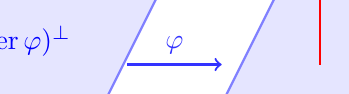
\begin{tikzpicture}[
        plane/.style={fill=blue!10, draw=blue!50, thick}
    ]

    % 坐标系设置
    \coordinate (O) at (0,0,0);

    % 绘制左侧平面 (kerφ)^⊥
    \begin{scope}[transform canvas={xshift=-2.5cm}] % 缩小左侧偏移量
        \draw[plane] (-1.5,-1) -- (1.5,-1) -- (2.5,1) -- (-0.5,1) -- cycle;
        \node[blue] at (0.7,0.3) {$(\ker\varphi)^\perp$};

        % 绘制kerφ箭头(垂直向上)
        \draw[->, thick, red] (0,0) -- (0,2) node[above, left] {$\ker\varphi$};
    \end{scope}

    % 绘制右侧平面 Imφ
    \begin{scope}[transform canvas={xshift=2.0cm}] % 增加右侧偏移量0.5cm
        \draw[plane] (-1.5,-1) -- (1.5,-1) -- (2.5,1) -- (-0.5,1) -- cycle;
        \node[blue] at (0.7,0.3) {$\mathrm{Im}\varphi$};

        % 绘制(Imφ)^⊥箭头
        \draw[->, thick, red] (0,0) -- (0,2) node[above, right] {$(\mathrm{Im}\varphi)^\perp$};
    \end{scope}

    % 绘制水平映射箭头φ(缩短0.5cm)
    \draw[->, thick, blue!80, shorten >=1.25cm, shorten <=1.25cm]
        (-1.7,0) -- node[midway, above] {$\varphi$} (2.0,0); % 调整箭头起点和终点

      \end{tikzpicture}
      \vspace{1cm}
    \caption{$\varphi$映射示意图}\label{fig:kernel_image}
  \end{figure}

  令
  \[
    \xi=\varphi|_{(\ker\varphi)^\perp} :(\ker\varphi)^\perp \to \IM\varphi.
  \]
  则
  \begin{align}
    \ker\xi =& \ker\varphi\cap (\ker\varphi)^\perp=\bm{0},\label{eq:SVD3}\\
    \dim(\ker\varphi)^\perp=& \dim V-\dim\ker\varphi=\dim\IM\varphi.\label{eq:SVD4}
  \end{align}
  由\eqref{eq:SVD3}式可知, $\xi$为单线性映射;
  由\eqref{eq:SVD4}式可知, 线性映射$\xi$的定义域空间和
  值域空间的维数相等,所以$\xi$为满线性映射.从而$\xi$
  一定是线性同构.

  定义
  \begin{align*}
    & \varphi^+=\begin{cases}
      \xi^{-1}(\bm{u}), & \bm{u}\in\IM\varphi,\\
      \bm{0}, & \bm{u}\in(\IM\varphi)^\perp.
    \end{cases}\\
    \Longrightarrow& \varphi^+: U \to V\text{为线性映射}.
  \end{align*}
  考虑$\varphi$的SVD,设
  $V$的一组标准正交基$\{\bm{e}_1,\bm{e}_2,\cdots,\bm{e}_n\}$,
  $U$的一组标准正交基$\{\bm{f}_1,\bm{f}_2,\cdots,\bm{f}_m\}$,
  则
  \begin{align*}
    & \varphi(\bm{e}_i) = \sigma_i\bm{f}_i, 1\leq i \leq r,\\
    & \varphi(\bm{e}_j) = \bm{0}, r+1\leq j \leq n,\\
    & \ker\varphi = L(\bm{e}_{r+1},\cdots,\bm{e}_n),
                  \ker\varphi^\perp = L(\bm{e}_1,\cdots,\bm{e}_r)\\
    & \IM\varphi = L(\bm{f}_1,\cdots,\bm{f}_r),
                  (\IM\varphi)^\perp = L(\bm{f}_{r+1},\cdots,\bm{f}_m).
  \end{align*}
  \[
    \forall 1\leq i \leq r,
    \xi(\bm{e}_i)=\varphi(\bm{e}_i)=\sigma_i\bm{f}_i.
  \]
  因此
  \[
    \varphi^+(\bm{f}_i)=\begin{cases}
      \frac{1}{\sigma_i}\bm{e}_i, & 1\leq i \leq r,\\
      \bm{0}, & r+1\leq i \leq m.
    \end{cases}
  \]
  $\varphi^+$的表示矩阵为
  \[
    \begin{pmatrix}
      \frac{1}{\sigma_1}& & & &\\
                        & \frac{1}{\sigma_2}& & &\\
                        & & \ddots& &\\
                        & & & \frac{1}{\sigma_r}&\\
                        & & & & O
    \end{pmatrix}.
  \]
  由以上两式可验证,定理中的结论(1)(2)(3)都成立.
\end{proof}

\begin{deduction}\label{ded:SVD1}
  设$A\in M_{m\times n}(\mathbb{R})$,则存在唯一的
  $A^+\in M_{n\times m}(\mathbb{R})$满足:

  (1) $AA^+A=A$;

  (2) $A^+AA^+=A^+$;

  (3) $AA^+$和$A^+A$均为是对称阵.

  上述$A^+$称为$A$的Moore-Penrose广义逆.
\end{deduction}

\begin{proof}
  $A$的奇异值分解
  \[
    A=P\begin{pmatrix}
      S&O\\
      O&O
    \end{pmatrix}Q'.
  \]
  则$A^+$的奇异值分解
  \[
    A^+=Q\begin{pmatrix}
      S^{-1}&O\\
      O&O
    \end{pmatrix}P'.
  \]
\end{proof}

\begin{notice}
  \begin{asparaenum}[(1)]
  \item $\varphi, A$可逆时, $\varphi^+=\varphi^{-1}$,
    $A^+=A^{-1}$;
  \item $\varphi=0, A=0$时, $\varphi^+=0, A^+=0$.
  \end{asparaenum}
\end{notice}

\begin{theory}\label{thr:SVD1}
  设$\varphi\in\mathscr{L}(V^n,U^m)$,
  $\varphi^+$是其广义逆,则

  $\varphi^+\varphi$是$V$到$(\ker\varphi)^{\perp}$
  的正交投影算子;

  $\varphi\varphi^+$是$U$到$\IM\varphi$的正交投影算子.
\end{theory}

\begin{proof}
  \begin{align*}
    & \begin{aligned}
      \varphi^+\varphi(\bm{e}_i) & = \varphi^+(\sigma_i\bm{f}_i), 1 \leq i \leq r\\
      & = \frac{1}{\sigma_i}(\sigma_i\bm{e}_i) = \bm{e}_i.
    \end{aligned}\\
    & \varphi^+\varphi(\bm{e}_j) = \bm{0}, r+1\leq j \leq n.
  \end{align*}
  同理可证$\varphi\varphi^+$.
\end{proof}

\begin{theorem}\label{thm:SVD4}
  设$A\in M_{m\times n}(\mathbb{R}), \bm{\beta}\in\mathbb{R}^m,
  \bm{x}\in\mathbb{R}^n$,
  \begin{equation}\tag{*}
    A\bm{x}=\bm{\beta}.
  \end{equation}

  (1)若(*)有解, 则$\bm{z}=A^+\bm{\beta}$是(*)的长度最小的解;

  (2)若(*)无解, 则$\bm{z}=A^+\bm{\beta}$是(*)的最优近似解,即
  \[
    \Vert A\bm{z}-\bm{\beta}\Vert \leq \Vert A\bm{x}-\bm{\beta}\Vert,
    \forall \bm{x}\in\mathbb{R}^n.
  \]
\end{theorem}

\begin{proof}
  (1) 若(*)有解, 则$\bm{\beta}$必在$\IM A$上.
  \[
    \bm{\beta}=A\bm{x}_0, \bm{z}=A^+A\bm{x}_0.
  \]
  则
  \[
    A\bm{z}=A(A^+A\bm{x}_0)=A\bm{x}_0=\bm{\beta}.
  \]
  上式说明$\bm{z}$是(*)的一个解.

    \begin{figure}[hbtp]
    \centering
%    \vspace{1.5cm}
    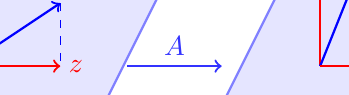
\begin{tikzpicture}[
    plane/.style={fill=blue!10, draw=blue!50, thick},
    projline/.style={dashed, blue, thin} 
]

% 坐标系设置
\coordinate (O) at (0,0,0);

% 左侧平面 (kerA)^⊥
\begin{scope}[transform canvas={xshift=-2.5cm}]
    \draw[plane] (-1.5,-1) -- (1.5,-1) -- (2.5,1) -- (-0.5,1) -- cycle;
    \node[blue] at (0.3,-0.8) {$(\ker A)^\perp$};
    \node[red] at (1.4,0) {$\bm{z}$};
    % kerA箭头
    \draw[->, thick, red] (0,0) -- (0,2) node[above, left] {$\ker A$};
    
    % x0向量及投影
    \draw[->, thick, blue] (0,0) -- (1.2,0.8) node[above left] {$\bm{x}_0$};
    \draw[->, thick, red] (0,0) -- (1.2,0);
    \draw[projline] (1.2,0.8) -- (1.2,0); % 蓝色虚线
\end{scope}

% 右侧平面 ImA
\begin{scope}[transform canvas={xshift=2.0cm}]
    \draw[plane] (-1.5,-1) -- (1.5,-1) -- (2.5,1) -- (-0.5,1) -- cycle;
    \node[blue] at (0.3,-0.8) {$\mathrm{Im}A$};
    \node[red] at (1.2,0) {$AA^+\bm{\beta}$};
    % (ImA)^⊥箭头
    \draw[->, thick, red] (0,0) -- (0,2) node[above, left] {$(\mathrm{Im}A)^\perp$};
    
    % beta向量及投影
    \draw[->, thick, blue] (0,0) -- (0.6,1.5) node[above right] {$\bm{\beta}$};
    \draw[->, thick, red] (0,0) -- (0.6,0);
    \draw[projline] (0.6,1.5) -- (0.6,0); % 蓝色虚线
\end{scope}

% 映射箭头A
\draw[->, thick, blue!80, shorten >=1.25cm, shorten <=1.25cm]
    (-1.7,0) -- node[midway, above] {$A$} (2.0,0);

  \end{tikzpicture}
  \vspace{1cm}
    \caption{矩阵$A$表示的线性映射示意图}
    \label{fig:SVD2}
  \end{figure}
  设$\bm{x}_0$是(*)的一个解, 如图\ref{fig:SVD2}所示:
  由于$\ker A$在矩阵$A$的作用下等于0,因此$\bm{x}_0$与$\ker A$中
  任一元素的和都是(*)的解.对$\bm{x}_0$做正交直和分解,这是
  长度最小的解.由引理\ref{thr:SVD1}(1)可知, $\bm{x}_0$的正交直和分解
  即$A^+A\bm{x}_0=\bm{z}$.

  (2) 若(*)无解, 则$\bm{\beta}$必不在$\IM A$上.
  \[
    A\bm{z} = A(A^+\bm{\beta})\perp (\IM A)^\perp.
  \]
  \[
    A\bm{x}-\bm{\beta}=A(\bm{x}-\bm{z})+A{\bm{z}}-\bm{\beta},
  \]
  由于$A(\bm{x}-\bm{z})\in\IM A, A\bm{z}-\bm{\beta}\in (\IM A)^\perp$,
  根据勾股定理,有
  \[
    \Vert A\bm{x}-\bm{\beta}\Vert \geq \Vert A\bm{z}-\bm{\beta}\Vert.
  \]
\end{proof}

\begin{remark}
  在经济和金融等生产实际中,常常可以根据
  实际数据得到大量的矛盾方程组:
  \[
  A^{m\times n}\bm{x}^{n\times 1}=\bm{\beta}^{m\times 1},
\]
由于实际可得的数量充分多,因此$m\gg 0$,即矩阵的行数可以特别多,
方程数量可以很多,从而只能保证列满秩$\rank(A)=n$.
根据定理\ref{thm:SVD4},可以得到最优解(最佳逼近解)
  \[
    \bm{x}=A^+\bm{\beta} \xlongequal{A^+=(A'A)^{-1}A'}
    (A'A)^{-1}A'\bm{\beta}.
\]
即9.4节中的最小二乘法.
\end{remark}
%%% Local Variables:
%%% mode: latex
%%% TeX-master: "../main"
%%% End:
